%!TEX root=../Thesis_Zepeng.tex
\chapter{Handling general loadings}\label{chp:5}
\minitoc

\section{Multiscale energy dissipation approach}
\label{sec:5.1}
Fatigue failure is a damage accumulation process in which material property deteriorates continuously under fatigue loading and the damage depends on the size of stress and strain. With the accumulation of fatigue damage, some accidents occur for these components. Thus, it is important to formulate an accurate method to evaluate the fatigue damage accumulation and effectively predict the fatigue life of these components even when subjected to complex loadings.

The problem is then to define criteria able to predict this endurance limit. The micro-macro approach applied to the field of endurance was born with the work of \cite{van1973khmu}, and since it has been used many times, including by \cite{papadopoulos2001long} to take better account of loading path effects. For simplicity and to avoid too costly identification procedures of fatigue data, criteria are often expressed using two parameters. The first relates generally to a shear stress $\tau$ (on a plane or on average over an elementary volume) while the second $\sigma$ reflects the normal stress effects (mean and amplitude) often through the hydrostatic stress are the most numerous (\cite{crossland1956effect}, \cite{sines1959behavior}, \cite{FFE:FFE452}, \cite{thu2008effet}).  The normal stress acting on the material plane is sometimes defined from a critical plane(\cite{findley1959}), or through integration at every plane of an elementary volume(\cite{liu1993berechnung}).  In particular, a probabilistic approach based on this type of integration is proposed in \cite{thu2008effet} .

Other authors use energy based approaches. \cite{ellyin1974criterion} is one of the first to propose a fatigue criterion based on cyclic shear deformation energy. This approach was taken up and complemented by \cite{lefebvre1981cognitive} and \cite{ellyin1991phase} for the case of multiaxial loadings. In France, this approach is reflected in the work of \cite{Froustey1992} and then in \cite{palin1996fatigue} and \cite{banvillet2001prevision}. In recent years, a new class of criteria coupling mesoplasticity and damage has also emerged. In \cite{lemaitre1999two}, for example, the author use the approach introduced by \cite{lemaitre1985mecanique} based on the thermodynamics of irreversible processes and the mechanics of continuous media.   Models based on plasticity-damage coupling were also proposed in \cite{flaceliere2004contribution},\cite{monchiet2006contributions}. In the case of fatigue, we usually employ in this damage framework the concept of the loading cycle instead of time to evaluate the evolution of damage and to measure the fatigue lifetime. The equations then depend on the load through globally defined quantities over a cycle, such as amplitude, maximum value, mean value. The growth equation of fatigue damage is therefore taken in the form as described in Chapter \ref{chp:4}:
$$\delta D=f(D)\delta N$$
$$\delta N=f_n\delta t$$
where $\delta t$ is a time sampling of the history in a given number of time intervals $\delta t_1,\delta t_2 ... \delta t_i, ...$ and $f_n$ is the mean frequency of those cycles during the considered time step.

The problem in these approaches is then to take into account the presence of complex variations of the stress tensor. Heuristic formulations with different multiaxial fatigue criteria have been proposed, but most of them still requires the notion of load cycles. The objective of the present chapter is to contribute to the development of life models that take into account such complex variations while avoiding the notion of load cycle. Our fundamental thought is to assume within a micro-macro approach that the local dissipated energy at small scale contributes to the damage which governs fatigue at failure. We follow the Dang Van paradigm. The structure is elastic  at the macroscopic scale. At each material point, there is a stochastic distribution of weak points which will undergo strong plastic yielding, which contributes to energy dissipation and cause damage, without affecting the overall macroscopic stress.

Our model considers a plastic behavior at the mesoscopic scales  with a dependence of the yield function not only on the deviatoric part of the stress but also on the hydrostatic part. A kinematic hardening under the assumption of associative plasticity is also introduced.

Instead of using the number of cycles, we will use in addition as in \cite{lemaitre1999two} the concept of nonlinear damage accumulation during the loading history. To approach real life loading history more accurately, non-linear damage accumulation laws are also considered in our model to take into account the sequencing effect. Fatigue will then be determined from the energy plastically dissipated at all scales during plastic shakedown cycles and from a phenomenological fatigue law linking damage evolution and accumulated mesoscopic plastic dissipation.

The chapter is organized as follows. From section \ref{sec:5.1} to \ref{sec:5.3}, we present the existing methods and background of our strategy.  In section \ref{sec:5.4} we propose the notion of weakening scales and multiscale yield function and describe the plastic dissipation resulting from this notion. And in section \ref{sec:5.5}, based on microscopic plasticity we construct the energy dissipation formula. Section \ref{sec:5.6} gives the proposed nonlinear damage accumulation law and summarizes the full model that we propose. Then we combine the energy dissipation law and nonlinear damage accumulation law with its numerical implementation presented in section \ref{sec:5.7}, while section \ref{sec:5.8} is devoted to various validations on typical load histories classically treated in the literature. Parameter identification strategy is presented in section \ref{sec:5.9}.



\section{Kinematic Hardening Models}
\subsection{Linear Kinematic Hardening}
A hardening rule is needed in microplasticiy to
describe the behavior of the
material once it is plastically
deformed or yielded. One possible hardening rule is the
isotropic rule, which assumes
that strain hardening corresponds
to an enlargement of the yield
surface (i.e. an increase in  yield stress )
without change of shape or
position in the stress space. Another is the kinematic rule,
which assumes that strain
hardening shifts the yield surface
without changing its size or shape.
\begin{figure}[h!]
	\centering
	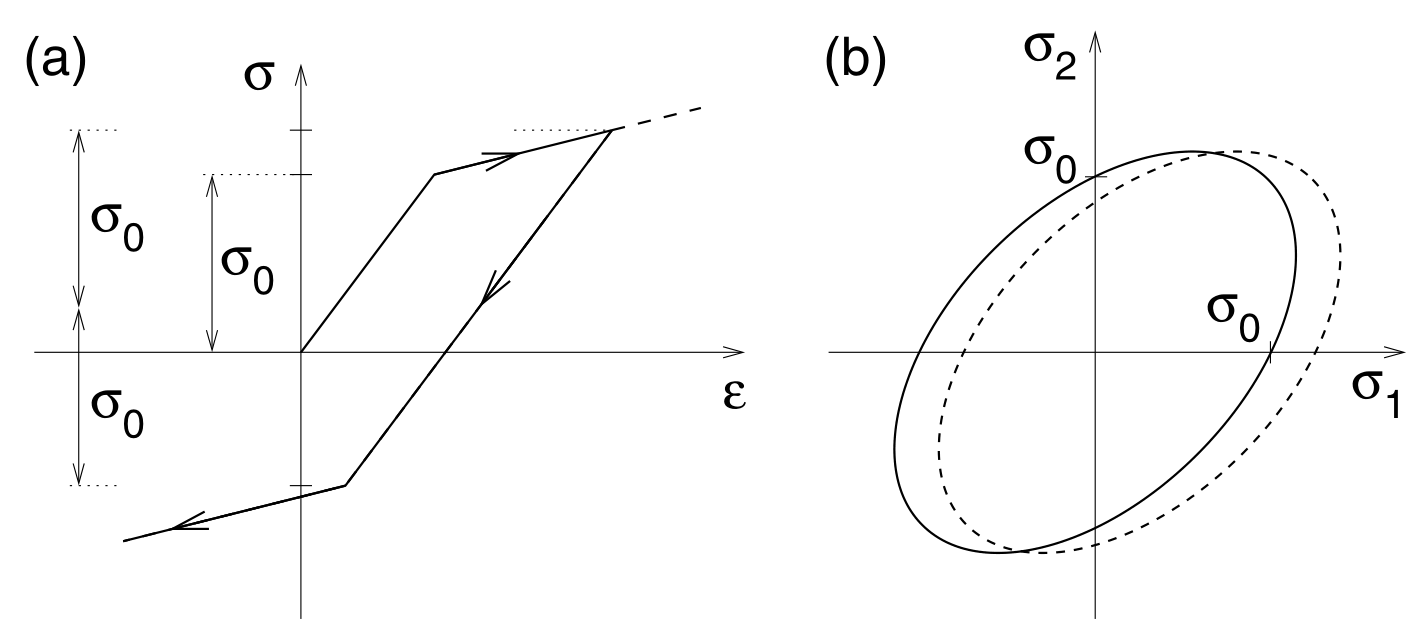
\includegraphics[width=0.8\textwidth]{figures//kinhard.png} 
	\caption{Kinematic hardening: a) uniaxial stress-strain diagram, b) evolution of the
		yield surface in the biaxial stress plane}
	\label{kinhard}
\end{figure}
Kinematic hardening rules are necessary,especially for the case of unloading and cyclic loading.In Kinematic Hardening the current loading surface is assumed not to expand but to move as a rigid body
within the stress space (\figref{kinhard}(b)). The use
of kinematic hardening is, for example, necessary to model the so-called Bauschinger
effect (Bauschinger, 1881). This effect is often observed in metals subjected to cyclic
loading. Even if the magnitudes of the yield stress in tension and in compression
are initially the same, this is no longer the case when the material is preloaded into
the plastic range and then unloaded. For example, after previous yielding in tension,
yielding in compression may start at a stress level lower than the initial yield stress
(\figref{kinhard}(a)).

Kinematic hardening leads to a translation of the loading surface, i.e. to a shift of
the origin of the initial yield surface. If the initial yield surface is described by a yield
function of the form
$$f(\sigma) = F(\sigma) -\sigma_0 $$
the shifted surface is obviously described by
$$f(\sigma,\sigma_b ) = F(\sigma-\sigma_b ) -\sigma_0$$
where $\sigma_b$ is the so-called backstress that represents the center of the shifted elastic
domain and plays the role of a tensorial hardening variable. Now we need a kinematic
hardening law that governs the evolution of the back stress. \cite{melan1938plastizitat} proposed
a law of the form
\begin{equation}
\dot{\sigma}_b =\overline{H}_K \dot{\varepsilon}_p
\label{lineark}
\end{equation}
where $ \dot{\varepsilon}_p$ is the rate of effective plastic strain. According to which the rate of the back stress is proportional to the plastic strain rate. It is a macroscopic variable representing the
dislocation sub-structure resistance to deformation. 
The proportionality factor $\overline{H}_K$ is directly related to the plastic modulus and is derived from a simple
monotonic uniaxial curve.The linear hardening law Eq.\eqref{lineark} is often credited to Prager (1955, 1956); we will call it the Melan–Prager hardening rule. 
\subsection{Non-linear Kinematic Hardening}
%\begin{figure}[h!]
%		\includegraphics[width=\textwidth]{figures//kinehardening.gif} 
%		\caption{Dissipated energy in one cycle and number of cycles %to failure when $\beta=-1$}
%		\label{kinehardening}
%\end{figure}
To describe cyclic plasticity, one of the famous model is the non-linear kinematic hardening model formulated by Armstrong and Frederick. It is based on a physical mechanism of strain hardening and dynamic recovery and is capable of simulating the
multiaxial Bauschinger effect (movement of the yield surface in the stress space). Therefore, the model has been examined and implemented in commercial software and finite element analysis.

The Armstrong-Frederick model (AF) is a modification of the Melan–Prager linear kinematic hardening model. The only modification of this simple model is the "recal" term which changes the evolution law for the symmetric backstress tensor $\sigma_b$ from a classical linear kinematic hardening law (Melan–Prager) to a nonlinear kinematic hardening law. The term is proportional to the current back stress multiplied by the norm of the plastic strain rate. According to the Armstrong-Frederick rule, the evolution of the
back stress is governed by the differential equation:

\begin{equation}
\dot{\bm{\sigma}}_b=\underbrace{\overline{H}_K \dot{\varepsilon}_p}_{lin. kin. hardening} -\underbrace{\gamma\dot{p}\bm{\sigma}_b}_{recall - term, nonlinear hardening}
\label{nonlineark}
\end{equation}
where
$\dot{p}$ is the accumulated plastic strain rate given as $\sqrt{\dfrac{2}{3}}||\dot{\varepsilon}_p||$ . The constants
$\overline{H}_K$
and
$\gamma$
are determined from uniaxial tests.
At the onset of yielding, the
back stress is still zero and Eq.\eqref{nonlineark} gives the same response as the linear hardening
law Eq.\eqref{lineark}. As the back stress develops, the additional term becomes activated and
slows down the rate at which the back stress grows (i.e. reduces the tangent plastic
modulus).

\section{Mean stress effect in local model}
\label{sec:5.3}
Positive mean stress clearly reduces the fatigue life of the material. In design evaluation of multiaxial fatigue with mean stress, a simplified, conservative relation between mean stress and equivalent alternating stress is necessary. We can improve the model by modifying the yield function $\sigma_y$ and the localization tensor in order to take mean stress effect into account.

\vspace{6pt}
\textbf{Christensen approach}
\vspace{6pt}

The yield function that was given by \cite{christensen2000yield} integrates measures of damage, as well as intrinsic yield strength and concept of transitions. The derived yield function formalism resulted in the form as:

\begin{equation}
\frac{\alpha K}{\sqrt{3}}\sigma_{kk}+\frac{(1+\alpha)^2}{2}s_{ij}s_{ij}\leqslant\frac{K^2}{(1+\alpha)}.
\label{eq:yieldfunc}
\end{equation}
Here $\alpha$ changes the shape of the yield function, thus it is called the shape parameter. 
$$\alpha=\frac{\left| \sigma_{11}^C\right| }{\sigma_{11}^T}-1.$$
The new parameter $K$ is called the ideal or intrinsic strength which uniformly expands or contrasts the yield function, thus is is called the scale parameter:
$$K=\frac{(\sigma_{11}^C)^2}{\sqrt{3}\sigma_{11}^T}.$$
The intrinsic strength would occur if there were no damage or microstructure disturbance. 
$\sigma_{11}^C$ and $\sigma_{11}^T$ are respectively compressive and tensile yield stress in uniaxial states where $\left| \sigma_{11}^C\right| \geqslant\sigma_{11}^T$(for ductile materials, $\frac{1}{2}\leqslant\dfrac{\left| \sigma_{11}^C\right| }{\sigma_{11}^T}\leqslant 1$). The yield stress in uniaxial and shear states are given by:

\begin{equation}
\begin{split}
&\sigma_{11}^C=\frac{-\sqrt{3}K}{(1+\alpha)}\\
&\sigma_{12}^Y=\frac{K}{(1+\alpha)^{3/2}} \\
&\sigma_{11}^T=\frac{\sqrt{3}K}{(1+\alpha)^2}.\\
\end{split}
\label{eq:uniyields}
\end{equation}

At $\alpha=0$, relations Eq.\eqref{eq:yieldfunc} and Eq.\eqref{eq:uniyields} show the behavior to be that of purely Mises type. This is taken to be the ideal condition where the intrinsic strength $K$ solely determines the yield strength. As the shape parameter increases beyond the value $\alpha=1$, the yield function behaves in accordance with  a state of increasing crack density or any other physical weakening. The term fracture, as used here for behavior at or near $\alpha=1$, actually corresponds to fracture mechanics for non-interacting cracks. Beyond this range near $\alpha=1$ or $\alpha\to\infty$ has simply been called yield or failure. Parameter $\alpha$ could be easily viewed as a damage measure or microstructure parameter since it represents microstructure changes on any scale that causes deviation from the ideal state. 

It is concluded a decrease in mean stress $\sigma_{kk}$ reduces the effective value of $\alpha$. That is, moving the behavior toward ductile case. Alternatively, increasing the mean stress moves $\alpha$ toward larger values, which is taken to be that of brittle behavior.

The fully expanded form of the yield function Eq.\eqref{eq:yieldfunc} is:
\begin{equation}
\begin{split}
&\frac{\alpha K}{\sqrt{3}}(\sigma_{11}+\sigma_{22}+\sigma_{33})\\
+&(1+\alpha)^2\left[\frac{(\sigma_{11}-\sigma_{22})^2+(\sigma_{22}-\sigma_{33})^2+(\sigma_{33}-\sigma_{11})^2}{6}
+(\sigma_{12}^2+\sigma_{23}^2+\sigma_{31}^2) \right]\\
\leqslant&\frac{K^2}{(1+\alpha)}.\\
\end{split}
\end{equation}

The most compact form of Eq.\eqref{eq:yieldfunc} is:
\begin{equation}
\frac{1}{2}s_{ij}s_{ij}\leqslant\eta K^2,
\end{equation}
where $\eta$ is a nondimensional scaling factor on $K^2$, determined by mean normal stress.
$$\eta=\frac{1-\dfrac{\alpha(1+\alpha)}{\sqrt{3}K}\sigma_{kk}}{(1+\alpha)^3}<1$$


The mean stress $\sigma_{kk}$ has a positive relationship with the shape parameter $\alpha$. We suppose the material endures transition from ductile to brittle when $\alpha$ reaches 1. That means $\alpha$ has a very similar physical meaning with the damage parameter $D$.

\vspace{6pt}
\textbf{The Gerber parabola}
\vspace{6pt}

Several models are available addressing the influence of tensile mean stress on fatigue life. Among these are the Gerber (Germany, 1874), Goodman (England, 1899), and Soderberg (USA, 1930) models.  The modified Goodman criterion is often used as a design criterion because it is more conservative than the Gerber criterion. The use of the Gerber criterion in the determination of member size is generally more computationally  intensive and so rather unattractive for many designers.

The effect of mean stress on the fatigue strength is commonly presented in Haigh diagrams as shown in \figref{haigh}, where $S_a / S_f$ is plotted against $S_m / S_u$ at fatigue limit. $S_a$ is the fatigue strength at a given life under fully reversed ($S_m = 0$,$R = -1$) conditions. $S_u$ is the ultimate tensile strength. $S_f$ is the reversed fatigue strength in absence of mean stress. The data points thus represent combinations of $S_a$ and $S_m$ giving that life. The results were obtained for small unnotched specimens, tested at various tensile mean stresses. The straight lines are the modified Goodman and the Soderberg lines, and the curved line is the Gerber parabola. These are empirical relationships that are represented by the following equations:

\vspace{6pt}
Modified Goodman: $S_a/S_f + S_m/S_u = 1$

\vspace{6pt}
Gerber: $S_a/ S_f + (S_m/ S_u)^2 = 1$

\vspace{6pt}
Soderberg: $S_a/S_f+S_m/S_y=1$

\begin{figure}[h!]
	\centering
	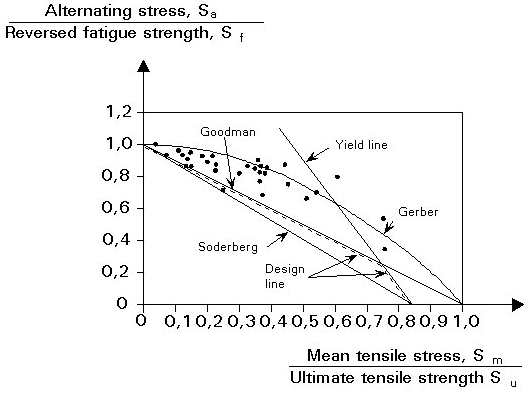
\includegraphics[width=0.8\textwidth]{figures//Gerber.png} 
	\caption{Haigh diagram showing test data points for the effect of mean stress, and the Gerber, modified Goodman and Soderberg relations.}
	\label{haigh}
\end{figure}

In the following section, we introduce the sale dependent mean stress effect in our model.

\section{Weakening scales and yield function}
\label{sec:5.4}
\subsection{The concept of weakening scales} 

We follow the Dang Van paradigm. The structure is elastic at the macroscopic scale. At each material points, there is a stochastic distribution of weak points which will undergo strong plastic yielding, without contributing to the overall macroscopic stress. From a microscopic point of view, there is a distribution of weakening scales, namely $s\in[1,\infty)$. In order to introduce our concept, lest us imagine that we can measure the macroscopic stress intensity at present time by a given value $S_{a}$. Let $\sigma_y$ be the yield limit before weakening. Then we imagine that for a given scale $s$:

\vspace{6pt}
\noindent
$\bullet$ either $1\leqslant s\leqslant \sigma_y/S_{a}$, then $S_{a}\leqslant \sigma_y/s$, the material stays in the elastic regime and there is no energy dissipation at this scale.

\vspace{6pt}
\noindent
$\bullet$ or $\sigma_y/S_{a}\leqslant s\leqslant \infty$, then $S_{a}\geqslant \sigma_y/s$, the material is in plastic regime at this scale, which evolves through kinematic hardening, say from zero initial plastic strain $\uuline{\varepsilon}_p(s)$ and zero initial backstress $\uuline{b}(s)$ at initial time $t_0$. There is then dissipated energy at scale $s$ contributing to the fatigue limit.


\vspace{6pt}

\subsection{Distribution of weakening scales}

We assume the weakening scales have a  probability distribution function following a power law:
\begin{equation}
P(s) = Hs^{-\beta}=(\beta-1)s^{-\beta},
\label{eq.ps}
\end{equation}

where $\beta$ is a material constant. 
The choice of a power law comes with two reasons: on one hand, this type of distribution corresponds to a scale invariant process, on the other hand it leads in cyclic loading to a prediction of a number of cycles to life limit as a power law function of the stress intensity. More general laws can also be proposed, without changing the spirit of the model.

%The integrated probability ranging from macroscopic to microscopic stress  is unity. From this we can conclude:
%$$\int_{1}^{\infty}P(s)ds=\left[ \frac{Hs^{1-\beta}}{1-\beta}\right] _{1}^{\infty}=0-\frac{H}{1-\beta}=1.$$
%Then we know $H=\beta-1$, so the distribution is given by:
%$$P(s) = Hs^{-\beta}=(\beta-1)s^{-\beta}$$
The probability of weakening scales is shown in \figref{ps1} and \figref{ps2}. We can see that smaller $\beta$ leads to larger probability of weakening for large $s$.
\begin{figure}[!h]
\centering
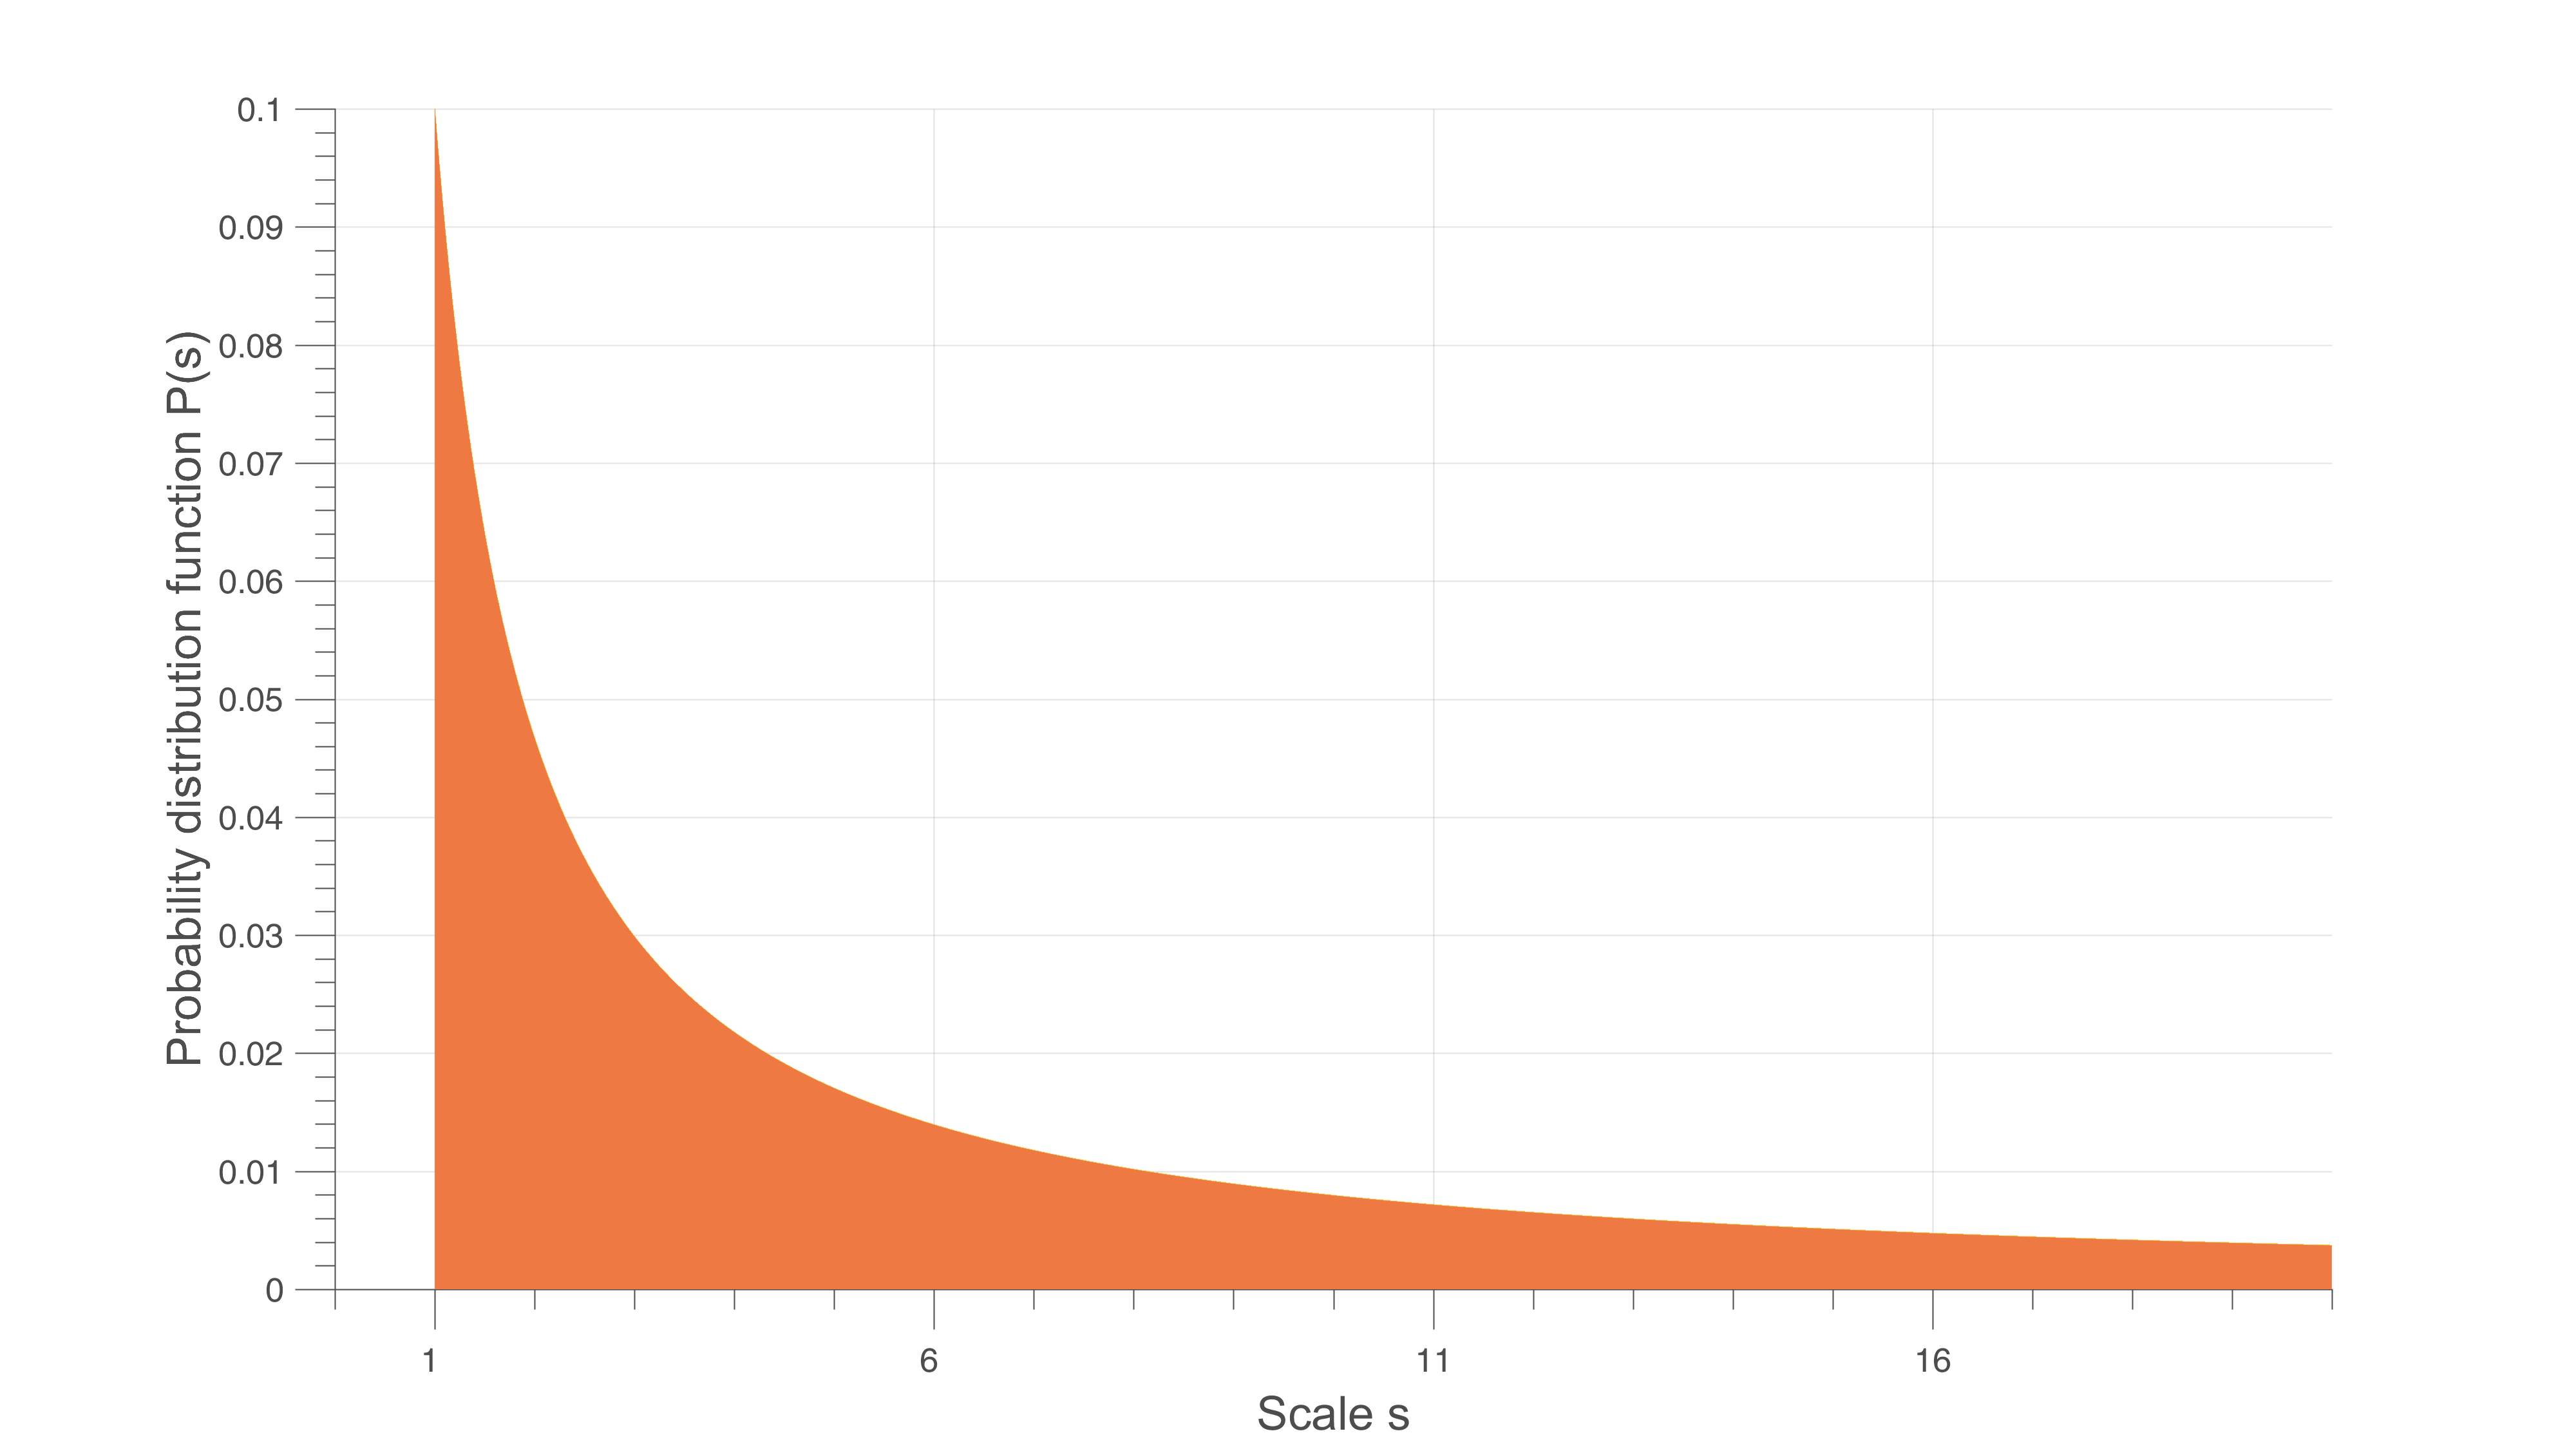
\includegraphics[width=0.9\textwidth]{figures//ps1.png} 
\caption{Weakening scales $s$ probability distribution curve when $\beta=1.5$ }
\label{ps1}
\end{figure}
\begin{figure}[!h]
\centering
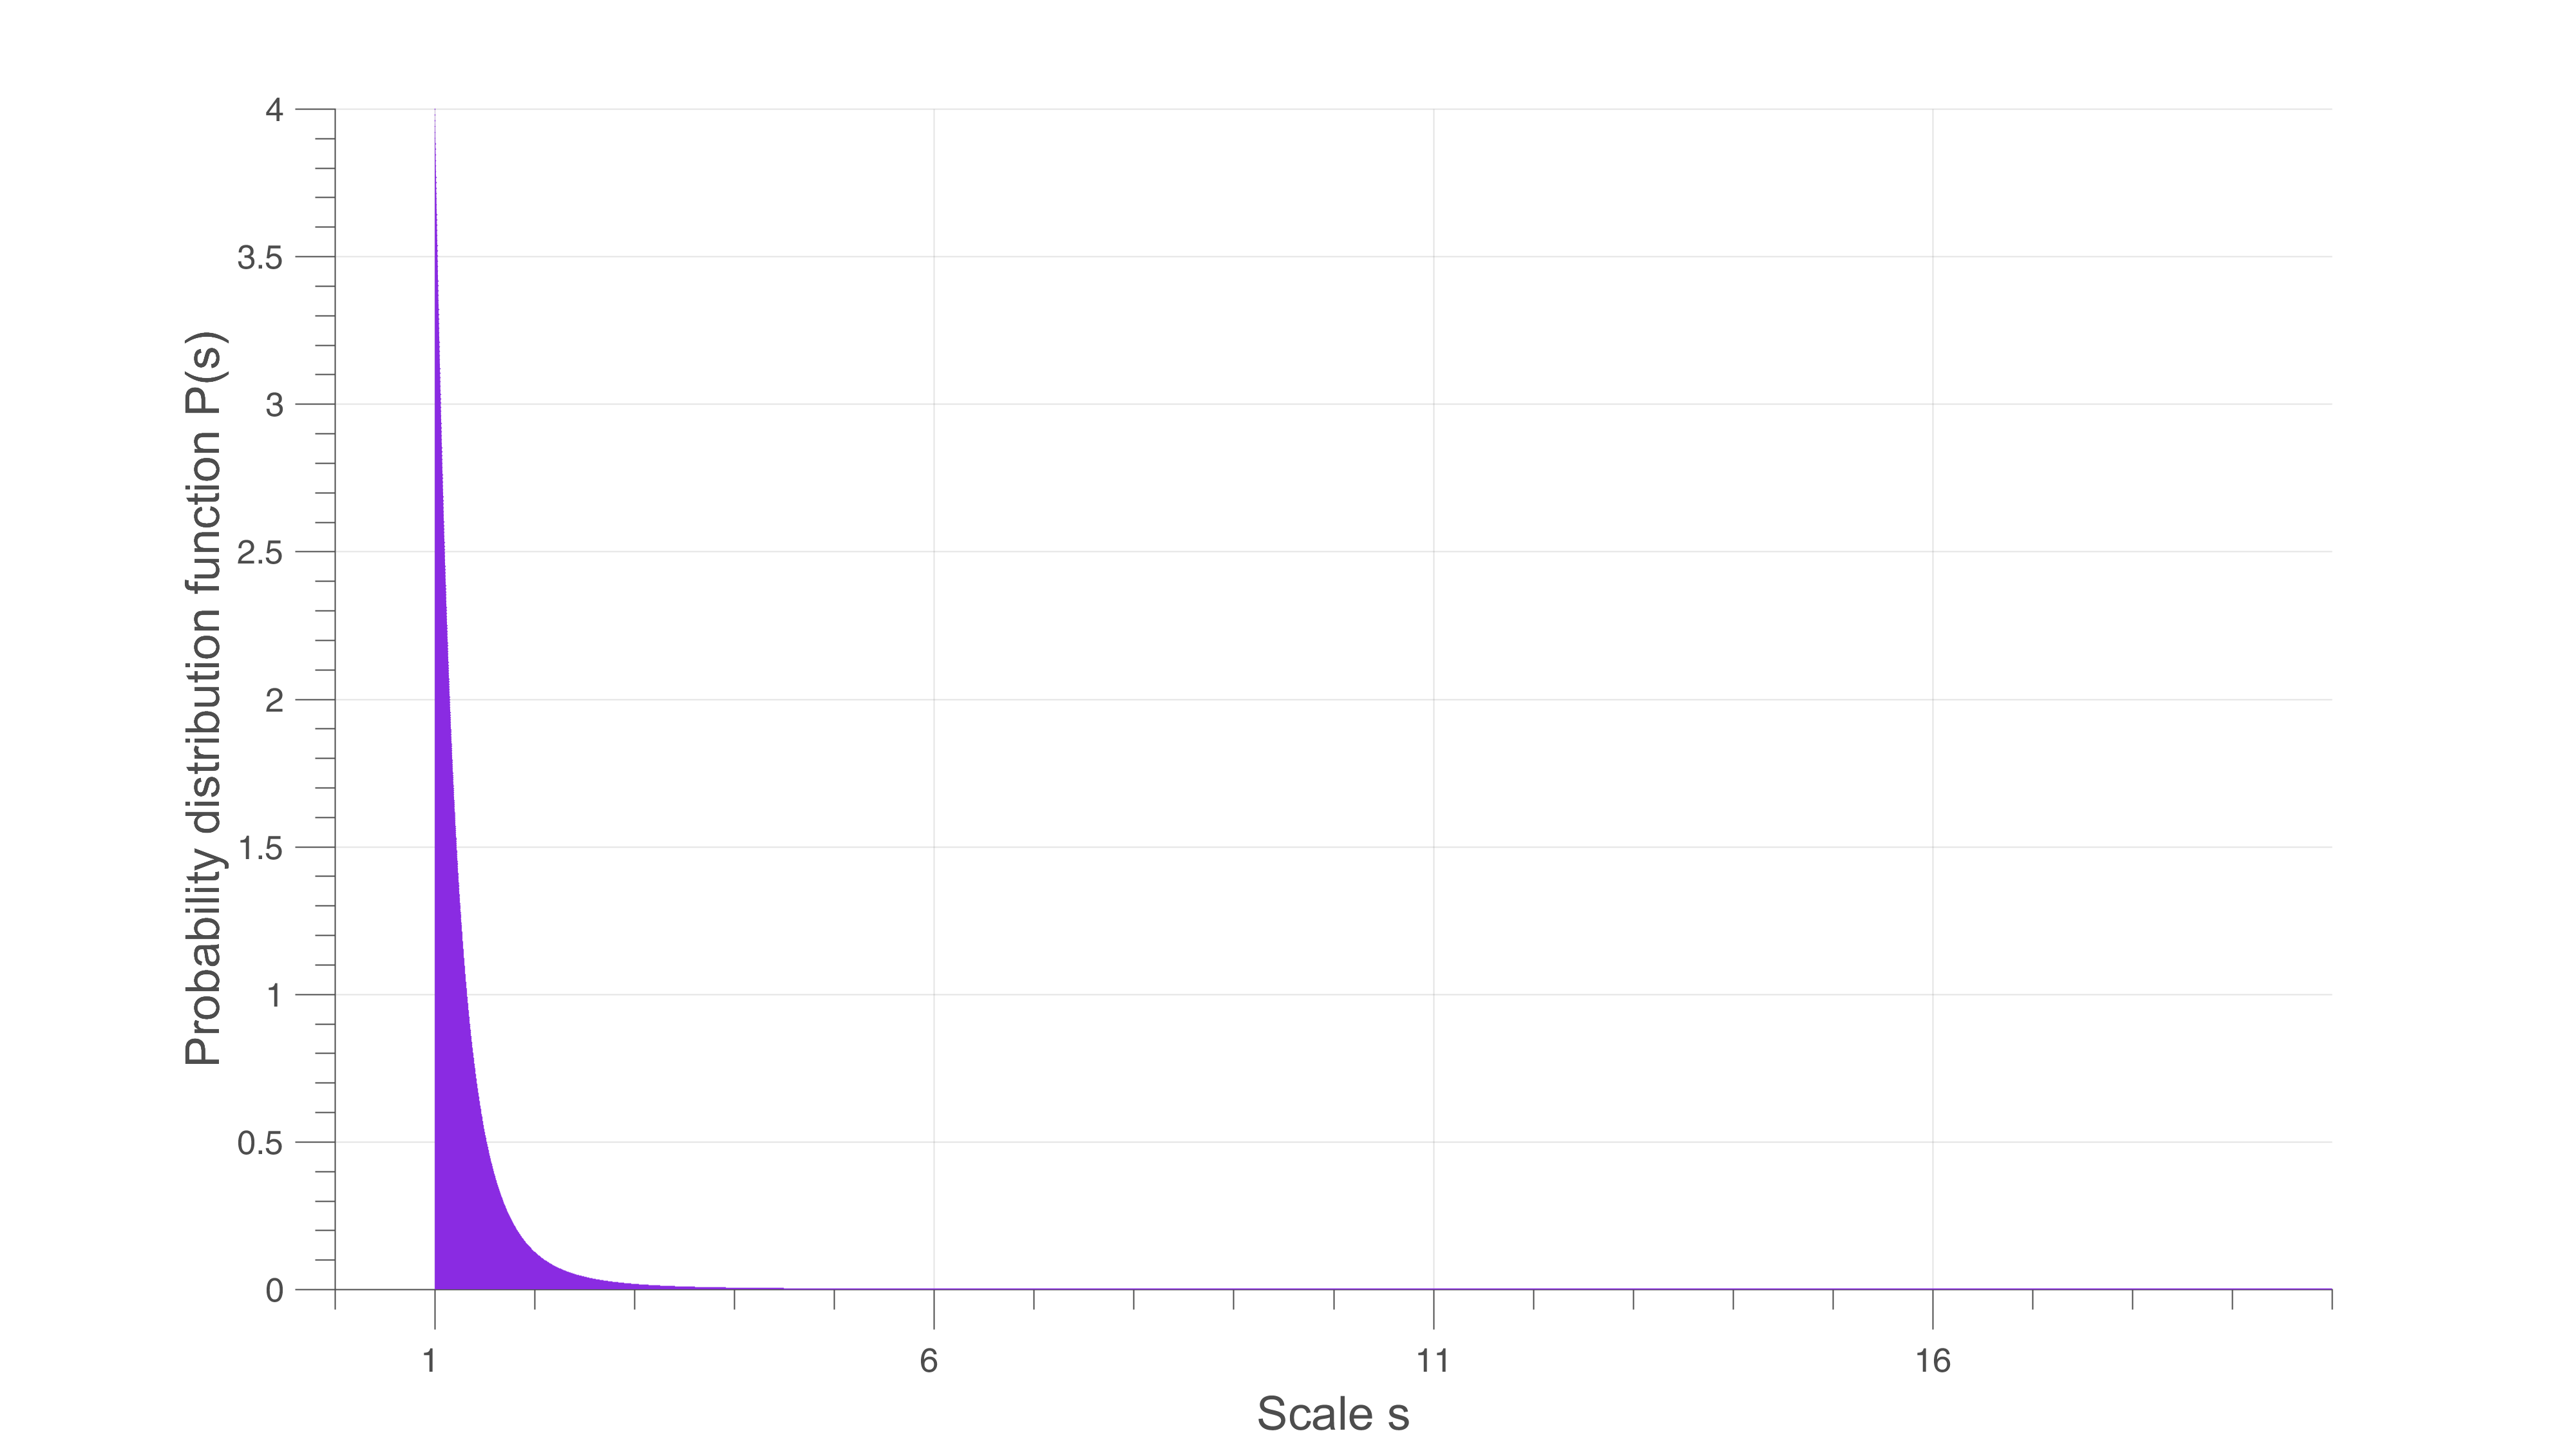
\includegraphics[width=0.9\textwidth]{figures//ps2.png} 
\caption{Weakening scales $s$ probability distribution curve when $\beta=5$ }
\label{ps2}
\end{figure}

\newpage
\subsection{Yield function with mean stress effect}
\label{sec:5.4.3}
Positive mean stress clearly reduces the fatigue life of the material. In design evaluation of multiaxial fatigue with mean stress, a simplified, conservative relation between mean stress and equivalent alternating stress is necessary. We can improve the model to come by modifying the yield function $\sigma_y$ and the localization tensor.

\vspace{6pt}
\textbf{Present choice}
\vspace{6pt}

In the model to come, our idea is to consider as in \cite{Maitournam2011232} that the yield limit $\sigma_y$ can be reduced in presence of positive mean stress. The mesoscopic yield function can therefore be written as:
\begin{equation}
f\left(s\right)=||\uline{\uline{S}}(s)-\uline{\uline{b}}(s)||+\left( \lambda \Sigma_H-\sigma_y\right) /s\leqslant 0
\label{eq.yieldfun}
\end{equation}
with $\uline{\uline{S}}$ denoting the deviatoric part of the stress tensor at microscale, and $\uline{\uline{b}}(s)$ the corresponding backstress at the same scale. The material remain in elastic regime when $f<0$ and in plastic regime when $f=0$. The parameter $\lambda$ can itself be a function of $\Sigma_H$ with a different value in traction($\lambda_+$) than in compression($\lambda_-$).


\subsection{Local plastic model}
We can now describe the mesoscopic stress state.  The model considers a plastic 
behavior at the mesoscopic scale. The mesoscopic stress evolution equations are thus:

\begin{equation}
\dot{\uline{\uline{S}}}(s,M,t)=dev\dot{\uline{\uline{\Sigma}}}(M,t)-\dfrac{E}{1+\nu}\dot{\uline{\uline{\varepsilon}}}^p(s,M,t), 
\label{eq.mesostress}
\end{equation}
which defines a Taylor-Lin scale transition model with unit localization tensor (\cite{Bosia201239}). The mesoscopic deviatoric strain rate tensor is thus equal to the macroscopic strain rate tensor $dev\dot{\uline{\uline{\Sigma}}}=\dfrac{1+\nu}{E}dev\dot{\uline{\uline{\varepsilon}}}$ with $dev\uline{\uline{\Sigma}}$ the deviatoric part of the macroscopic stress tensor. It is complemented by
\begin{equation}
\dot{\uline{\uline{b}}}(s,M,t)=\dfrac{kE}{E-k} \dot{\uline{\uline{\varepsilon}}}^p(s,M,t), 
\label{eq.backstress}
\end{equation}
which is our kinematic hardening model, and by
\begin{equation}
\dot{\uline{\uline{\varepsilon}}}^p(s,M,t)=C\dfrac{\partial f(s,M,t)}{\partial \uline{\uline{S}}}, 
\label{eq.plasticflow}
\end{equation}
which is the associated plastic flow rule assuming $C=0$ when $f<0$ and  $C\geqslant0$ when $f=0$.

Here E denotes the Young's modulus and k the hardening parameter. The local dissipated energy rate per unit volume at weakening scales $s$  is given by the local entropy dissipation:
\begin{equation}
\dot{w}(s,M,t)=(\uuline{S}-\uuline{b})(s,M,t):\uuline{\dot{\varepsilon}}^p(s,M,t).
\label{dissipated}
\end{equation}

\section{Construction of an energy based fatigue approach}
\label{sec:5.5}
In a preliminary step, we will consider a simple macroscopic loading history $\uuline{\Sigma}(M, t)$ which is uniaxial
 along direction $\uline{\uline{s}}_1$, with $\uline{\uline{s}}_1$ a given stress tensor of unit norm. In traction there is 
 $$\uline{\uline{s}}_1=\sqrt{\dfrac{3}{2}}	\left(
 \begin{array}{ccc}
2/3 & 0 & 0\\
 0 & -1/3 & 0\\ 
 0 & 0 & -1/3\\
 \end{array}\right) . $$
  Time periodic of deviatoric amplitude $S_{a}$, constant mean stress $\Sigma_{H}$ and a Von Mises flow rule are taken into account to see if we get a prediction of local failure for a number of cycles $N_F$ varying as $S_{a}^{-\gamma}.$

In uniaxial cyclic loading, there will be 3 kinds of loading patterns, as is shown in \figref{backstress}:

\vspace{6pt}
\begin{enumerate}

\item	Elastic regime, in phase 2 and 4,where we have no plastic flow $\dot{\uline{\uline{\varepsilon}}}^p(s,M,t)=\dot{\uline{\uline{b}}}=0$ ,  and where the stress is below the yield limit $|\uline{\uline{S}}-\uline{\uline{b}}|< \left( \sigma_y-\lambda \Sigma_H\right)/s$, and where we have therefore $\dot{\uline{\uline{S}}}=dev\dot{\uline{\uline{\Sigma}}}$. 
\vspace{6pt}

\item Plastic regime according to plastic flow rule, with increasing plastic deformation, in phase 5 and 1, where	$\dot{\uline{\uline{\varepsilon}}}^p(s,M,t)=\xi\dfrac{\uline{\uline{S}}(s)-\uline{\uline{b}}(s)}{||\uline{\uline{S}}(s)-\uline{\uline{b}}(s)||}> 0$ with  $\xi= \left| dev\dot{\uline{\uline{\Sigma}}}\right| \left(\dfrac{kE}{E-k}+\dfrac{E}{1+\nu} \right) ^{-1}$(detailed in annex) ,  $\uline{\uline{S}}-\uline{\uline{b}}=\uline{\uline{s}}_1 \left(\sigma_y-\lambda \Sigma_H\right)/s$ and $\dot{\uline{\uline{S}}}-\dot{\uline{\uline{b}}}=0.$ 
\vspace{6pt}

\item Plastic regime in the other direction, in phase 3, where we now have	$\dot{\uline{\uline{\varepsilon}}}^p(s,M,t)<0$,  then $\uline{\uline{S}}-\uline{\uline{b}}=-\uline{\uline{s}}_1 \left(\sigma_y-\lambda \Sigma_H\right)/s$ and $\dot{\uline{\uline{S}}}-\dot{\uline{\uline{b}}}=0$.

\end{enumerate}	

\begin{figure}[!h]
\centering
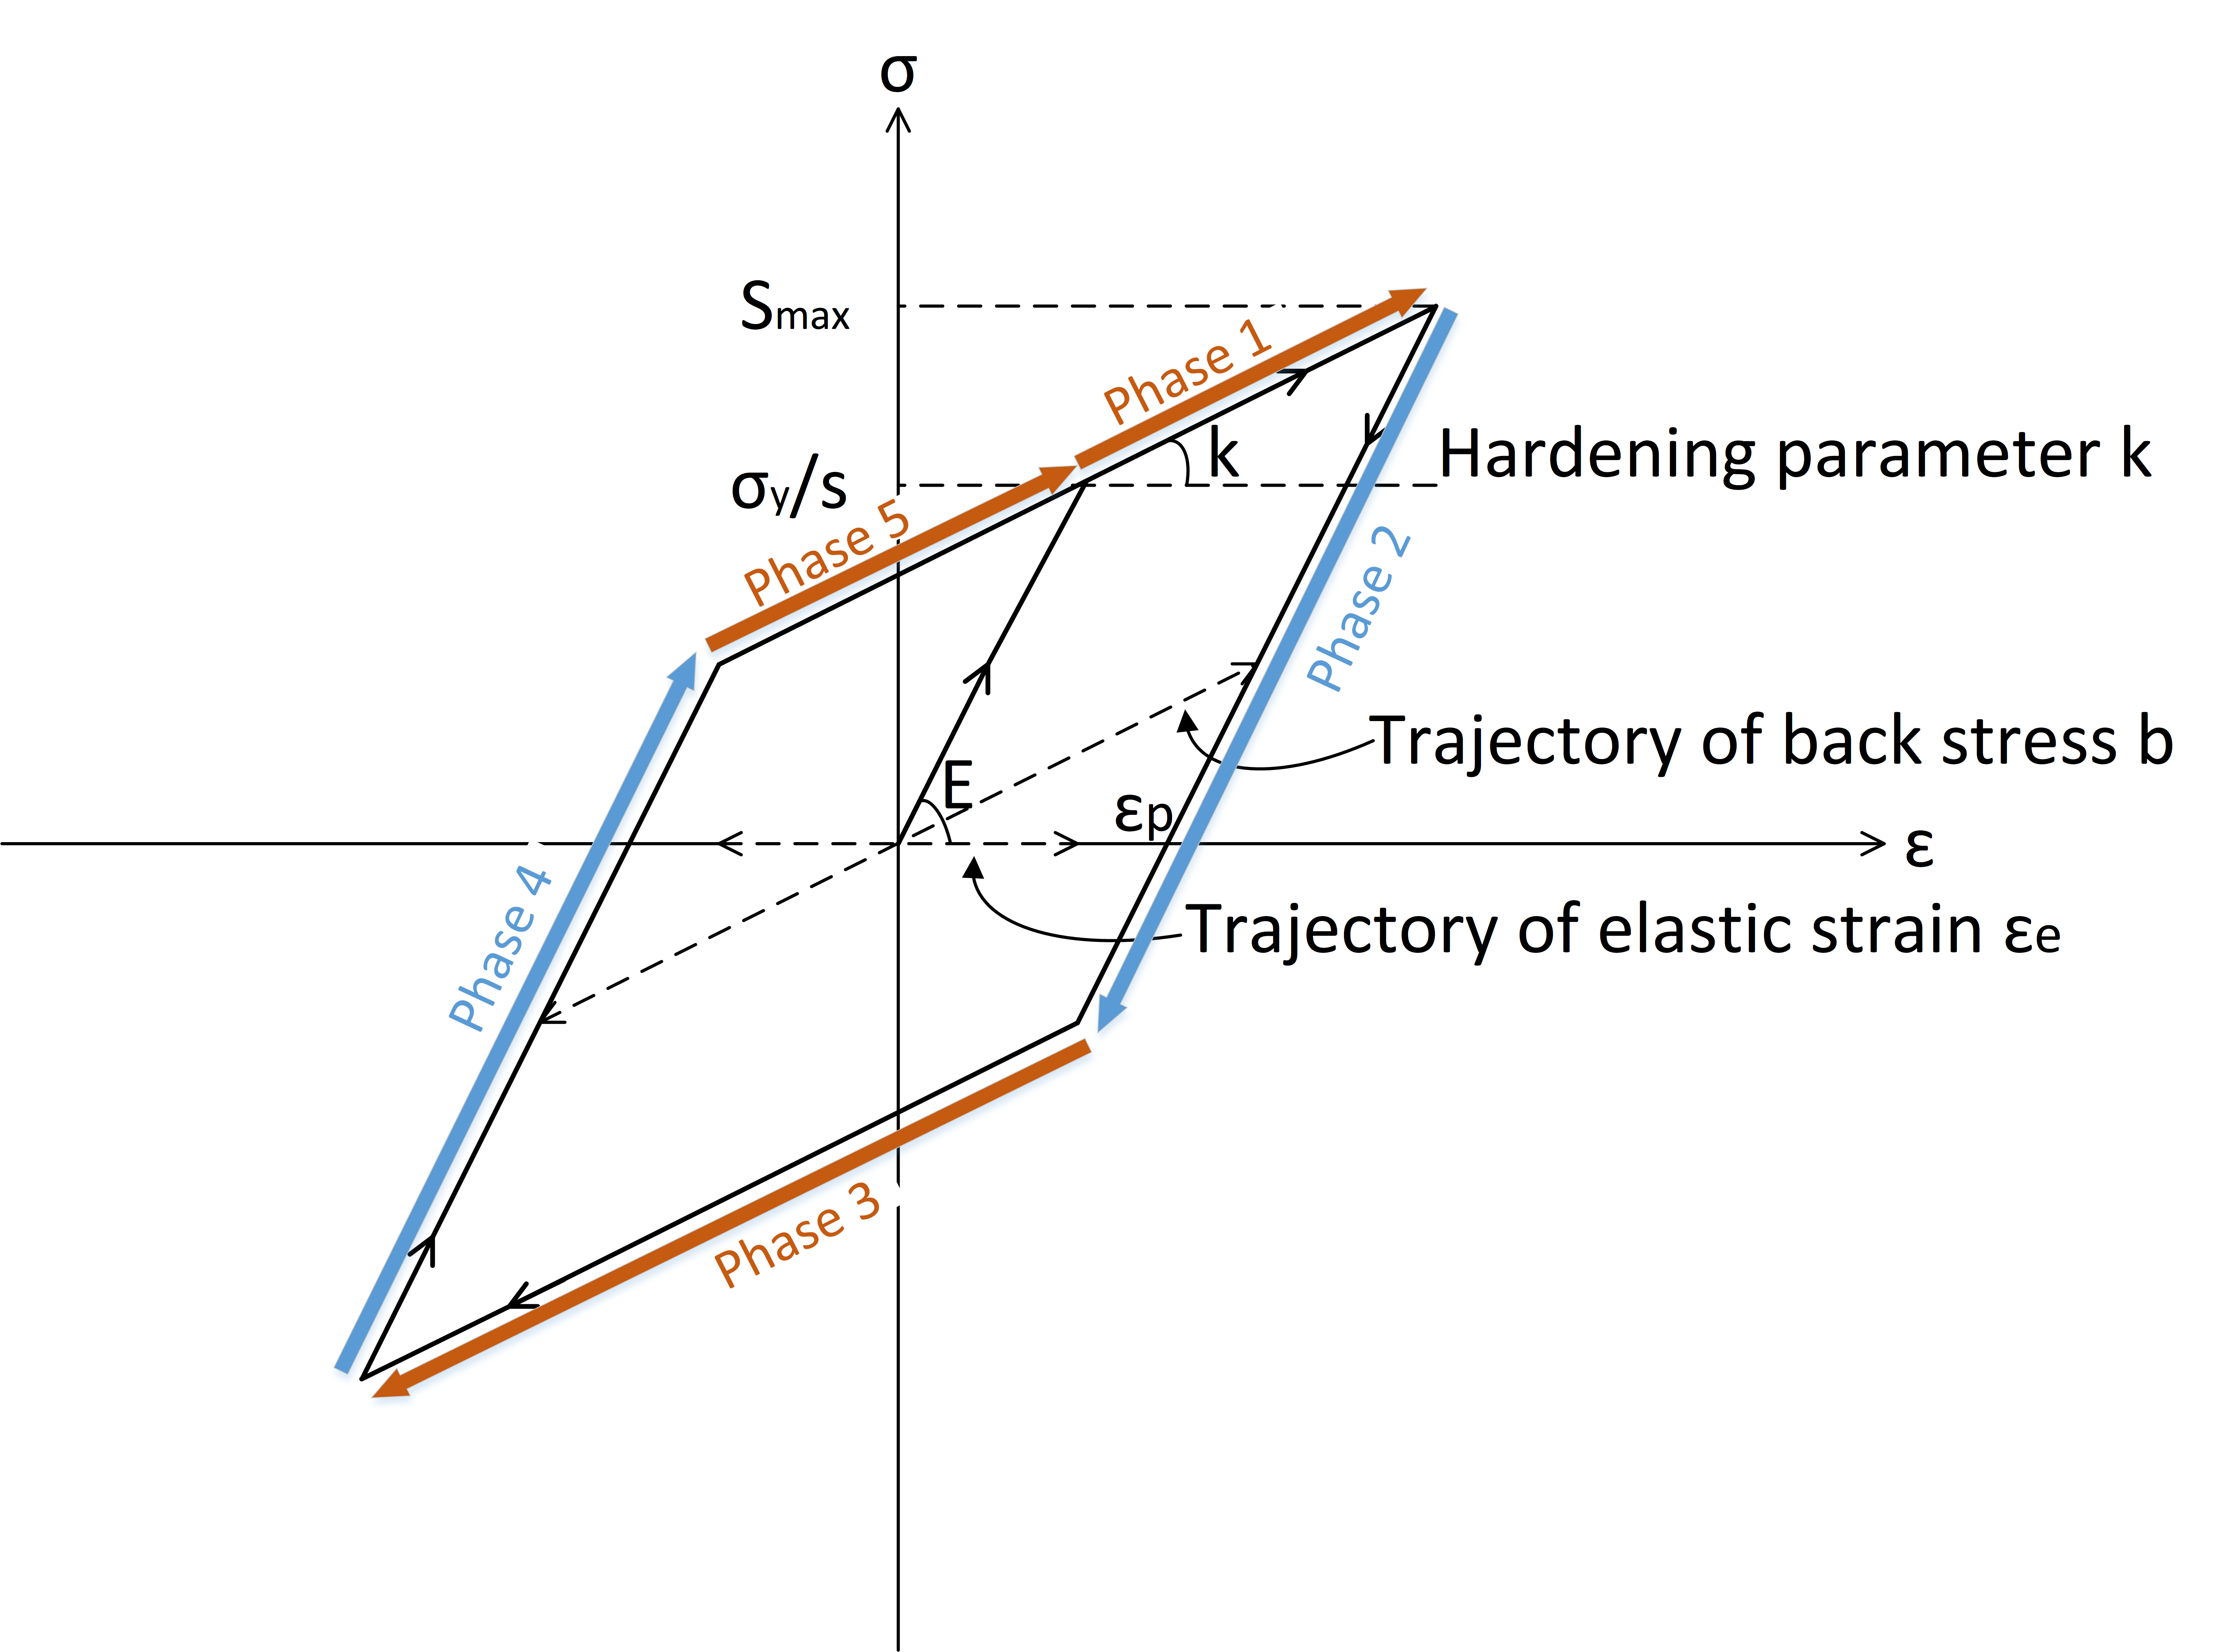
\includegraphics[width=0.9\textwidth]{figures//backstress.png} 
\caption{Uniaxial load with plastic dissipation}
\label{backstress}
\end{figure}

In phase 1, a direct analysis yields the energy dissipation at scale $s$:
\begin{equation}dW=(S-b)d\varepsilon^p=\dfrac{(E-k)(1+\nu) }{E(E+k\nu)}\dfrac{ \left(\sigma_y-\lambda \Sigma_H\right)}{s}\left(S_{a}-\dfrac{ \left(\sigma_y-\lambda \Sigma_H\right)}{s}\right).
\label{dw}
\end{equation}

A similar analysis yields $$dW(phase 1)=dW(phase 5)=\dfrac{1}{2}dW(phase 3).$$

We can then calculate  the local dissipated energy $W$  at point $M$ during one cycle by cumulating the input of all sub-scales plastic regime with their probabilities (\cite{zepeng}).
\begin{equation}
\begin{split}
W_{cyc}&=4\int_{ \left(\sigma_y-\lambda \Sigma_H\right) /S_{a}}^{\infty}dW(s,M,t)P(s)ds
\\&=4\int_{ \left(\sigma_y-\lambda \Sigma_H\right) /S_{a}}^{\infty}\dfrac{(E-k)(1+\nu) }{E(E+k\nu)}\dfrac{ \left(\sigma_y-\lambda \Sigma_H\right)}{s}\left(S_{a}-\dfrac{ \left(\sigma_y-\lambda \Sigma_H\right)}{s}\right)\left( \beta-1\right) s^{-\beta}ds
\\&=\dfrac{4(E-k)(1+\nu)\left( \beta-1\right) }{ E(E+k\nu)\beta\left( \beta+1\right) }\dfrac{S_{a}^{\beta+1}}{ \left(\sigma_y-\lambda \Sigma_H\right)^{\beta-1}}.
\end{split}
\label{eq:w}
\end{equation}

So we have a power law relationship between stress intensity and the dissipated energy per cycle.
\begin{equation}
W_{cyc}=C_1S_{a}^{\beta+1},
\label{eq.wcyc}
\end{equation}
with 
$$C_1=f(\lambda,\beta)=\dfrac{4(E-k)(1+\nu)\left( \beta-1\right) }{ E(E+k\nu)\beta\left( \beta+1\right)\left(\sigma_y-\lambda \Sigma_H\right)^{\beta-1} }.$$
If the dissipated energy accumulates until a failure value $W_0$, we can get directly the number of cycles to failure from Eq.\eqref{eq.wcyc} as:
\begin{equation}
N_{F}=\dfrac{W_0}{W_{cyc}}=\dfrac{W_0}{C_1}S_{a}^{-\beta-1}.
\label{eq.NFcyc}
\end{equation}
As for the time to failure in cyclic loading, it will be:
$$T_{F}=N_{F}t_{cyc}.$$
From Eq.\eqref{eq:w}, we then obtain that in uniaxial cyclic loading the model predicts as expected (Chapter \ref{chp:4}) a power law dependence of the number of cycles to failure in function of $S_{a}$.
However, experiments shows that the damage or the energy accumulation of a material evolves non-linearly in time and present a load dependent cycle (Chapter \ref{chp:4}). We should introduce below a method to handle such a nonlinearity.

\section{Nonlinearity of damage accumulation}
\label{sec:5.6}
\subsection{Energy approach with Chaboche law}
The Chaboche law (\cite{lemaitre1990mechanics}) is essentially a damage incremental law for cyclic loads with a deviatoric stress intensity ${A}_{\uppercase\expandafter{\romannumeral2}}$ and hydrostatic mean part $\Sigma_H$, defining the damage increase by:

\begin{equation}\delta D = \left( 1 -(1-D)^{\gamma+1}\right)^\alpha \left(\frac{{A}_{\uppercase\expandafter{\romannumeral2}} }{M(\sigma_H)\left( 1-D\right)}\right)^\gamma \delta N ,
\label{chabochemulti}
\end{equation} 

using an effective intensity ${A}_{\uppercase\expandafter{\romannumeral2}}^*={A}_{\uppercase\expandafter{\romannumeral2}}/\left( 1-D\right) $ evolving with damage $D$. And the mean stress effect is present both in exponential factor $\alpha$ and in denominator $M(\sigma_H)$.
$$\alpha=1 - a\left\langle \dfrac{\dfrac{1}{2}{A}_{\uppercase\expandafter{\romannumeral2}}-\sigma_{-1}M(\sigma_H) }{\sigma_{u} -{A}_{\uppercase\expandafter{\romannumeral2}}}\right\rangle,$$
$$M(\sigma_H) =M_0 \left(1-3c\sigma_{H,max}\right).$$

Eq.\eqref{chabochemulti} writes equivalently:
\begin{equation}\delta [1-(1-D)^{\gamma+1}]^{1-\alpha}=(1-\alpha)(\gamma+1)\left(\dfrac{{A}_{\uppercase\expandafter{\romannumeral2}} }{M(\Sigma_H)}\right)^\gamma \delta N=\dfrac{1}{N_F(\sigma)}\delta N.
\label{integration}
\end{equation}
Here $N_F(\sigma)$ denotes the number of cycles at intensity $\sigma$ to failure as obtained by integration of Eq.\eqref{integration} from $D=0$ to $D=1$. 

%
%The nonlinear damage incremental law using energy dissipation:
%\begin{equation}
%\begin{split}
%  \delta D &=\dfrac{\left( 1 -(1-D)^{\gamma+1}\right)^\alpha}{\left(1-D \right)^\gamma} \delta W
%  \\&= \dfrac{\left( 1 -(1-D)^{\gamma+1}\right)^\alpha}{\left(1-D \right)^\gamma} \dfrac{W_{cyc}\delta N}{W_0}
%  \\&= \dfrac{\left( 1 -(1-D)^{\gamma+1}\right)^\alpha}{\left(1-D \right)^\gamma} \dfrac{4(E-k)(1+\nu)\left( \beta-1\right) }{ E(E+k\nu)\beta\left( \beta+1\right) }\dfrac{S_{a}^{\beta+1}}{\left(\sigma_y-\lambda \Sigma_H\right)^{\beta-1}}\dfrac{\delta N}{W_0}.
%\end{split}
%\label{recoverchaboche}
%\end{equation} 
%
%We compare Eq.\eqref{chabochemulti} and Eq.\eqref{recoverchaboche}, in Chaboche model there is:
%$$\beta+1=\gamma. $$

Similar to Eq.\eqref{integration}, we define here the ``equivalent damage'' $\tilde{D}$(\figref{eq.Dhat}) :

\begin{equation}
\tilde{D}=1-(1-D)^{\gamma+1},
\label{eq.Dhat}
\end{equation}
with $D$ the damage variable introduced by Chaboche in its model to scale the stress intensity:
$${A}_{\uppercase\expandafter{\romannumeral2}} \longrightarrow \dfrac{{A}_{\uppercase\expandafter{\romannumeral2}}}{1-D}.$$

We have 

$\bullet$ $\tilde{D}=0$ when $D=0$ (undamaged material),

$\bullet$ $\tilde{D}=1$ when $D=1$ (failure of material),	

and a nonlinear relation in between as in \figref{fig.Dhat}:
$$\delta\tilde{D}=\left(\gamma+1 \right)\left( 1-D\right)^\gamma \delta D.$$	
\begin{figure}
\centering
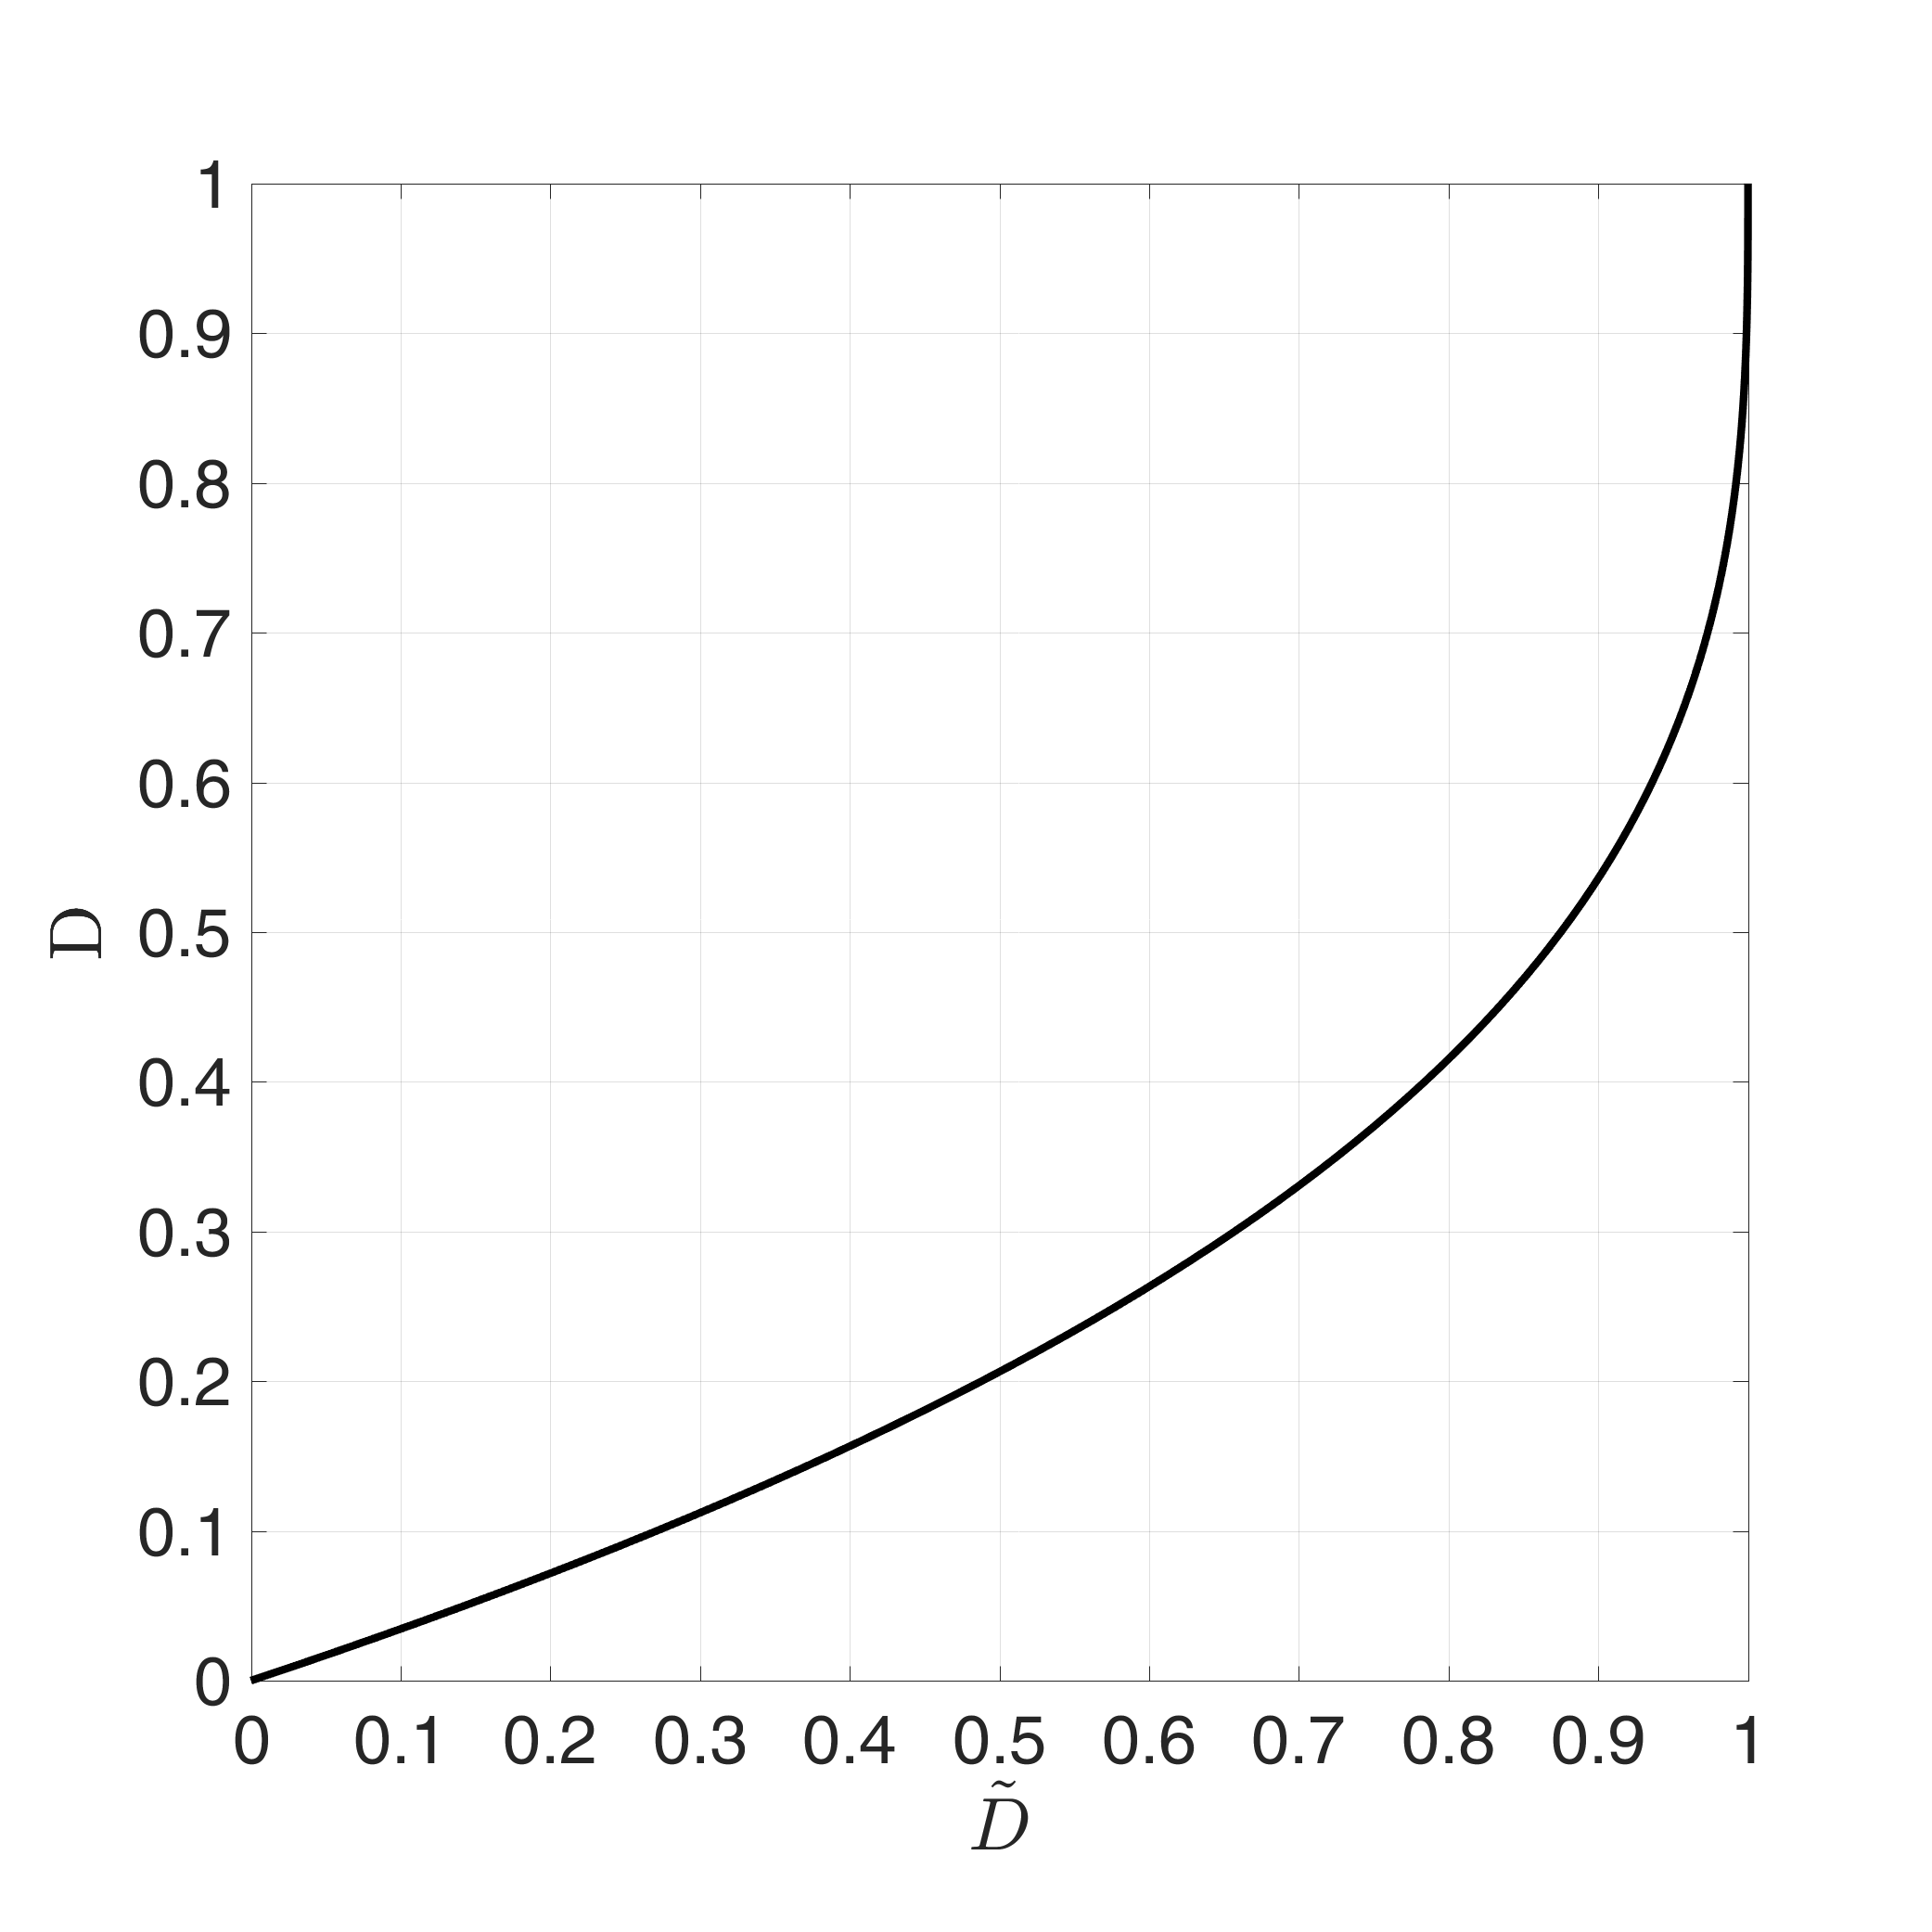
\includegraphics[width=0.6\textwidth]{figures//Dhat.png} 
\caption{The relation between $\tilde{D}$ and $D$ when $\gamma=2$}
\label{fig.Dhat}
\end{figure}

Change of damage measure $\tilde{D} = 1 - (1-D)^{\gamma+1}$ makes the evolution \eqref{chabochemulti} explicit. It writes
\begin{equation}
\dfrac{d\tilde{D}}{dN} = c_D {\tilde{D}}^\alpha \left(\dfrac{{A}_{\uppercase\expandafter{\romannumeral2}}}{M(\Sigma_{H})} \right) ^\gamma,
\label{eq.diffchaboche}
\end{equation}
yielding after integration from $\tilde{D}=0$ to $\tilde{D}=1$  a number of cycles to fatigue at constant load given by
$$
N_F =\dfrac{1}{(1-\alpha)}\left(\dfrac{{A}_{\uppercase\expandafter{\romannumeral2}}}{M(\Sigma_{H})} \right) ^{-\gamma}.
$$

This method as written requires cycle counting which is difficult and technical for complex load histories. In addition, it allows only a limited influence of multiaxiality.


Now in our model we use the same growth rule as in Chaboche in cyclic load regime, but replace stress intensity by multiscale dissipated energy  in Eq.\eqref{eq.diffchaboche}, which removes cycle counting.

The evolution \eqref{eq.diffchaboche} then writes
$$
\dfrac{d\tilde{D}}{dt} ={\tilde{D}}^\alpha \dot{W}/W_0,
$$
or in a differential form
\begin{equation}
d \tilde{D}=\tilde{D}^\alpha\dfrac{d W}{W_0}=\tilde{D}^\alpha\dfrac{W_{cyc}d N}{W_0}.
\label{eq.DWcyc}
\end{equation}

The replacement of $d W$ by $W_{cyc}dN$ is only introduced to handle cyclic loadings if they occur. The number of cycles to failure in constant loading case, obtained by integrating $\tilde{D}$ from $\tilde{D}_0$ to 1 is then:
$$N_F=\dfrac{W_0}{\left( 1-\alpha\right)W_{cyc} }\left( 1-D_0^{1-\alpha}\right) .$$
With initial damage $D_0=0$, we finally get with our proposed expression Eq.\eqref{eq.wcyc} of cyclic energy dissipation:
\begin{equation}
N_F=\dfrac{W_0}{\left( 1-\alpha\right)W_{cyc} }=\dfrac{W_0}{(1-\alpha)C_1}S_{a}^{-\beta-1}.
\label{eq.NFWcyc}
\end{equation}

From Eq.\eqref{eq.NFWcyc}, we see $(-\beta-1)=-\gamma$ is related to the slops in S-N curve and that $\dfrac{W_0}{(1-\alpha)C_1}$ defines the number of cycles to failure.
\subsection{Sequence effect}

Experiments show fatigue tests started with high stress then change to low stress has less fatigue life than the combination of high stress life proportion plus the low one. This phenomenon of sequence effect is load history dependent, so we need a stress induced parameter to describe it. 

This is done in Chaboche  with three ingredients:

\begin{enumerate} 
\vspace{6pt}
\item a damage sensitive effective stress: 
$$\sigma_D^{eff} = J_2(\uline{\uline{\Sigma}})/(1-D)={A}_{\uppercase\expandafter{\romannumeral2}}/(1-D);$$

\vspace{6pt}

\item a $(\sigma_D^{eff})^\gamma$ controlled  law for damage growth
$$\dfrac{dD}{dN} =c_\gamma {\tilde{D}}^\alpha (\sigma_D^{eff})^\gamma;$$

\vspace{6pt}

\item  a load dependence of exponent $\alpha$ (from $1$ at zero load to $0$ at large loads). In Chaboche model, the proposition of $\alpha$ is
\begin{equation}
\alpha = 1 - a\left\langle \frac{ \sigma_{eq}-\sigma_{fatigue}}{ \sigma_{u} - \sigma_{eq}}\right\rangle
\label{eq.alpchaboche}
\end{equation}
in order to recover the proper high-low sequencing effect.
\end{enumerate}

Many fatigue damage accumulation models are based on the two level loading experiments which is one of the basic random loading analysis. To facilitate the validation and interpretation of an $\alpha$ dependence on stress we will also use two-stress level loading, the specimen is firstly loaded at stress $\Sigma_1$ for $T_1$ cycles and then at stress $\Sigma_2$ for $T_2$ cycles until failure. We can then observe if the experimental results are satisfactory.

During a loading time $T_1$, we  cycle  from $\tilde{D}=0$ to $\tilde{D}= \tilde{D}_1$. By integrating Eq.\eqref{eq.DWcyc} of our proposed approach, we get:
\begin{equation}
\left( 1-\tilde{D}_1\right) ^{1-\alpha_1}=\dfrac{T_1}{T_{F1}},
\label{23a}
\end{equation}
with $T_{F1}$ the time to failure with this loading.

Then we cycle from  ${\tilde D}={\tilde D}_1$ to failure ${\tilde D}=1$, which yields
\begin{equation}
1-\left( 1-\tilde{D}_1\right)^{1-\alpha_2}=\dfrac{T_2}{T_{F2}}.
\label{23b}
\end{equation}

From Eq.\eqref{23a} and Eq.\eqref{23b}, after elimination of $\left( 1-D_1\right)$ we get:
\begin{equation} 
\dfrac{T_2}{T_{F2}} =1-\left( \dfrac{T_1}{T_{F1}}\right) ^\eta,
\label{eq.sequence}
\end{equation}
with
\begin{equation}
\eta=\dfrac{1-\alpha_2}{1-\alpha_1}.
\label{eq.eta}
\end{equation}

In the case of high-low loading sequence we have $\Sigma_1>\Sigma_2$,  which gives $\alpha_1<\alpha_2$, so it comes to:
$$\eta=\frac{1-\alpha_2}{1-\alpha_1}<1 \implies
\frac{T_2}{T_{F2}}=1-\left( \frac{T_1}{T_{F1}}\right) ^\eta<1-\frac{T_1}{T_{F1}} \implies
\frac{T_1}{T_{F1}}+\frac{T_2}{T_{F2}}<1.$$

The $\alpha$ dependence on stress intensity does therefore predict a sequencing effect where a low loading sequence following a high one will reduce the life of the structure if $\alpha$ decreases when the load increases.

To get the same effect in our construction, we propose here to introduce $s_{min}$, which is the minimum scale that experiences plastic dissipation thus causes energy loss:
\begin{equation}
s_{min}=\dfrac{\left(\sigma_y-\lambda \Sigma_H\right)}{S_{a}}.
\label{eq.smin}
\end{equation}

We propose a load dependent $\alpha$ through $s_{min}$. Possible choice
of $\alpha$ is expressed as Eq.\eqref{eq.alpha}:
\begin{equation}
\alpha=1-a\left( \dfrac{\frac{1}{s_{min}}}{1-\frac{1}{s_{min}}} \right) .
\label{eq.alpha}
\end{equation}

There is no notion of fatigue limit in our model, $\sigma_{faigue}=0$. The intensity of loading
$$\frac{ \sigma_{eq}-\sigma_{fatigue}}{ \sigma_{u} - \sigma_{eq}}= \frac{ 1}{\frac{\sigma_{u}}{\sigma_{eq}} -1}$$
is measured by 
$$\left( \dfrac{\frac{1}{s_{min}}}{1-\frac{1}{s_{min}}}\right) =\left(s_{min}-1 \right) ^{-1}.$$
This means that we measure the distance of load to ultimate failure by local variable $s_{min}$ through 

$$\frac{\sigma_{u}}{\sigma_{eq}} -1 \longrightarrow \left( s_{min}-1\right)  $$


We can see from \figref{fig.sequence} that with our proposition, cycling $1$ for fifty percent of its failure time leaves a reserve before failure to cycling $2$ of much less than fifty percent. To conclude, the cumulative damage under high-low loading sequence, as we deduced, has the addition of partial lives less than unit. Similarly, the cumulative damage under low-high loading sequence has addition of partial lives more than 1:
$$\frac{T_1}{T_{F1}}+\frac{T_2}{T_{F2}}>1.$$
The curve in both cases is depicted in \figref{fig.sequence}.
\begin{figure}[!h]
\centering
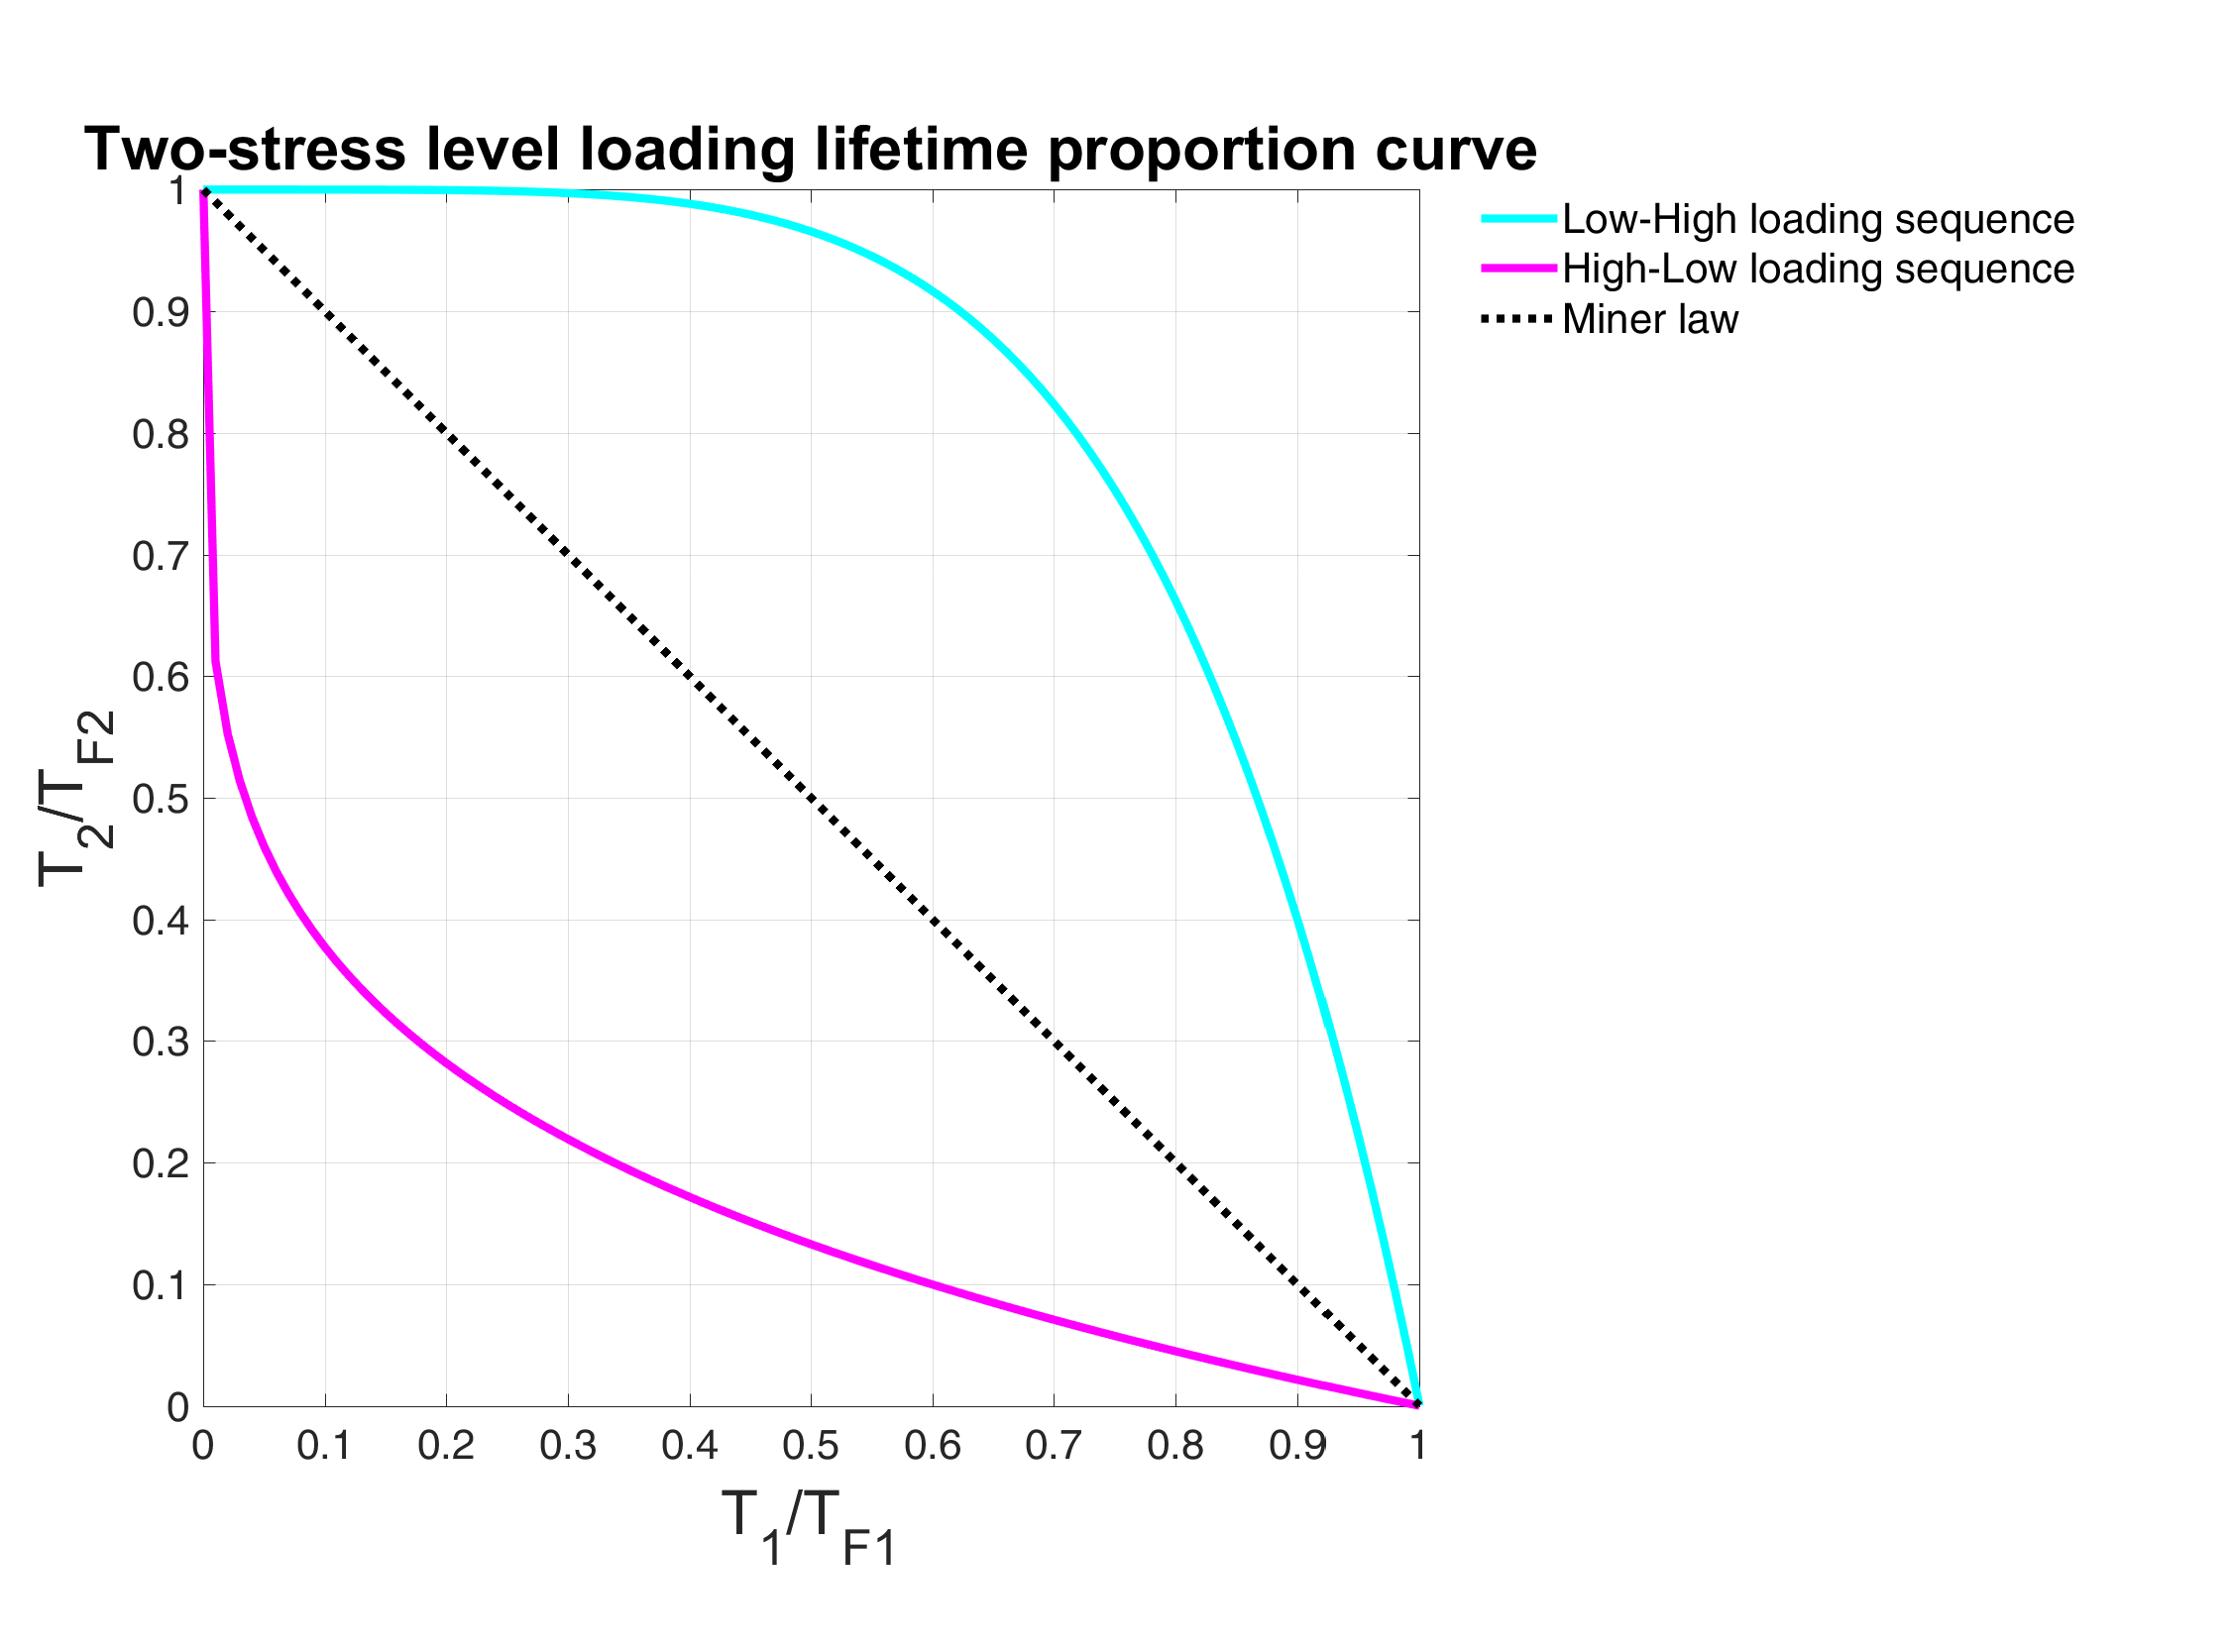
\includegraphics[width=0.8\textwidth]{figures//sequence.png} 
\caption{High to low and low to high loading sequence comparison in 4-point bending($F_{low}=5000 N, F_{high}=30000 N, Radius=0.2m, \Sigma_u=1.67E8$), with the proposed damage accumulation law (Eq.\eqref{eq.DWcyc}) induced equation Eq.\eqref{eq.sequence} and Chaboche type $\alpha$ (Eq.\eqref{eq.alpchaboche}) containing Crossland criterion}
\label{fig.sequence}
\end{figure}
For constant two-level stress loading, $\alpha_1=\alpha_2$, the Chaboche law returns to the Miner rule when $F_{low}=F_{high}$ where:
$$\frac{T_1}{T_{F1}}+\frac{T_2}{T_{F2}}=1.$$

\newpage
\subsection{The final model}
\label{sec:5.6.3}
In summary, our damage based fatigue life criterion using a damage evolution governed by a multiscale plastic energy dissipation, has four ingredients.
\begin{itemize}
\item  a scale dependent yield limit $$\frac{1}{s} (\sigma_y- \lambda \Sigma_H^{macro})$$ associated to a microscopic plastic evolution governed by the standard plastic evolution laws Eq.\eqref{eq.mesostress} - Eq.\eqref{eq.plasticflow};

\vspace{6pt}	

\item a multiscale plastic energy dissipation obtained by summing plastic dissipation across our power law scale distribution
\begin{equation}
\dot{W}(M,t)=\int_{s=1}^{\infty}\left(\uline{\uline{S}}-\uline{\uline{b}} \right) (s,M,t):\uline{\uline{\dot{\varepsilon}}}^p(s,M,t) s^{-\beta}ds;
\label{eq.final2}
\end{equation}

\vspace{6pt}	

\item a load intensity sequencing effect that we have represented by the formula : 
\begin{equation}
1 - \alpha = a (s_{min}-1)^{-f};
\label{eq.final3}
\end{equation}

\vspace{6pt}	

\item a exponential damage evolution law with load dependent exponent $\alpha$ given by the above formula and coefficient $\dot{W}/W_0$ governed by the multiscale plastic dissipation rate: 
\begin{equation}
\dfrac{d\tilde{D}}{dt} ={\tilde{D}}^\alpha \dot{W}/W_0.
\label{eq.final4}
\end{equation}
\end{itemize}

In this model we have five independent coefficients in addition to the construction of the local plastic model Eq.\eqref{eq.mesostress} - Eq.\eqref{eq.plasticflow} :

\begin{enumerate}
\item reference density of damage energy : $W_0$ (in MPa)

\item mean stress effect coefficient : $\lambda$
\item slope of SN curve : $\beta+1$

\item sensitivity to load intensity $a$. 
\item exponent in the load sequence effect $f$. 
\end{enumerate}

\newpage
\section{Numerical strategy}
\label{sec:5.7}
\subsection{Scale discretization}
We now need to propose a practical implementation strategy for our final model of section \ref{sec:5.6.3}.Our first approach takes one cycle as unit time. We compute analytically by Eq.\eqref{eq:w} the energy dissipation at each scale during this cycle. The method is valid for simple loading history and which includes the integration on all weakening scales. The damage $\tilde{D}$ is then accumulated after each cycle by numerical integration of Eq.\eqref{eq.final4} until we get to the fatigue limit of $\tilde{D}=1$.

However, there are certain limitations of this method. Firstly we need a load history decomposition in cycles. Secondly in real life the perfect close loop cycle is hardly applicable. Finally, we need to approximate $\alpha$  by its average value per cycle which is computed numerically and can not be done analytically.

Thus we propose in a more general method which can be integrated by a step by step strategy. We compute numerically the dissipation at different scales using an implicit Euler time integration of the constitutive laws of section \ref{sec:5.4.4}. After which we make a numerical integration on different scales. Then we can update the damage and go to next time step. 

Instead of doing the scale integration directly which can be difficult for complex loading, the Gaussian Quadrature rule with Legendre points is used to give the value of local dissipated energy rate. To use the Gaussian quadrature rule the limit range of integral must be from $-1$ to $1$, while the total dissipated energy  is expressed by integrating all the weakening scale $s$ ranging from 1 to infinity with their occurrence probabilities:
$$\dot{W}=\int_{1}^{\infty}\dot{w}(s) (\beta-1)(s)^{-\beta}ds.$$

\noindent
To change the limit range of integral from $[1,\infty]$ to $[1,0]$ we take as new integration variable
$u(s)= s^{1-\beta}$. Therefore the dissipated energy summed on all scales is:
\begin{equation}
\begin{split}
\dot{W}&=\int_{1}^{\infty}\dot{w}(s) (\beta-1)(s)^{-\beta}ds
\\&=\int_{0}^{1}\dot{w}\left( u^{\frac{1}{1-\beta}}\right)du
\\&=\frac{1}{2}\int_{-1}^{1}\dot{w}\left[  \left( \frac{x+1}{2}\right) ^{\frac{1}{1-\beta}}\right] dx
\end{split}
\label{allscale}
\end{equation}
given $u=\dfrac{x+1}{2}$. So the dissipated energy rate integrated over all scales takes the form of Eq.\eqref{allscalerate}:
\begin{equation}
\dot{W}=\frac{1}{2}\int_{-1}^{1}\dot{w}\left[  \left( \frac{x+1}{2}\right) ^{\frac{1}{1-\beta}},t\right] dx\approx\frac{1}{2}\sum_{i}\omega_i\dot{w}\left[  \left( \frac{x_i+1}{2}\right) ^{\frac{1}{1-\beta}},t\right],
\label{allscalerate}
\end{equation}
where $\omega_i$ and $x_i$ are respectively the weights and nodes of the Gauss Legendre integration rule used for the numerical integration.  In this work, we used a 64 points Gaussian Legendre integration rule (\cite{Legendre}) with $s_i=\left( \dfrac{x_i+1}{2}\right) ^{\frac{1}{1-\beta}}$ being the associated scale.

\subsection{Calculation of local plastic dissipation}
\label{sec:5.4.4}
The material could be both in elastic and plastic regime depending on the considered scale. To be more elaborate, we reuse the fundamental equations in different regimes. At scale $s$, we have a dissipation rate given by:
$$\dot{w}(s)=\left( \uline{\uline{S}}-\uline{\uline{b}}\right):\dot{\uline{\uline{\varepsilon}}}^p, $$
which differs between plastic and elastic regime.

\vspace{6pt}
\noindent
\textbf{Elastic regime:}

\vspace{6pt}
\noindent
There we have
plastic strain rate
$\dot{\uline{\uline{\varepsilon}}}^p=0$, back stress rate $\dot{\uline{\uline{b}}}=0$ and deviatoric stress rate $\dot{\uline{\uline{S}}}=dev\dot{\uline{\uline{\Sigma}}}$, leading to
$$\dot{\uline{\uline{S}}}-\dot{\uline{\uline{b}}}=dev\dot{\uline{\uline{\Sigma}}},$$ 
meaning
$$\left( \uline{\uline{S}}-\uline{\uline{b}}\right) (t+dt)=\left( \uline{\uline{S}}-\uline{\uline{b}}\right) (t)+dev\dot{\uline{\uline{\Sigma}}}dt.$$
At each time step we define a trial stress:
\begin{equation}
\left( \uline{\uline{S}}-\uline{\uline{b}}\right)_{trial}:=\left( \uline{\uline{S}}-\uline{\uline{b}}\right)(t+dt).
\label{trial}
\end{equation}
We are in elastic regime at scale $s$ as long as we satisfy

\begin{equation}
\left| \left|  \uline{\uline{S}}-\uline{\uline{b}}\right| \right| _{trial}\leqslant\left( \sigma_y-\lambda \Sigma_H\right)/s.
\label{eq.trialelastic}
\end{equation}

\vspace{6pt}
\noindent
\textbf{Plastic regime:}
\vspace{6pt}

\noindent
When we leave elastic regime at scale s, i.e. when the above inequality Eq.\eqref{eq.trialelastic} is violated, we have:
\begin{numcases}{}
\dot{\uline{\uline{\varepsilon}}}^p=\xi\dfrac{\uline{\uline{S}}-\uline{\uline{b}}}{\left| \left|\uline{\uline{S}}-\uline{\uline{b}}\right| \right|}, \xi>0, & plastic   flow, \label{plasticflow}
\\
\left| \left|\uline{\uline{S}}-\uline{\uline{b}}\right| \right|= \left(\sigma_y-\lambda \Sigma_H\right)/s, & yield   limit,\label{yieldlimit}
\\
\left( \uline{\uline{S}}-\uline{\uline{b}}\right) :\left( \dot{\uline{\uline{S}}}-\dot{\uline{\uline{b}}}\right) =0, & yield   limit   time invariance,
\\
\dot{\uline{\uline{b}}}=\dfrac{kE}{E-k}\dot{\uline{\uline{\varepsilon}}}^p, & kinematic   hardening  rule, \label{kinematichardening}
\\
\dot{\uline{\uline{S}}}=dev\dot{\uline{\uline{\Sigma}}}-\dfrac{E}{1+\nu} \dot{\uline{\uline{\varepsilon}}}^p, & localisation  rule. \label{localisation}
\end{numcases}

In all cases, we get by integrating Eq.\ref{localisation}, Eq.\ref{kinematichardening} with the use of Eq.\ref{plasticflow}.
\begin{equation}
\left( \uline{\uline{S}}-\uline{\uline{b}}\right) (s,t+dt)=\dfrac{\left( \uline{\uline{S}}-\uline{\uline{b}}\right)_{trial} (s,t+dt)}{1+\eta},
\end{equation}

and because of the yield condition Eq.\ref{yieldlimit}, we have
 $$\eta=max\left\lbrace \underbrace{0}_{elastic\; regime}, \underbrace{\dfrac{\left| \left|\uline{\uline{S}}-\uline{\uline{b}}\right| \right|_{trial}}{ \left(\sigma_y-\lambda \Sigma_H\right)/s}-1}_{plastic \; regime\; when\; this\; number\; is\; positive}\right\rbrace, $$

That is to say, when the structure is in elastic regime at time $t$ and scale $s$, we have $\left( \uline{\uline{S}}-\uline{\uline{b}}\right)(s,t)=\left( \uline{\uline{S}}-\uline{\uline{b}}\right)_{trial} (s,t)$. Otherwise, if  the norm of $\left( \uline{\uline{S}}-\uline{\uline{b}}\right)_{trial} (s,t)$ is greater than the local yield limit $ \left(\sigma_y-\lambda \Sigma_H\right)/s$, $\left( \uline{\uline{S}}-\uline{\uline{b}}\right)(s,t)$ will be projected on the yield limit. 

Knowing the distinction between elastic and plastic regime under multiple scales, we compute the general expression of the dissipated energy rate at scale $s$.
\begin{equation}
\dot{w}(s)=\left( \uline{\uline{S}}-\uline{\uline{b}}\right) :\dot{\uline{\uline{\varepsilon}}}^p=\gamma\dfrac{  \left(\sigma_y-\lambda \Sigma_H\right)}{s}.
\label{w}
\end{equation}

From Eq.\eqref{eta} and Eq.\eqref{eta2} in annex, we get:

\begin{equation}
	\begin{split}
		E\gamma dt&=\left\langle \left| \left|\uline{\uline{S}}-\uline{\uline{b}}\right| \right|_{trial}-\dfrac{ \left(\sigma_y-\lambda \Sigma_H\right)}{s}\right\rangle /\left(\dfrac{1}{1+\nu}+\dfrac{k}{E-k} \right)
		\\&=\left\langle \left| \left|\uline{\uline{S}}-\uline{\uline{b}}\right| \right|_{trial}-\dfrac{ \left(\sigma_y-\lambda \Sigma_H\right)}{s}\right\rangle\dfrac{(E-k)(1+\nu) }{(E+k\nu)},
	\end{split}
	\label{gamma}
\end{equation}
where $\langle$ $\rangle$ is Macaulay bracket symbol defined as $\langle m\rangle=0$ if $m\leqslant0$, otherwise $\langle m\rangle=m$. Thus the dissipated energy rate only depends on the evolution of the variable $\left( \uline{\uline{S}}-\uline{\uline{b}}\right)$, which must therefore be mentioned during the whole cycle under study.

We replace $\gamma$ deduced from Eq.\eqref{gamma} in Eq.\eqref{w} to give the expression of local energy dissipation rate at scale $s$:
\begin{equation}
\dot{w}(s)dt=\dfrac{(E-k)(1+\nu) }{E(E+k\nu)}\left\langle  \left| \left|\uline{\uline{S}}-\uline{\uline{b}}\right| \right|_{trial}-\dfrac{ \left(\sigma_y-\lambda \Sigma_H\right)}{s}\right\rangle \dfrac{ \left(\sigma_y-\lambda \Sigma_H\right)}{s}.
\label{dW}
\end{equation}

With Eq.\eqref{allscalerate}, the final expression of energy dissipation $W$ during time step $dt$ writes:

\begin{equation}
\begin{split}
W&=\dot{W}dt
\\&=\frac{1}{2}\sum_{i}\omega_i\dot{w}\left[  \left( \frac{x+1}{2}\right) ^{\frac{1}{1-\beta}}\right]dt
\\&=\dfrac{(E-k)(1+\nu) }{2E(E+k\nu)}\sum_{i}\omega_i\left\langle  \left| \left|\uline{\uline{S}}-\uline{\uline{b}}\right| \right|_{trial}-\dfrac{\left(\sigma_y-\lambda \Sigma_H\right) }{\left( \dfrac{x_i+1}{2}\right) ^{\frac{1}{1-\beta}}}\right\rangle \dfrac{\left(\sigma_y-\lambda \Sigma_H\right) }{\left( \dfrac{x_i+1}{2}\right)^{\frac{1}{1-\beta}}}.
\end{split}
\label{finaldw}
\end{equation}

The mean stress effect term in Chaboche model is $s_{-1}\left(1-3\dfrac{\sigma_H}{\sigma_u} \right)$, where the fatigue limit at zero mean stress $s_{-1}$ is reduced in the presence of $\sigma_H$. In our model, the yield limit decreases with positive mean stress. Because of the presence of the term $\lambda \Sigma_H$ which will be positive when $\Sigma_H$ is positive. In Eq.\ref{finaldw}, the coefficient $\lambda$ can change values if $\Sigma_H$ changes sign (see section \ref{sec:5.4.3}).


\subsection{Damage integration algorithm}

Numerically the  change of $\alpha$ is extremely nonlinear with time. From \figref{fig.alpmean} we can see the mean value of $\alpha$ depends on loading pattern. 

\begin{figure}[!h]
	\centering
	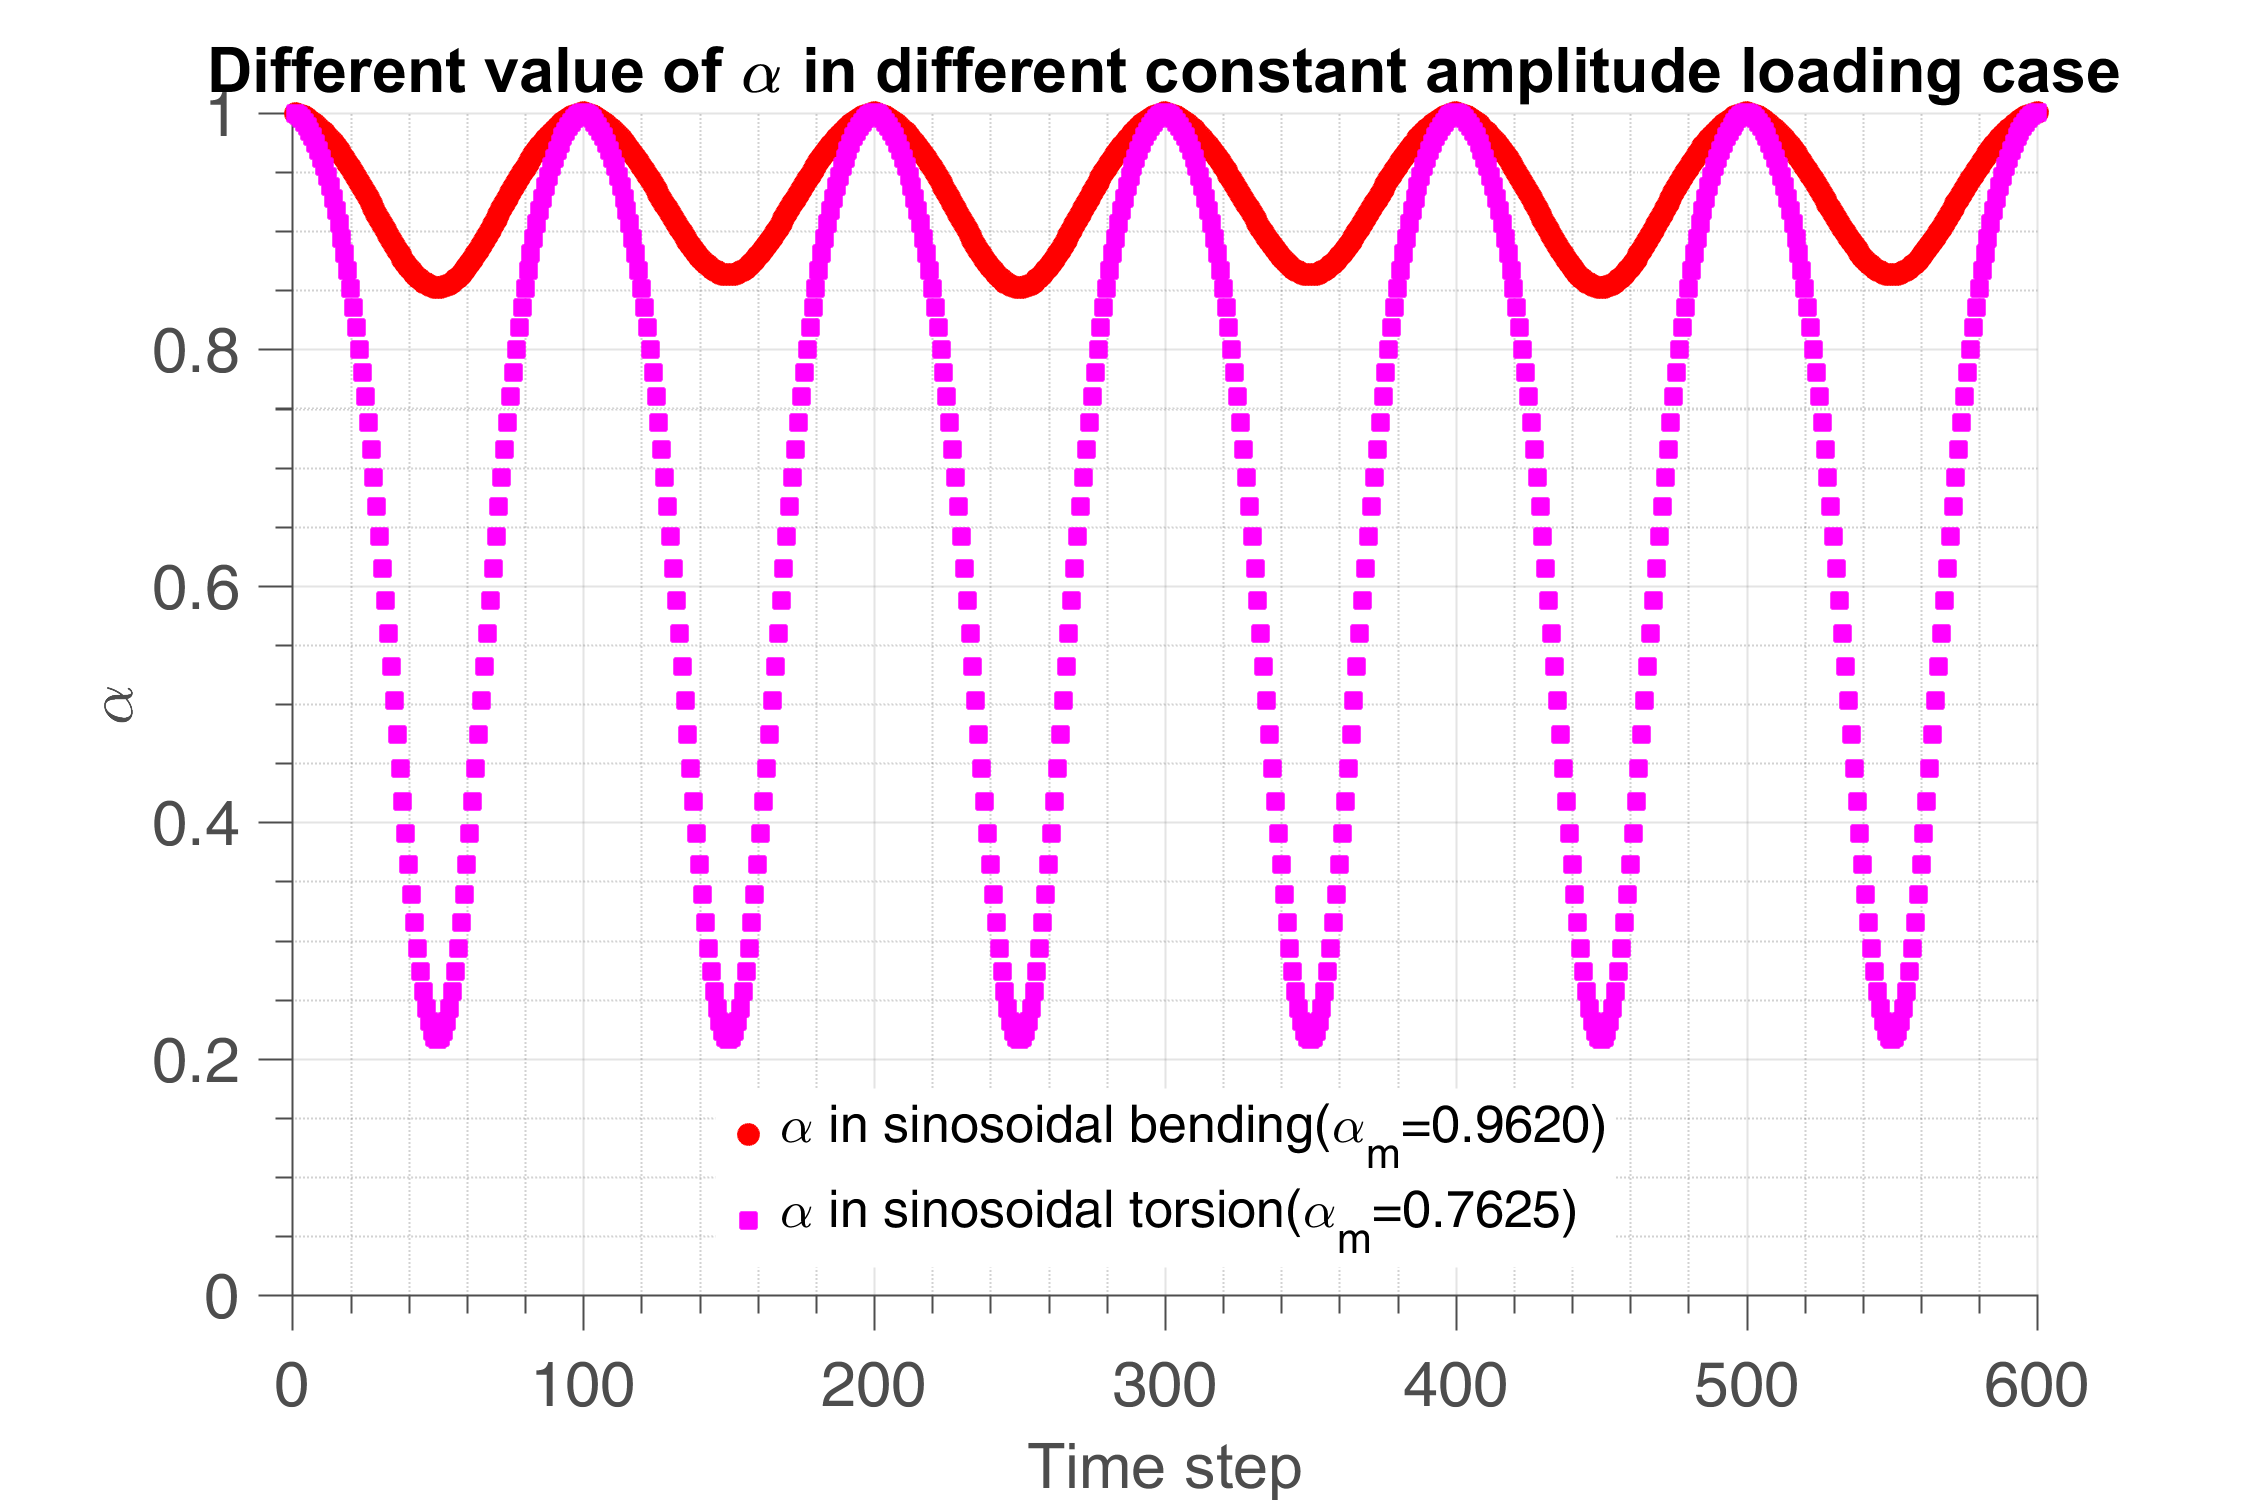
\includegraphics[width=0.8\textwidth]{figures//alp_mean_methods.png} 
	\caption{The evolution of $\alpha$ in bending and torsion with $\Sigma_y=1080 MPa$, $\Sigma_{bending}=\Sigma_{torsion}=500 MPa$, $a=0.3$ and $200$ time steps in one cycle}
	\label{fig.alpmean}
\end{figure}


Because of the possible large variations in time  of $\alpha$, the evolution problem in damage is very nonlinear and thus, one needs to develop and validate an improved numerical time integration strategy at least  for two specific cases: the constant amplitude case and the random load case.

We propose in constant amplitude load with very small evolution of damage per cycle to numerically calculate $W_{cyc}$ and the mean values of $\alpha$ through one cycle or several cycles(out-of-phase condition) and apply the result to life prediction by using  Eq.\eqref{eq.NFWcyc}:
\begin{equation}
N_F= \dfrac{W_0}{\left( 1-\alpha_m\right) W_{cyc}},
\label{eq.cycNF}
\end{equation}
which is obtained by direct integration of our damage law assuming time uniform dissipation in one cycle and frozen $\alpha$.
In this way the numerical cost is not as high as for the numerical implementation of all the loading points in random loading case. Because of the symmetrical shape of the evolution of $\alpha$, numerically the mean value of $\alpha$ does not strongly depend on the number of steps per cycle. In the verification process we have compared $100\sim1000$ time steps per cycle (\figref{fig.sn-num-ana}). 

For complex cyclic load cases, the idea is to accurately compute the history of plastic dissipation during one cycle (multiscale calculation with time refinement), and to use this precomputed result in the time integration of the scalar damage evolution law with a time stepping which is adapted to the time variation of $\alpha$. 

\begin{figure}[!h]
	\centering
	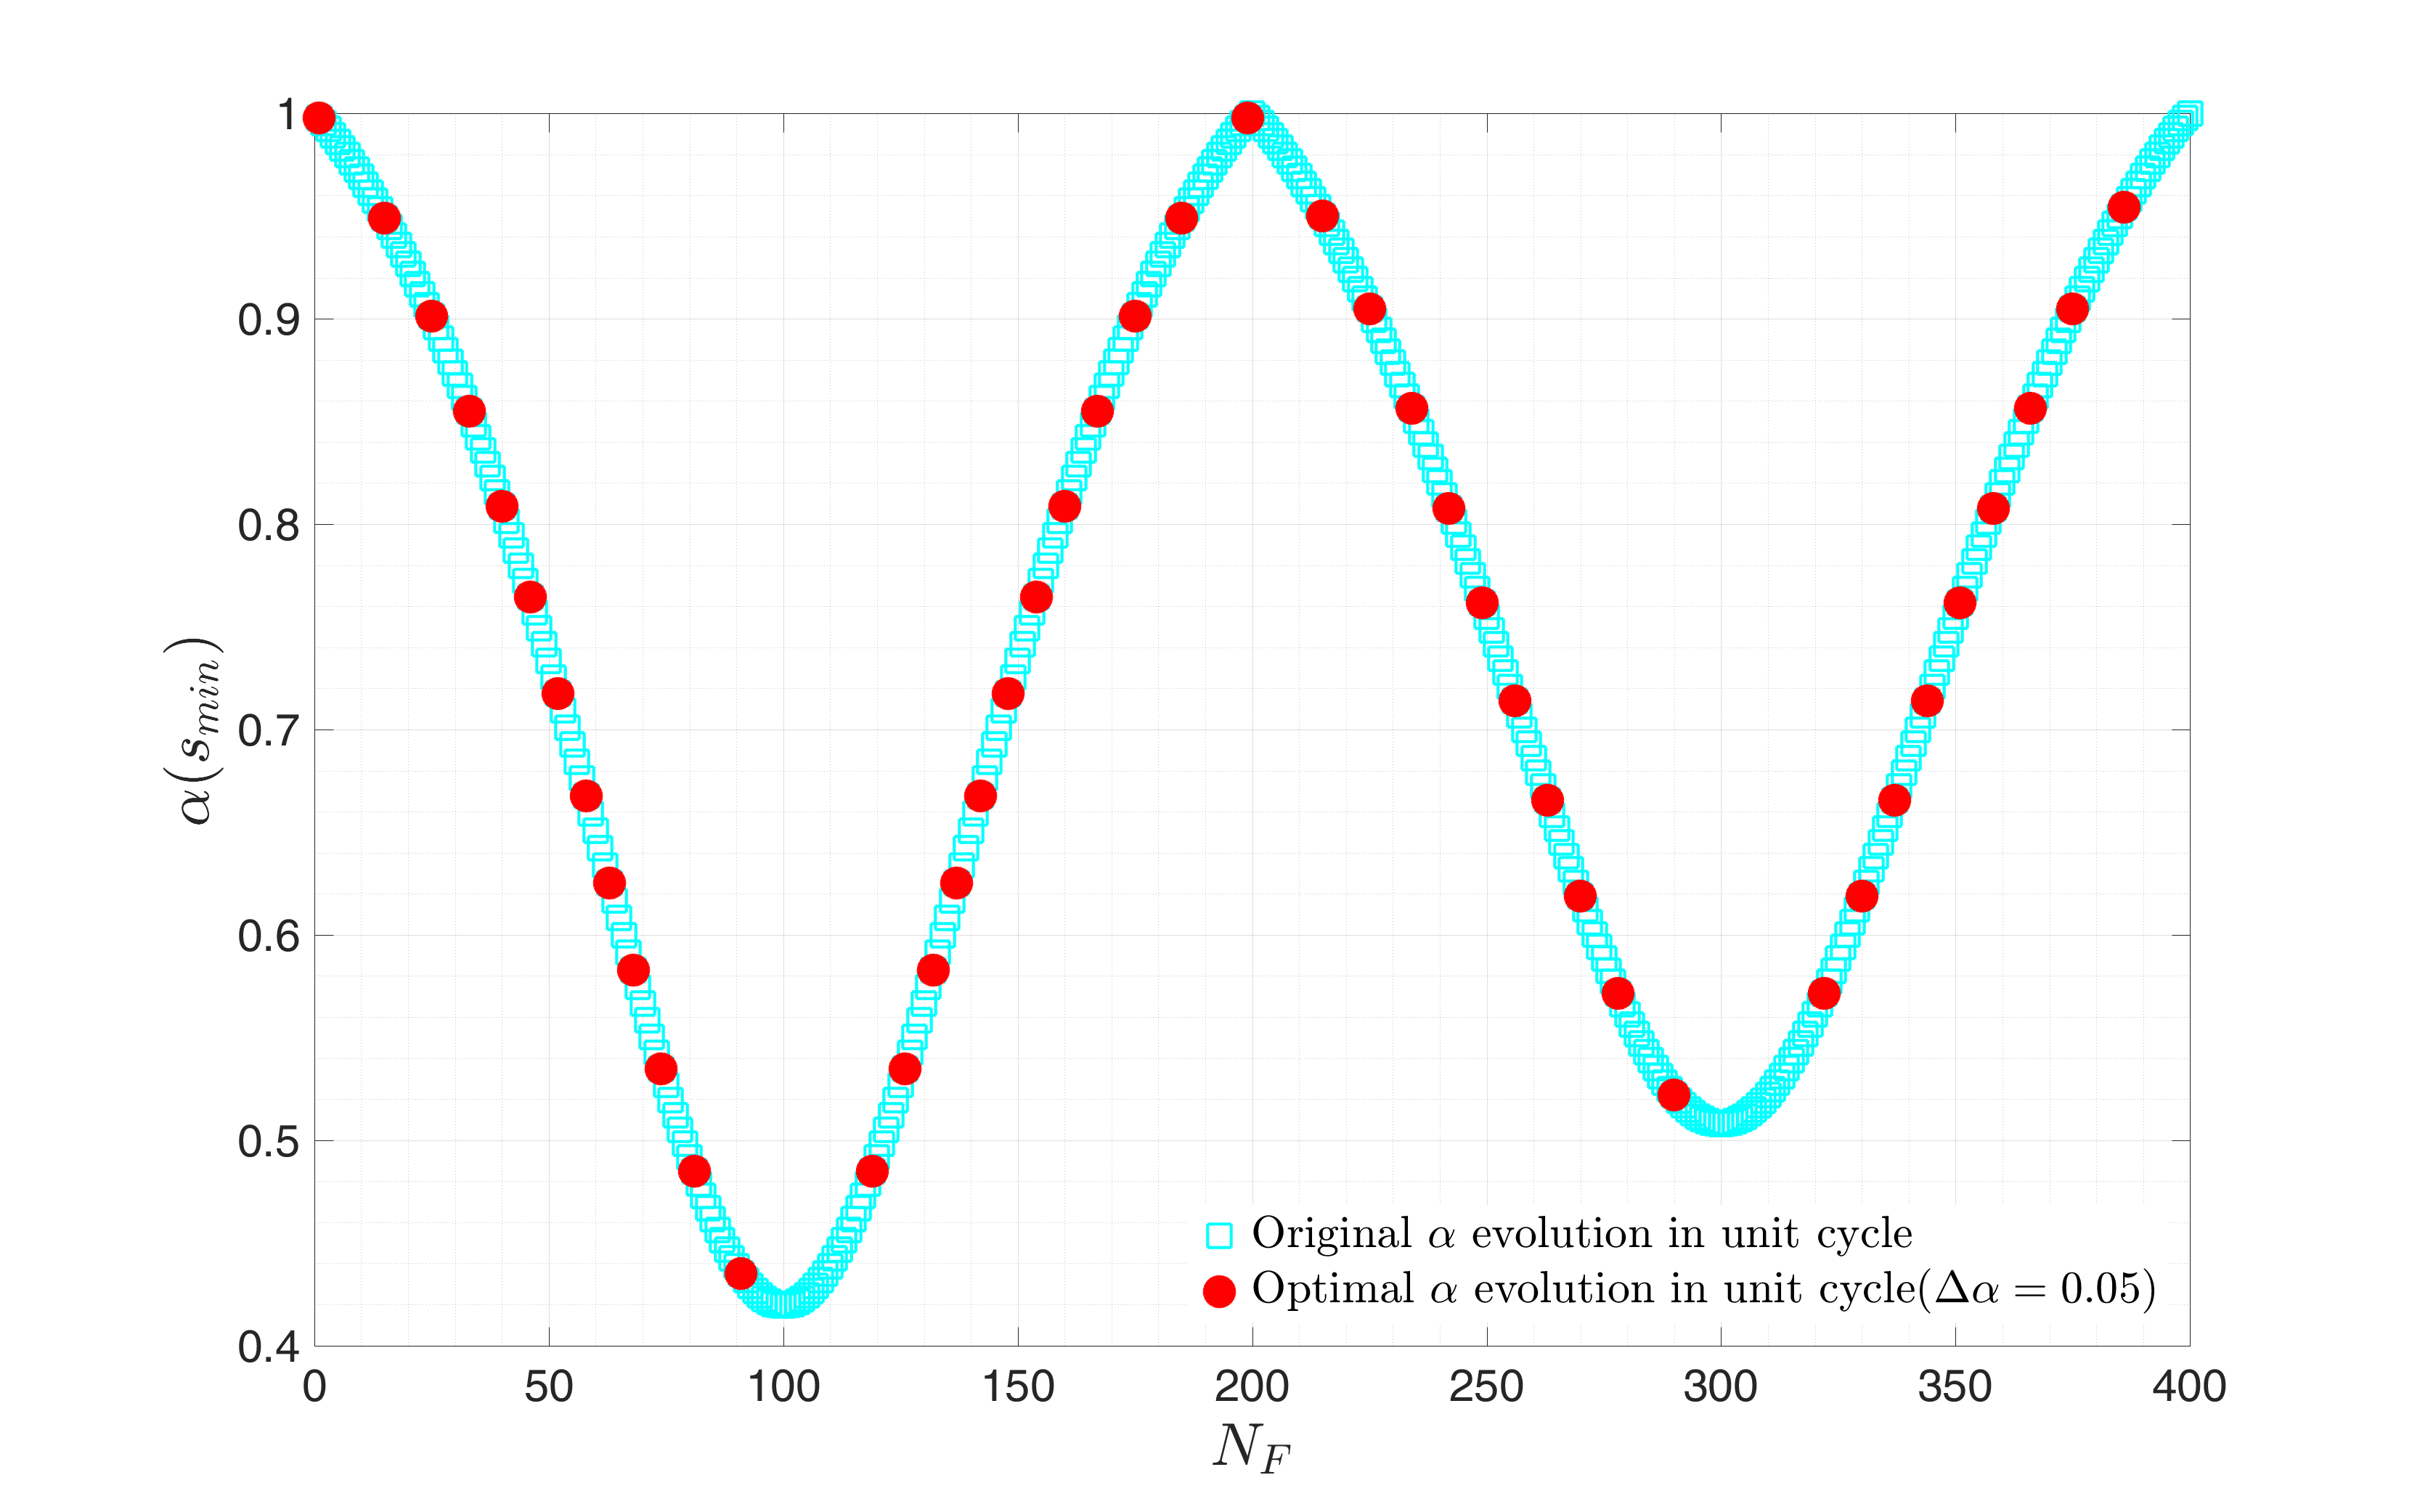
\includegraphics[width=0.8\textwidth]{figures//alpha_opt_vs_alpha_stepnumber.png} 
	\caption{Comparing numerical strategy with optimal time steps in one cycle with the old one, in this way the number of steps in unit cycle is reduced from 400 to 35, meaning a cost reduction factor of 0.0875 (with $\Delta\alpha=0.05$, $a=0.4$, $\lambda=0.1$, $\Sigma_y=230 MPa$, $\Sigma_{bending}=225 MPa$)}
	\label{fig.alpha_opt_vs_alpha_stepnumber}
\end{figure}

If $\alpha$ varies significantly, we use optimal time step numerical method to update $D$ during one time step. In more details, let us suppose that our first few cycles calculation with fine time steps $\Delta t$ has produced a sequence $\alpha(i)$ and $W_{cyc}(i)$ of exponent and dissipation at time $i\Delta t$. We then construct an adaptive time stepping strategy with variable time steps $\Delta t_{ref}(j)$, reference exponent $\alpha_{ref}(j)$ and dissipated energy $W_{ref}(j)$ by regrouping together adjacent time steps $\Delta t(i)$ with similar exponents $\alpha(i)$. This sequence is incremented as follows.


For $t_{ref}(j)$ and $\alpha_{ref}(j)=\alpha(t_{ref}(j))$ given, we set
$$\Delta t_{ref}(j)=\sum_{\substack{t(i)\geqslant t_{ref}(j)\\\left\| \alpha(i)-\alpha_{ref}(j)\right\|\leqslant \Delta\alpha }}\Delta t, \quad t_{ref}(j+1)=t_{ref}(j)+\Delta t_{ref}(j).$$
The same goes for the dissipated energy:
$$\Delta W_{ref}(j)=\sum_{\substack{t(i)\geqslant t_{ref}(j)\\\left\| \alpha(i)-\alpha_{ref}(j)\right\|\leqslant \Delta\alpha} }W_{cyc}(i) , \quad W_{ref}(j+1)=W_{ref}(j)+\Delta W_{ref}(j).$$

We finally use these new time steps with corresponding $\alpha_{ref}$ and $W_{ref}$ to update the damage by looping on all the following cycles with the new optimal time steps $j$ and cycles $N$, and updating damage in each cycle by:
\begin{equation}
D=D+D^{\alpha_{ref}(j)}\dfrac{\Delta W_{ref}(j)}{W_0},
\label{eq.optimal}
\end{equation}

with values $\alpha_{ref}(j)$ and $\Delta W_{ref}(j)$ precomputed in the first few cycles. This strategy is validated in \figref{fig.alpha_opt_vs_alpha_stepnumber}.

\vspace{6pt}
\textbf{Complexity analysis}
\vspace{6pt}

The optimal time step method clearly reduces the numerical cost. Typically, we assume the material has fatigue life of $1\times10^{6}$ cycles to failure and we implement $1000$ time steps in unit cycle. The reduction factor of points in unit cycle for example as in \figref{fig.alpha_opt_vs_alpha_stepnumber} equals $35/400=0.0875$. We can then compare the cost between full numerical strategy and the new one.

\begin{table}[!h]
\centering
\begin{tabular}{l|l}
\hline
Full numerical strategy: & $1000$ time steps $\times$ $64$ scales $\times$  $1\times10^{6}$ cycles       \\ \hline
Optimal cyclic strategy: & \begin{tabular}[l]{@{}l@{}} $1000$ time steps $\times$ $64$ scales $\times$  $5$ cycles until stabilization  \\$+$ $1\times10^{6}$ cycles $\times$ ($1000$ time steps $\times$ reduction factor)      \end{tabular}  \\ \hline
Ratio between optimal and full: & $\approx \dfrac{reduction \; factor}{64 \; scales}=\dfrac{1}{731}$       \\ \hline
\end{tabular}
\end{table}

The same strategy is applied to random loading situations which are made of repeated sequence of random loads:

\begin{itemize}
	\item calculation of dissipated energy and exponent on one sequence;
	
	\vspace{6pt}	
	
	\item time coarsening;
	
	\vspace{6pt}	
	
	\item repeated integration of damage through the different sequences using Eq.\ref{eq.optimal}.
		
	\vspace{6pt}
\end{itemize}
                          
In such a strategy, the extra cost of introducing multiple scales in the calculation becomes negligible as compared to the time integration of damage in the evolution process.

\begin{Figure}[]{S-N curve of bending test on 30NCD16 steel using numerical and analytical method (Eq.\eqref{eq.cycNF}) with different time steps. Data are those of table.\ref{tab:Sin}}[fig.sn-num-ana]
	\centerline{
		\graphfile*[38]{figures//SN_num_ana_stepnumber=30.png}[30 time steps in unit cycle($\beta=1.1$, $a=0.001$).]
		\graphfile*[38]{figures//SN_num_ana_stepnumber=100.png}[100 time steps in unit cycle($\beta=1.1$, $a=0.001$).]}
	\\
	\centerline{
		\graphfile*[38]{figures//SN_num_ana_stepnumber=30_err.png}[Relative error$\left( \dfrac{NF_{num}-NF_{analytical}}{NF_{analytical}}\right)$  with 30 time \protect \\ steps in unit cycle  ($\beta=1.1$, $a=0.001$)]
		\graphfile*[38]{figures//SN_num_ana_stepnumber=100_err.png}[Relative error$\left( \dfrac{NF_{num}-NF_{analytical}}{NF_{analytical}}\right)$   with 100 time \protect \\ steps in unit cycle  ($\beta=1.1$, $a=0.001$)]}
	\label{fig.sn-num-ana}
\end{Figure}

\newpage

Altogether, we have three numerical approaches for integrating damage.

\begin{enumerate}
	\item  Numerical results with varying $\alpha$(equally divide time in unit cycle), and do the scale integration all along the fatigue life time, which can be of high numerical cost$$\delta D=D^\alpha\frac{\dot{W}}{W_0}\delta t.$$
	This method only serves for qualification purposes.
	\vspace{6pt}
	
	\item  Numerical results with optimal time steps(equally divide $\alpha$in unit cycle), here we have $\Delta\alpha=0.01$, to reduce time steps needed, after several cycles adaptation we iterate using the recorded scalar values of $\alpha_{ref}$, $W_{ref}$ and $t_{ref}$ to decide fatigue life time.
	$$\delta D=D^{\alpha_{ref}}\frac{W_{ref}}{W_0}\delta t_{ref}.$$
	\vspace{6pt}
	
	\item  Analytical results after integration of D (with mean alpha from numerical strategy)$$N_F=\frac{W_0}{( 1-\alpha_m)W_{cyc}},$$ 
	which is derived from the differential equation
	$$\delta D=D^{\alpha_m}\frac{W_{cyc}}{W_0}\delta N.$$
\end{enumerate}	

Although method 2 is much more numerically efficient than the original numerical method 1, it is still not cheap in the experimental fitting process. We need the analytical formula method 3 to do the fitting process. To validate the feasibility, we now compare only the analytical(method 3) one and optimal time steps(method 2) one. The results are shown in \figref{fig.SNnumerical2methods} and \figref{fig.SNnumerical2methods2}, the relation ship between relative error and $\Delta \alpha$ with 2000 time steps in unit cycle is shown in  \figref{fig.errorNumAna0.02} and \figref{fig.errorNumAna0.01}.
\begin{figure}[!h]
	\centering
	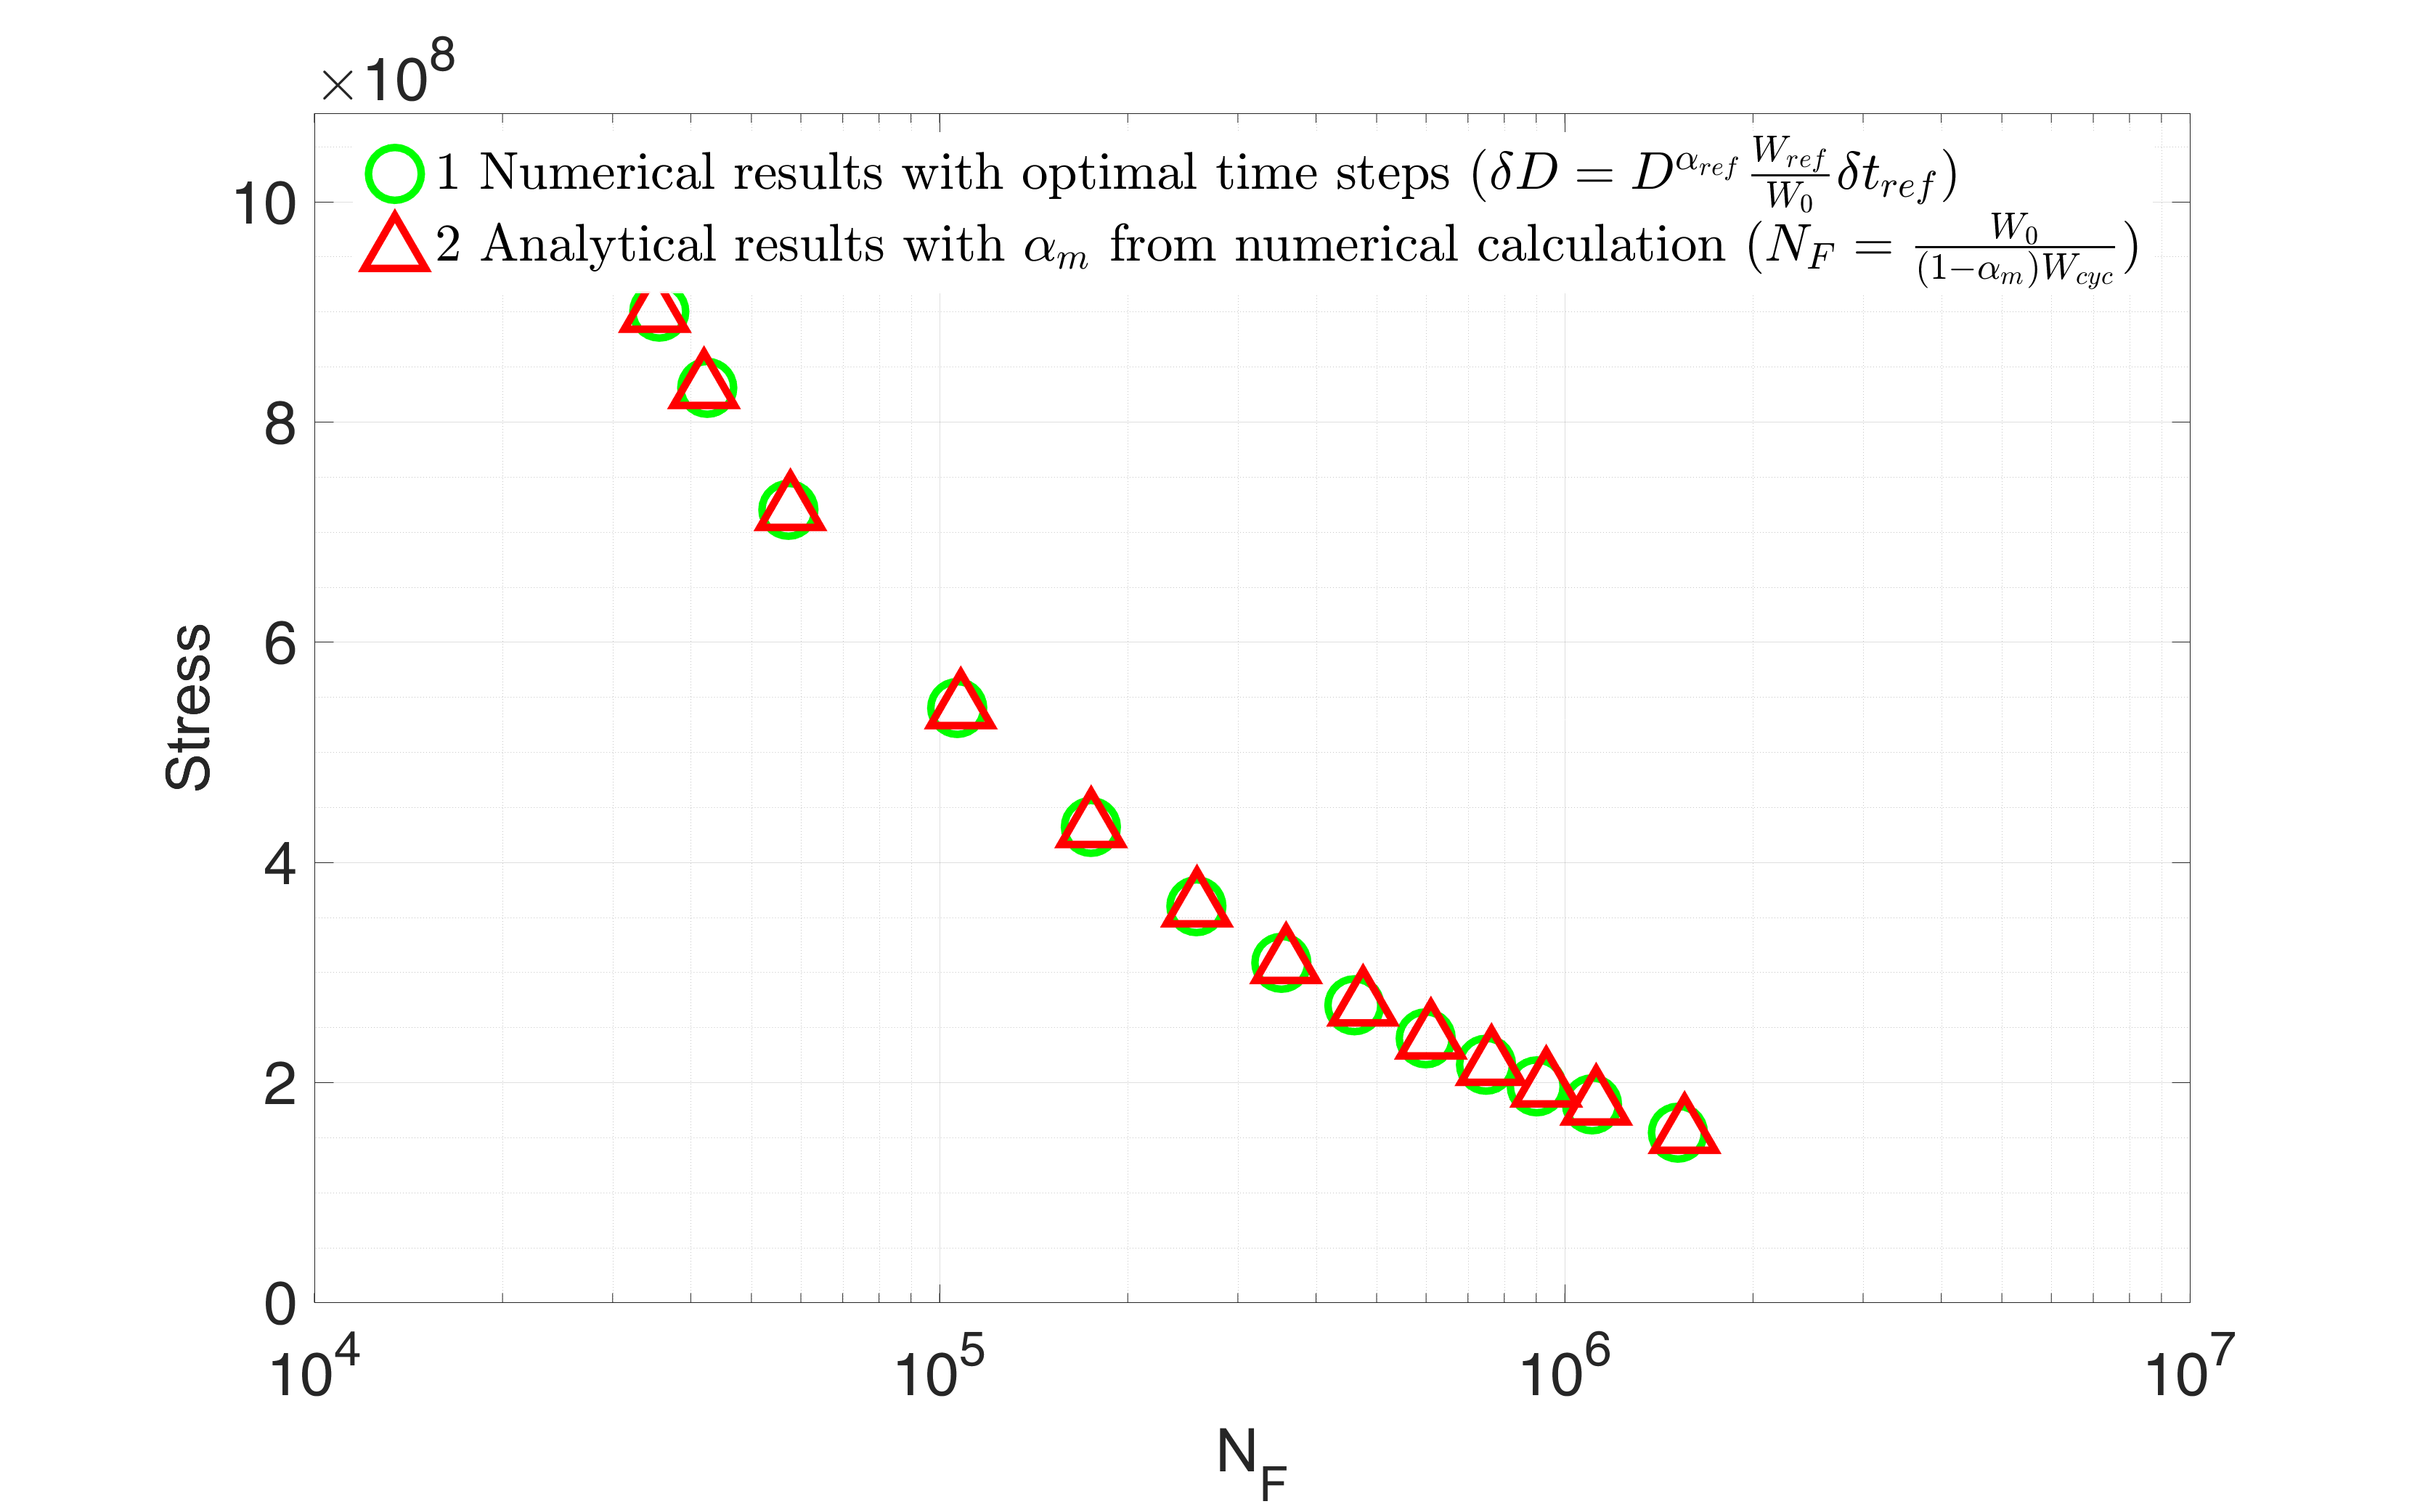
\includegraphics[width=\textwidth]{figures//SN_opt_ana_200_delta_alp=0.00002.png} 
	\caption{S-N curve using analytical and numerical results with optimal time steps methods ($\beta=1.1$, $a=0.01$, $\Delta \alpha=2E-5$ in unit cycle), yielding 200 full time steps reduced to 197 optimal time steps}
	\label{fig.SNnumerical2methods}
\end{figure}
\begin{figure}[!h]
	\centering
	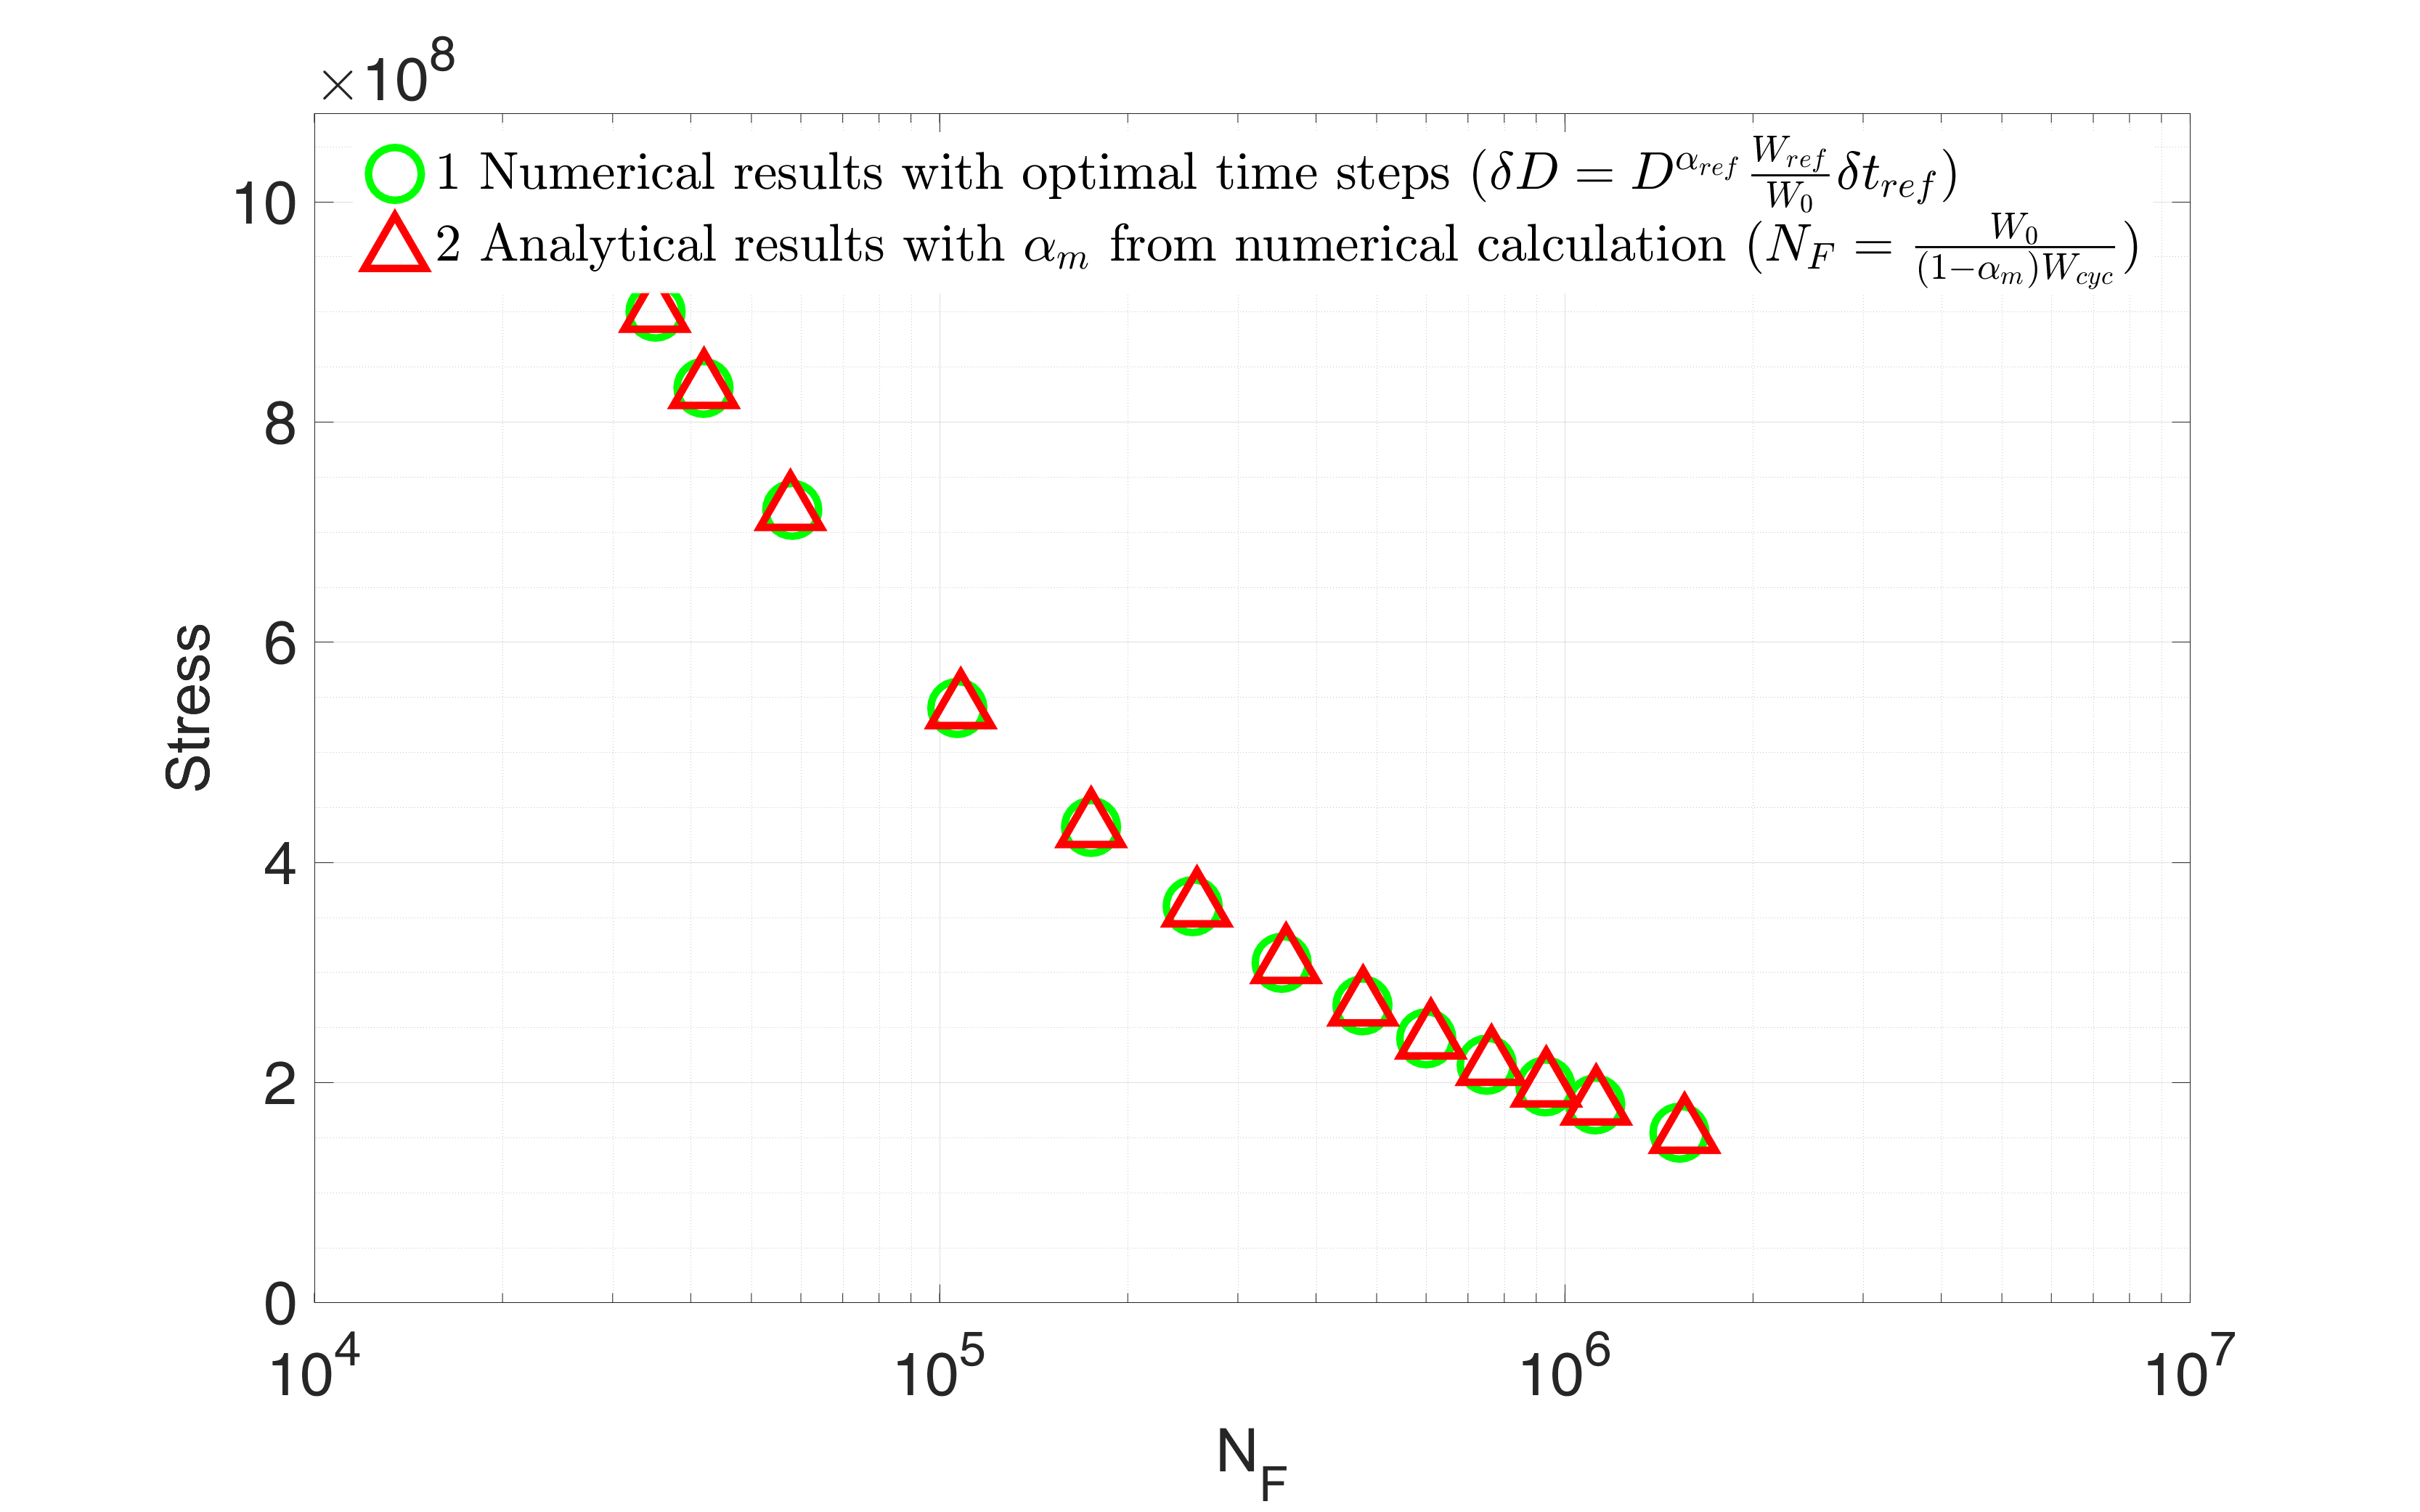
\includegraphics[width=\textwidth]{figures//SN_opt_ana_200_delta_alp=0.00001.png} 
	\caption{S-N curve using analytical and numerical results with optimal time steps methods ($\beta=1.1$, $a=0.01$, $\Delta \alpha=1E-5$ in unit cycle), yielding 200 full time steps reduced to 199 optimal time steps}
	\label{fig.SNnumerical2methods2}
\end{figure}
\begin{figure}[!h]
	\centering
	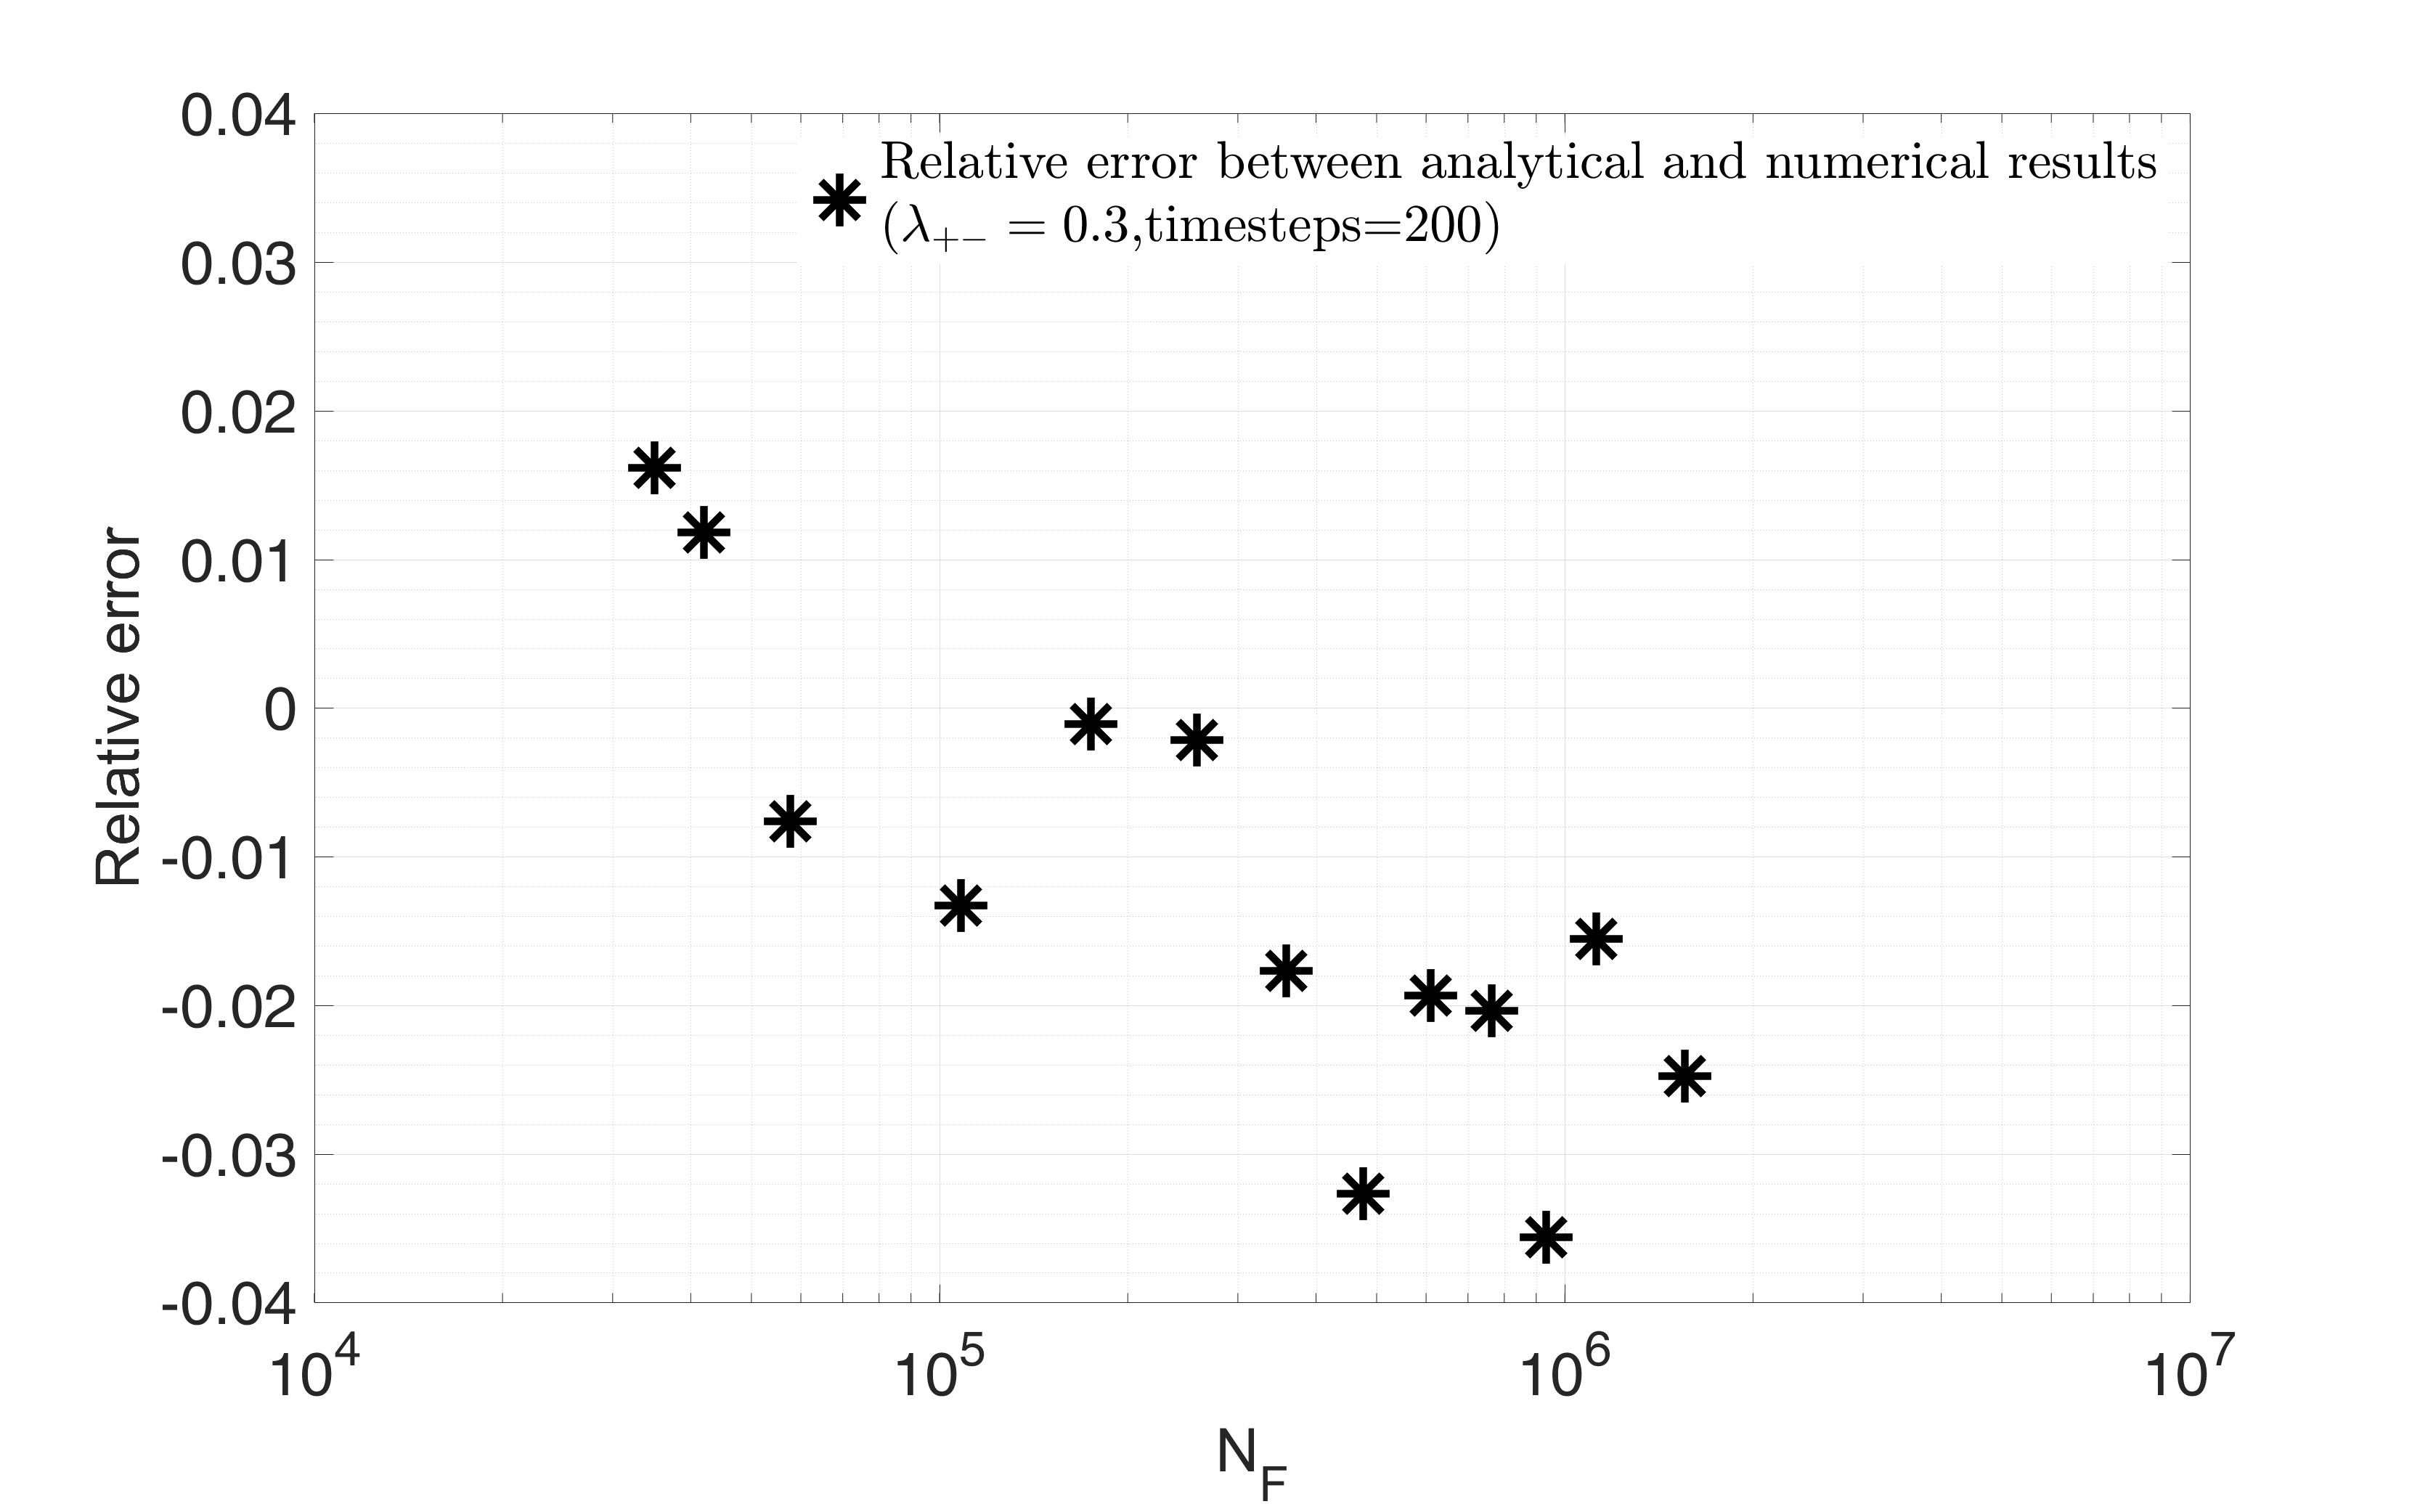
\includegraphics[width=\textwidth]{figures//SN_opt_ana_200_delta_alp=0.00002_err.png} 
	\caption{Relative error $\left( \dfrac{NF_{opt}-NF_{analytical}}{NF_{analytical}}\right)$  between analytical and numerical results with optimal time steps methods ($\beta=1.1$, $a=0.01$, $\Delta \alpha=2\times10^{-5}$ in unit cycle)}	
	\label{fig.errorNumAna0.02}
\end{figure}
\begin{figure}[!h]
	\centering
	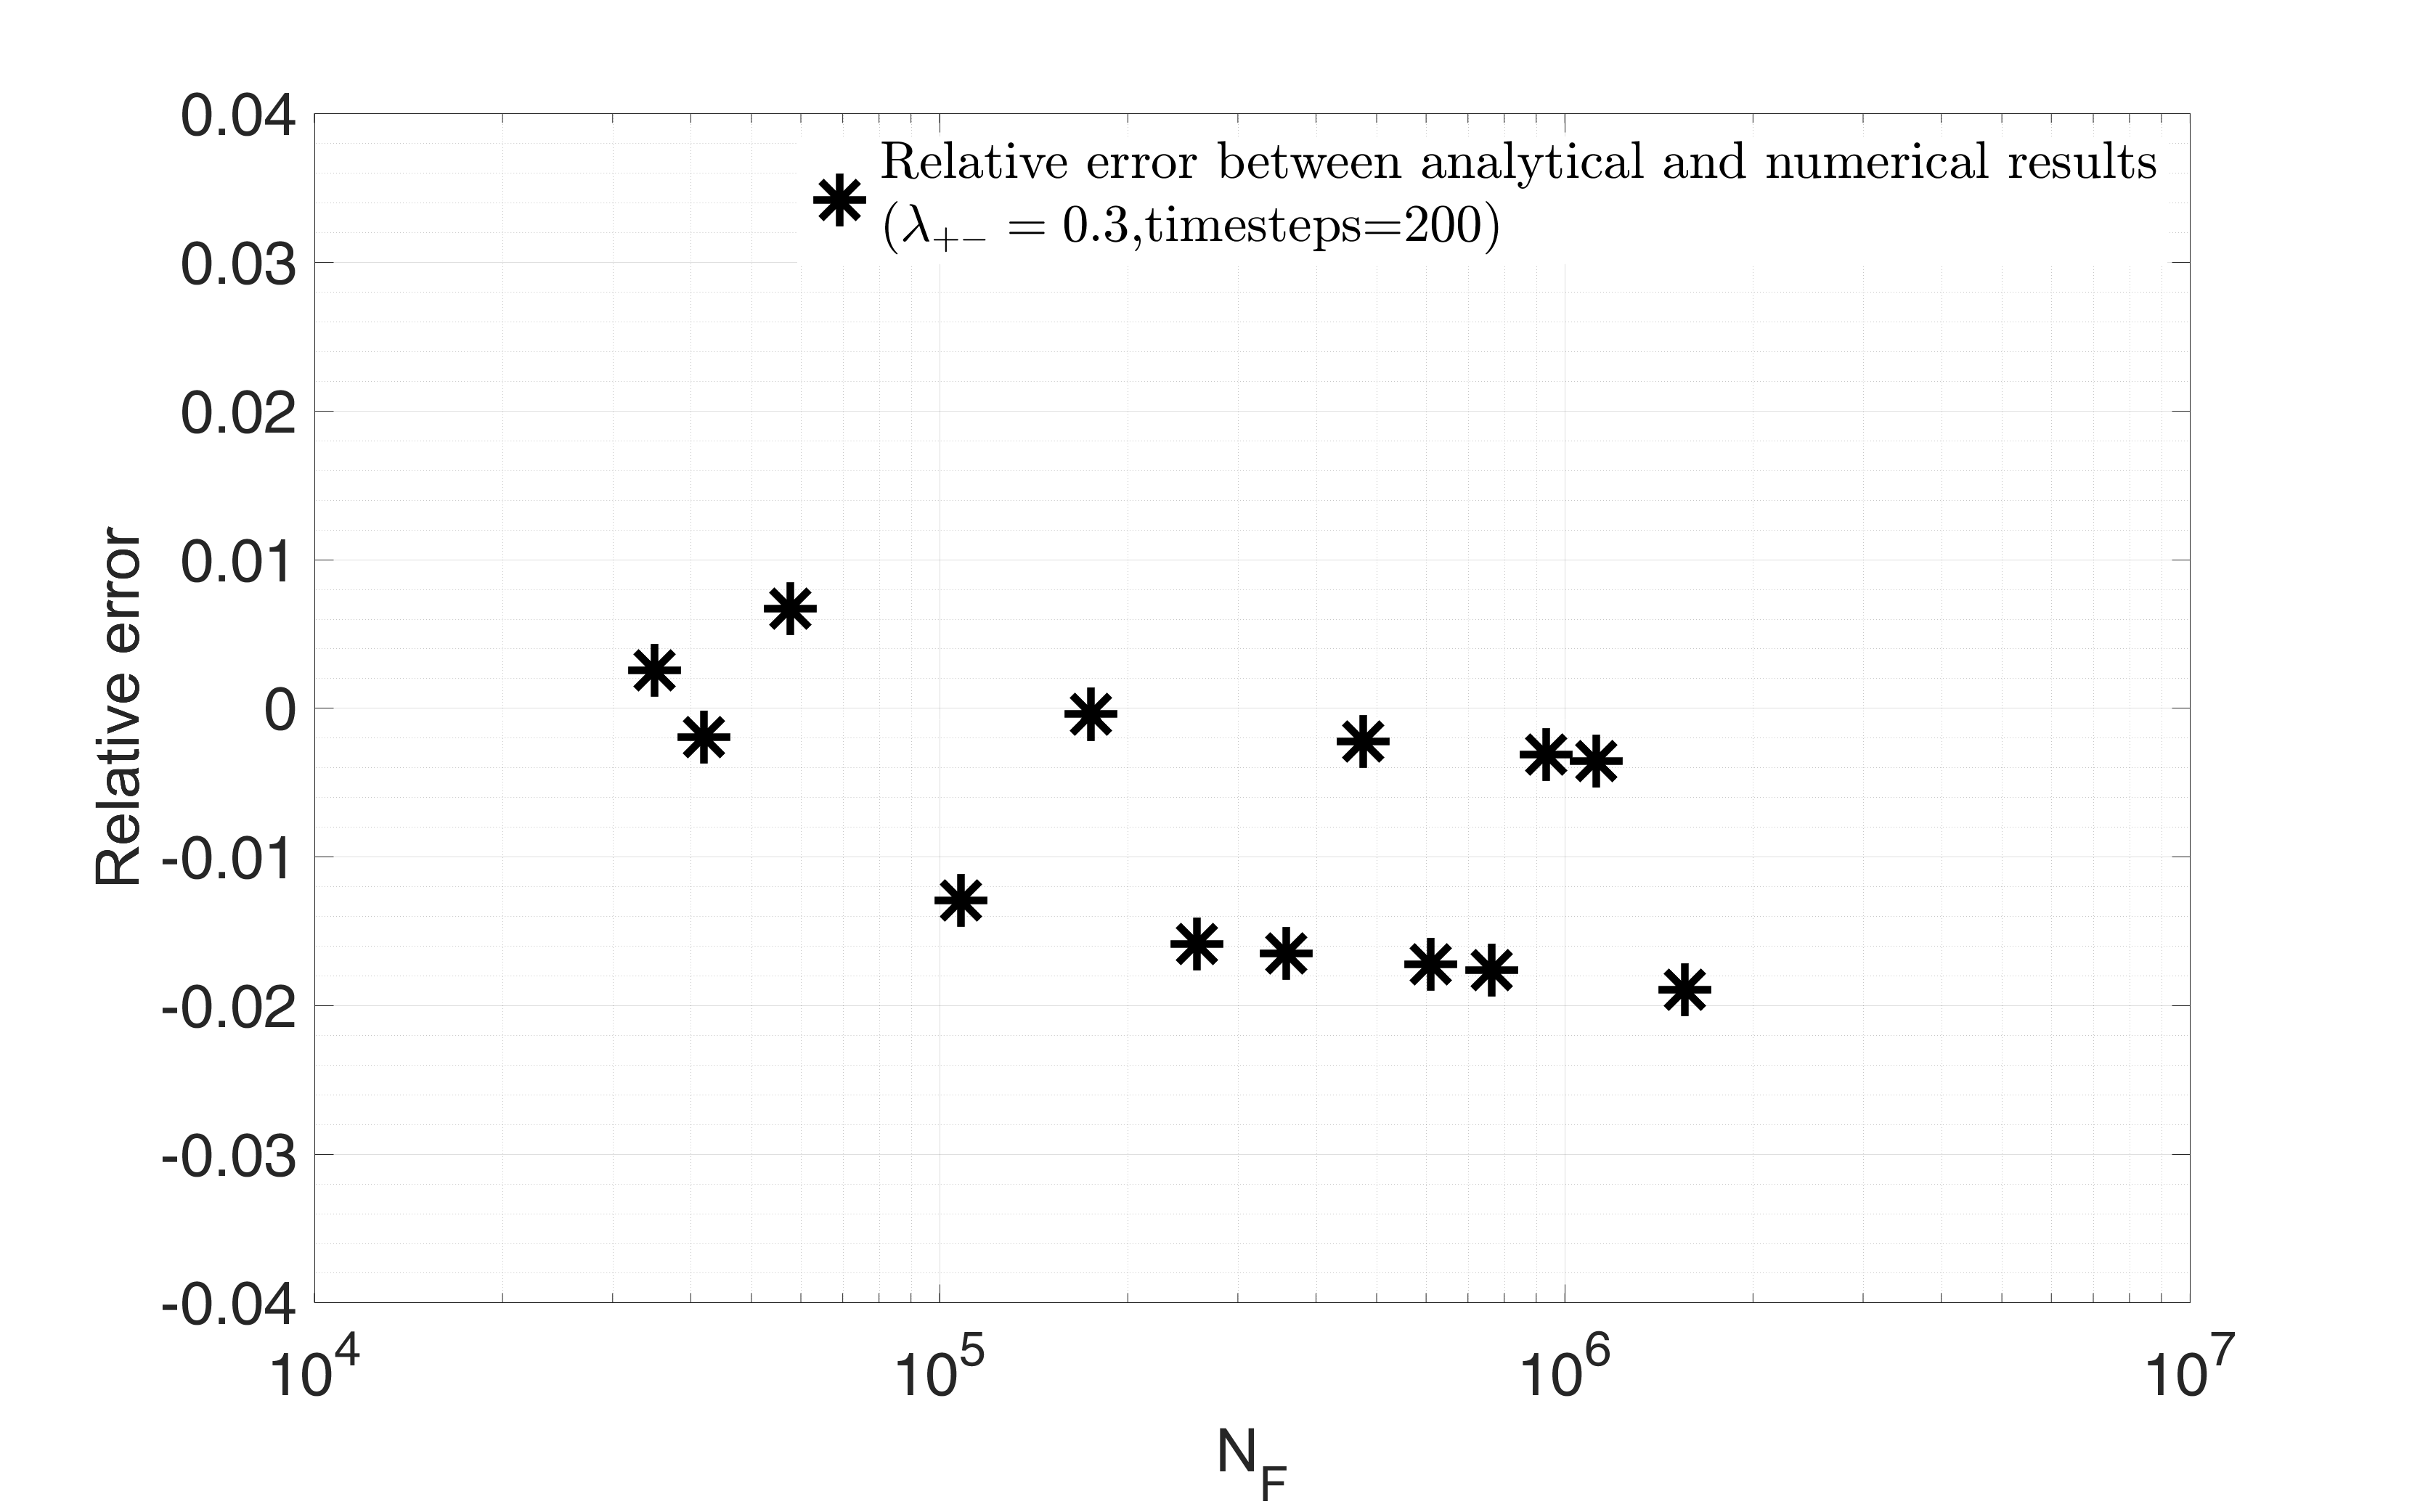
\includegraphics[width=\textwidth]{figures//SN_opt_ana_200_delta_alp=0.00001_err.png} 
	\caption{Relative error $\left(\dfrac{NF_{opt}-NF_{analytical}}{NF_{analytical}}\right)$  between analytical and numerical results with optimal time steps methods ($\beta=1.1$, $a=0.01$, $\Delta \alpha=1\times10^{-5}$ in unit cycle)}
	\label{fig.errorNumAna0.01}
\end{figure}

Now we can conclude that with more time steps in unit cycle, we get closer results with the original numerical method(method 2) in HCF regime. With smaller $\Delta \alpha$ value, we get less relative error between numerical(method 3) and analytical(method 1) results. This indicates that in constant amplitude cyclic loading, with moderate values of $\beta$ it is feasible to use the analytical formula, given $\alpha_m$ is calculated using sufficient large time steps and small $\Delta \alpha$ in the first several cycles.

\clearpage
\section{Validation on recovery tests}
\label{sec:5.8}
\subsection{Recovery of Chaboche law on cyclic loading}
The test is first performed on a sinusoidal uniaxial load $\Sigma_{11}(t)=Asin(t)$, giving a deviatoric amplitude$S_{a}(t)=\sqrt{J_{2,a}(dev\uuline{\Sigma(t)})}$  so that $S_{a}(t)=\left\| \sqrt{\dfrac{1}{3}}\Sigma_{11}(t)\right\| $. We use parameters in Table.\ref{tab:Sin} to recover the classic Chaboche law in cyclic loading.
\begin{table}[!h]
\centering
\begin{tabular}{ll}
\hline
\textbf{Parameters}                                         & \textbf{Value}                    \\ \hline
Young's modulus                                             & $E=191$ GPa                       \\
Hardening parameter                                         &  $k=1$ GPa \\
Weakening scales distribution exponent                      & $\beta=1.5$                             \\
Hydrostatic pressure sensitivity                            & $\lambda_{+-}=0.6$                     \\
Macroscopic yield stress                                    & $\sigma_y=1080$ MPa              \\
Sequencing effect sensitivity                               & $a=0.1$                        \\
Dissipated energy to failure per unit volume                & $W_0=5$ MJ(MPa)                       \\ \hline
\end{tabular}
\caption{Material parameters in a simple cyclic load }
\label{tab:Sin}
\end{table}

We use matlab to numerically realize our method. The plot of $\left\|  \uline{\uline{S}}-\uline{\uline{b}}\right\|_{trial}$ and $\left\|  \uline{\uline{S}}-\uline{\uline{b}}\right\|$ during the first cycles at two different scales($s_{3}=1.21$ and $s_{10}=1.13$) are shown in \figref{fig.trialsin0} and \figref{fig.trialsinm}. We use here a fixed value of $\lambda$($\lambda_+=\lambda_-$), thus the local yield limit is reduced in traction and increased
in compression.

\begin{figure}[!h]
\centering
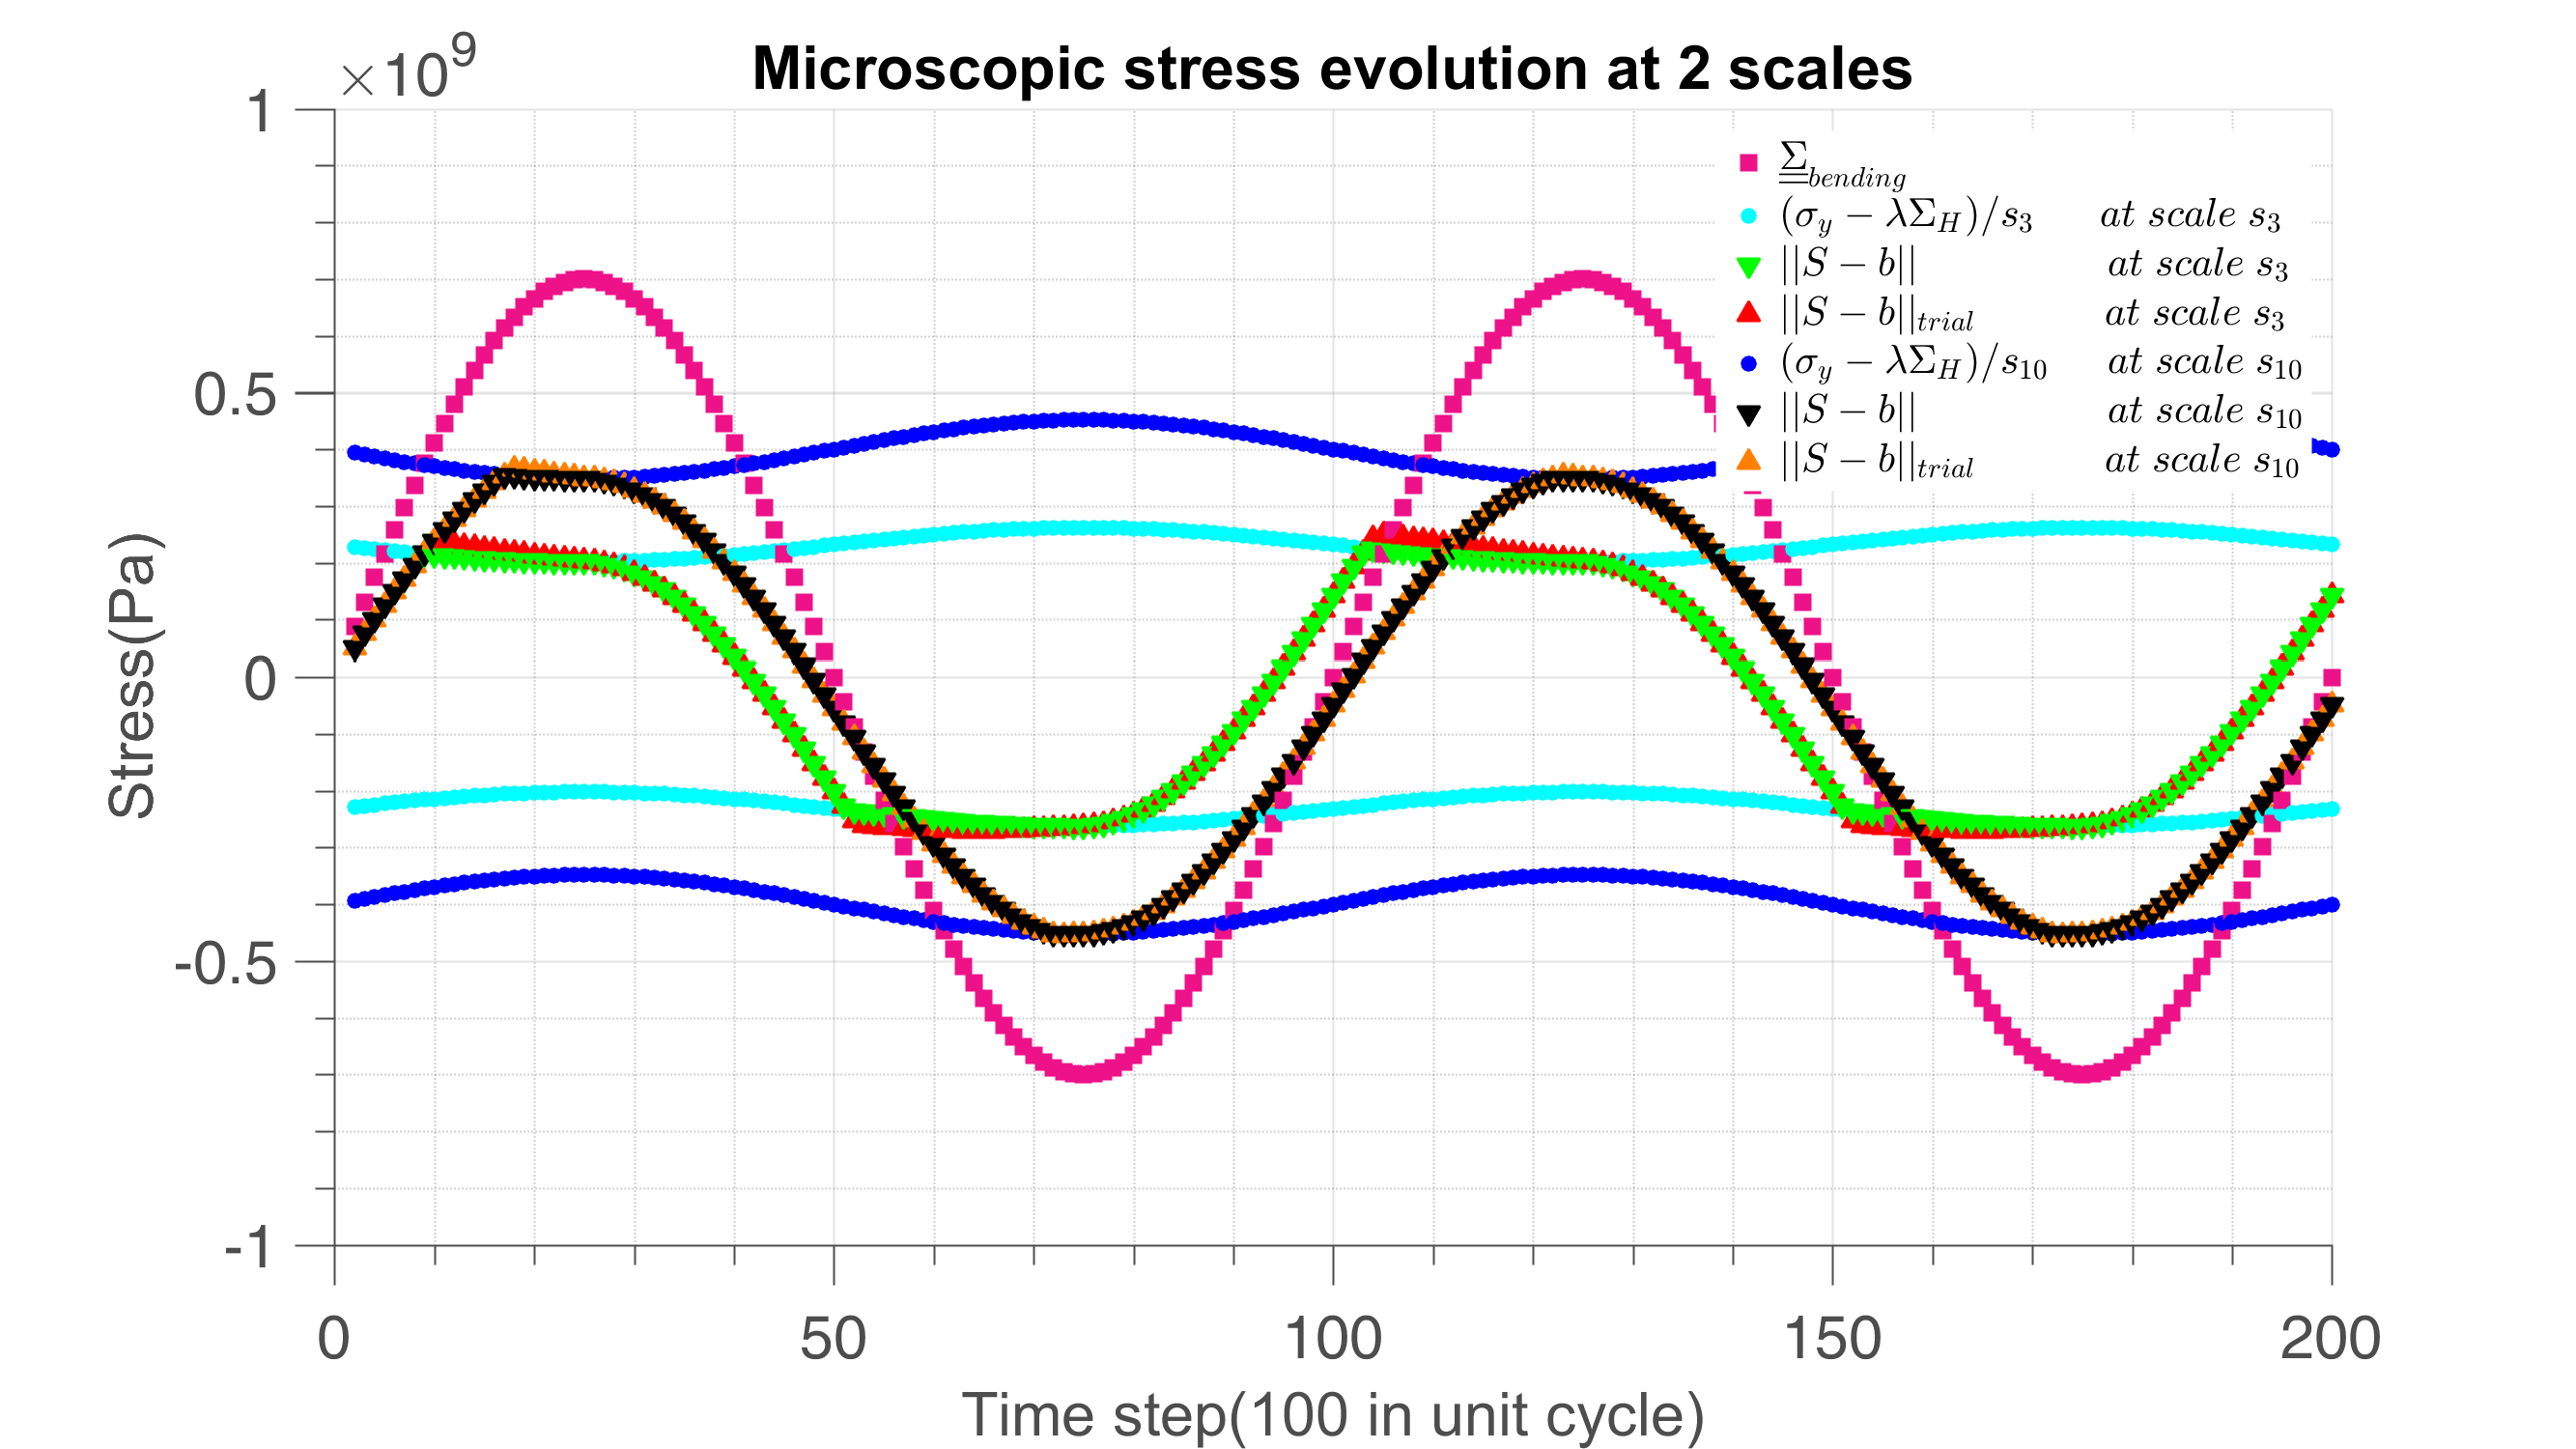
\includegraphics[width=\textwidth]{figures//trialsin_0.png} 
\caption{Microscopic $\left(  \uline{\uline{S}}-\uline{\uline{b}}\right)_{trial}$ and $\left( \uline{\uline{S}}-\uline{\uline{b}}\right)$ evolution with time under different weakening scales($s_{3}=1.21$ and $s_{10}=1.13$) in sinusoidal load with zero mean stress}
\label{fig.trialsin0}
\end{figure}
\begin{figure}[!h]
\centering
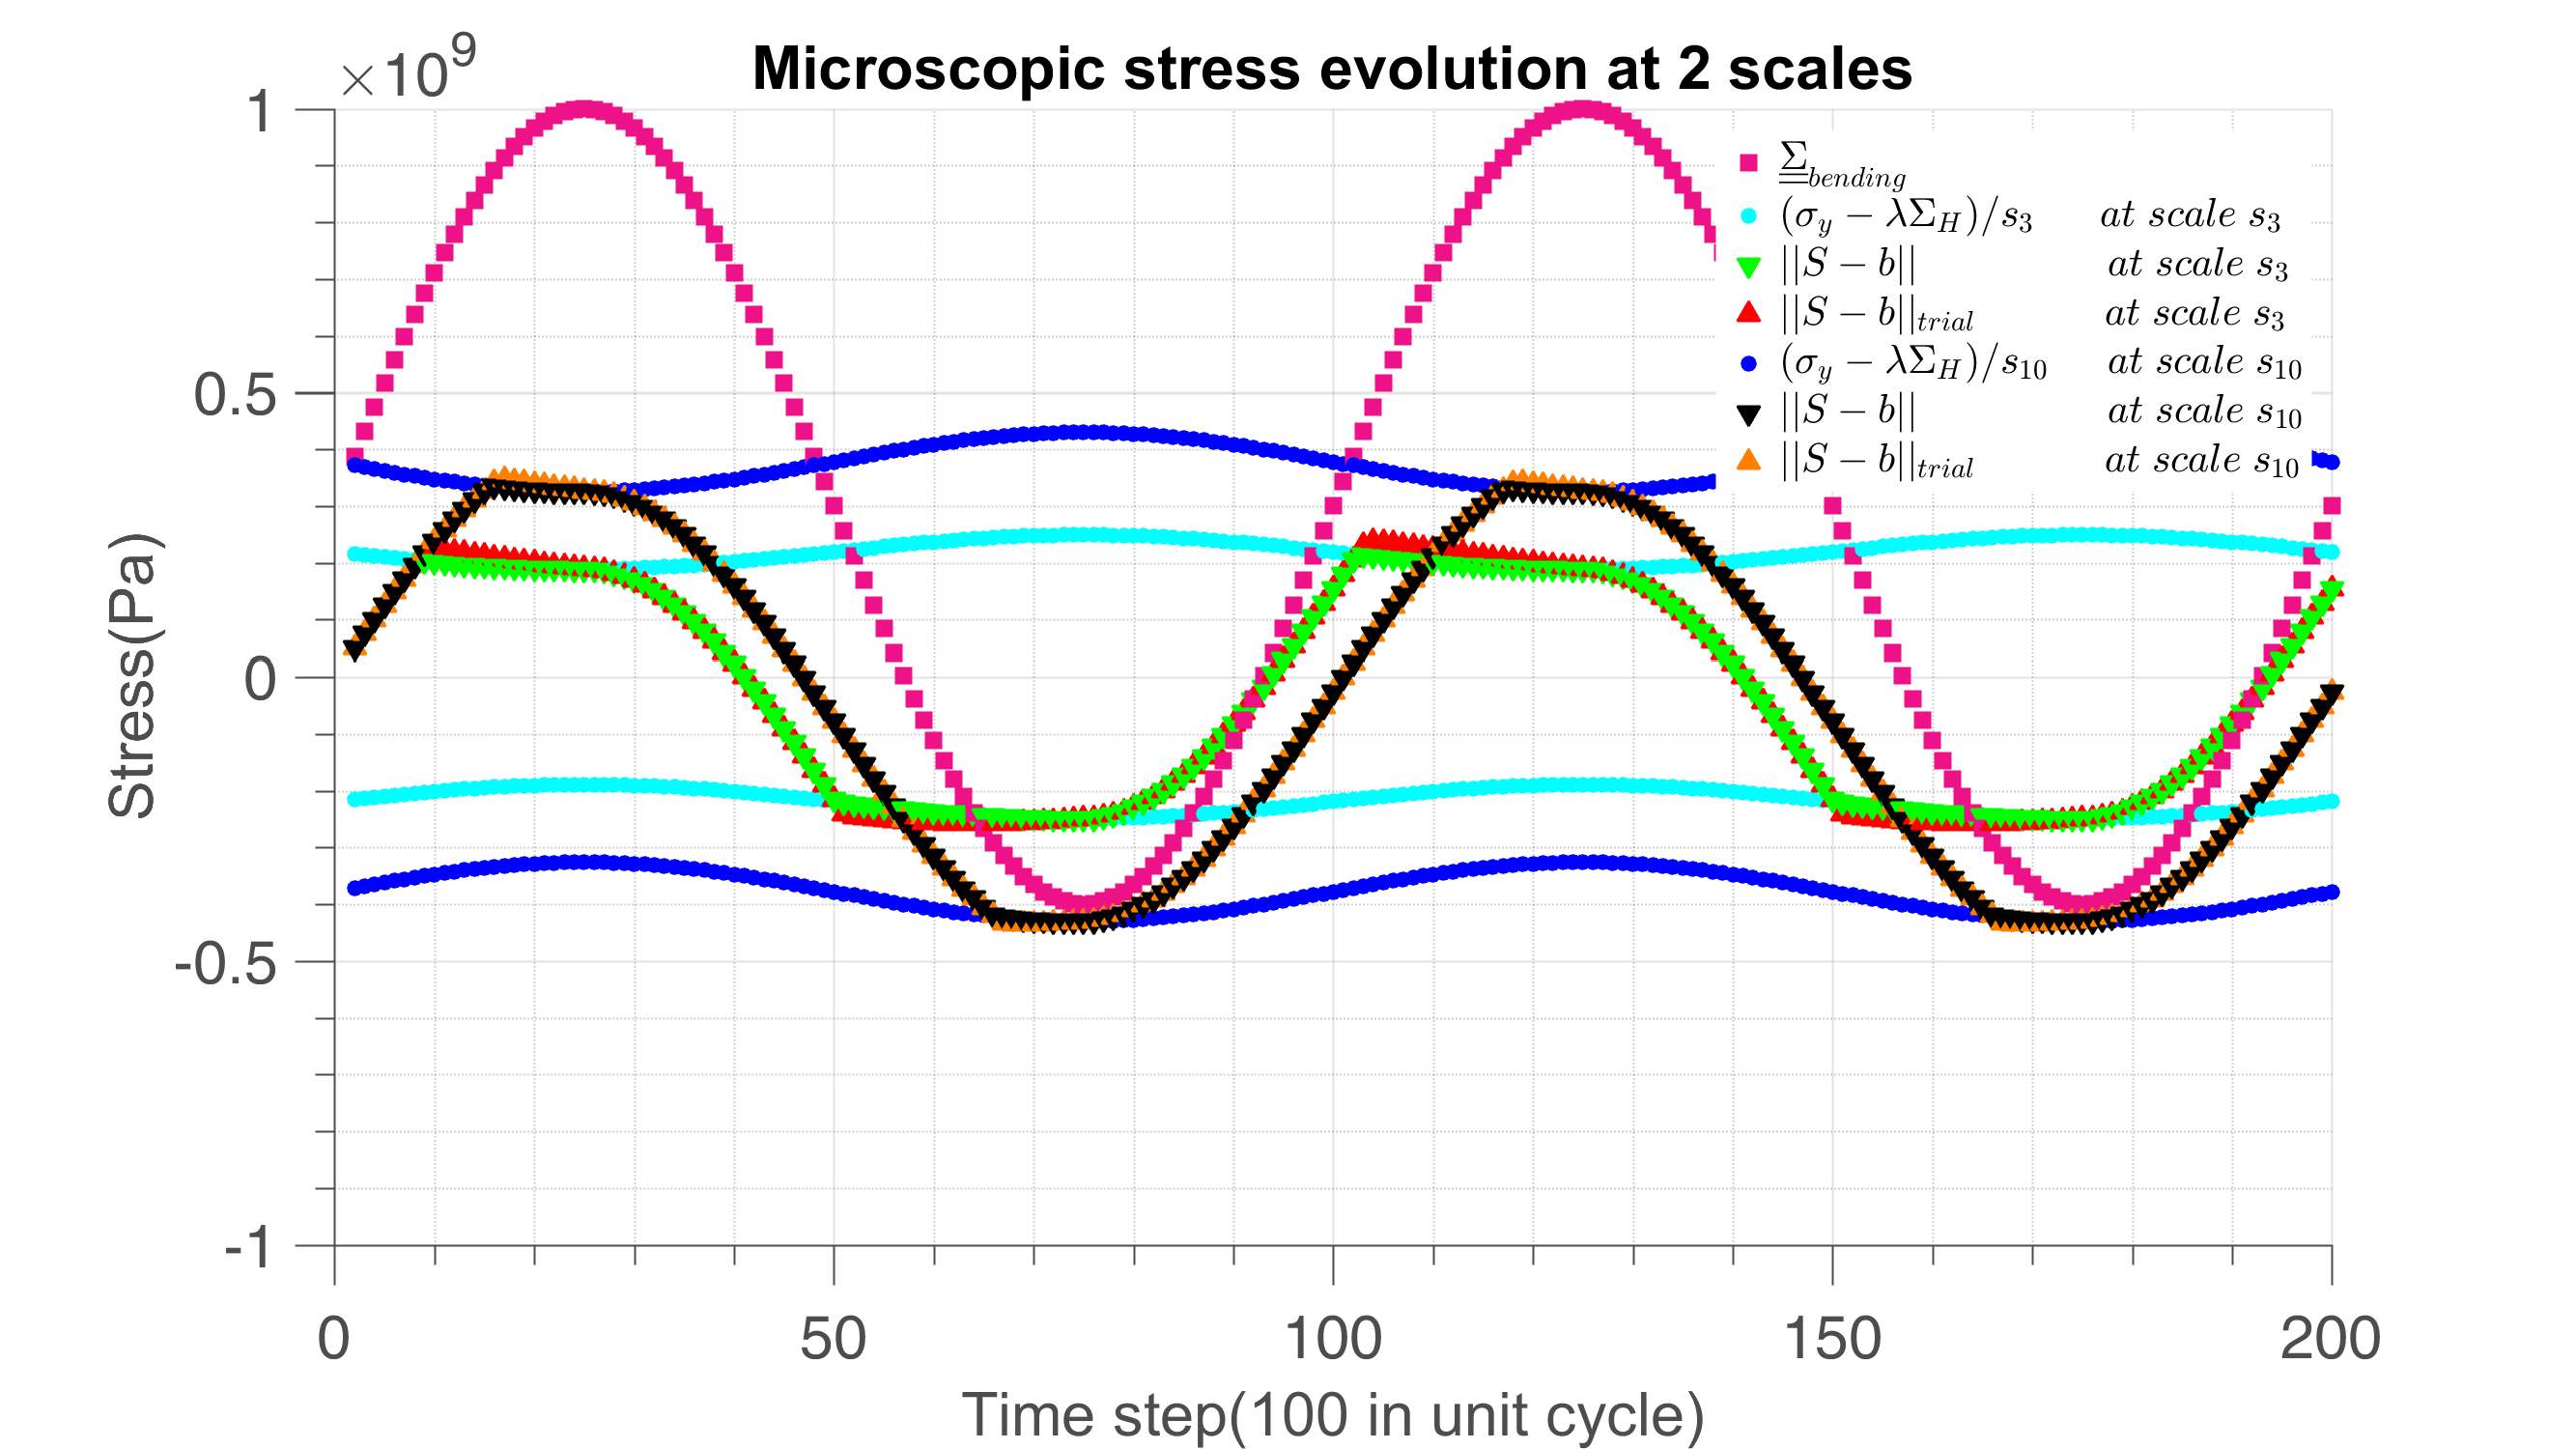
\includegraphics[width=\textwidth]{figures//trialsin_m.png} 
\caption{Microscopic $\left(  \uline{\uline{S}}-\uline{\uline{b}}\right)_{trial}$ and $\left( \uline{\uline{S}}-\uline{\uline{b}}\right)$ evolution with time under different weakening scales($s_{3}=1.21$ and $s_{10}=1.13$) in sinusoidal load with mean stress=300 MPa}
\label{fig.trialsinm}
\end{figure}

The time history of dissipated energy is depicted in \figref{fig.W3methods}. We scale $S_{a}$ in the plot to see more clearly the relation between energy dissipation and stress intensity. The choice of $\alpha$ does not affect $W$; it only concerns damage accumulation rate. Smaller $\alpha$ causes faster accumulation.

The ``jump'' in energy evolution is due to activation of new scales while in-between two scales the dissipated energy follows the stress increment at each time step. In other words, because in our method the dissipated energy $W$(\figref{fig.W3methods}), sums energy dissipation at all scales, any additional violation of $\left\|S-b \right\|_{trial}$ at local yield limit(\figref{fig.trialsin0}) introduces an additional dissipation. 

\begin{figure}[!h]
\centering
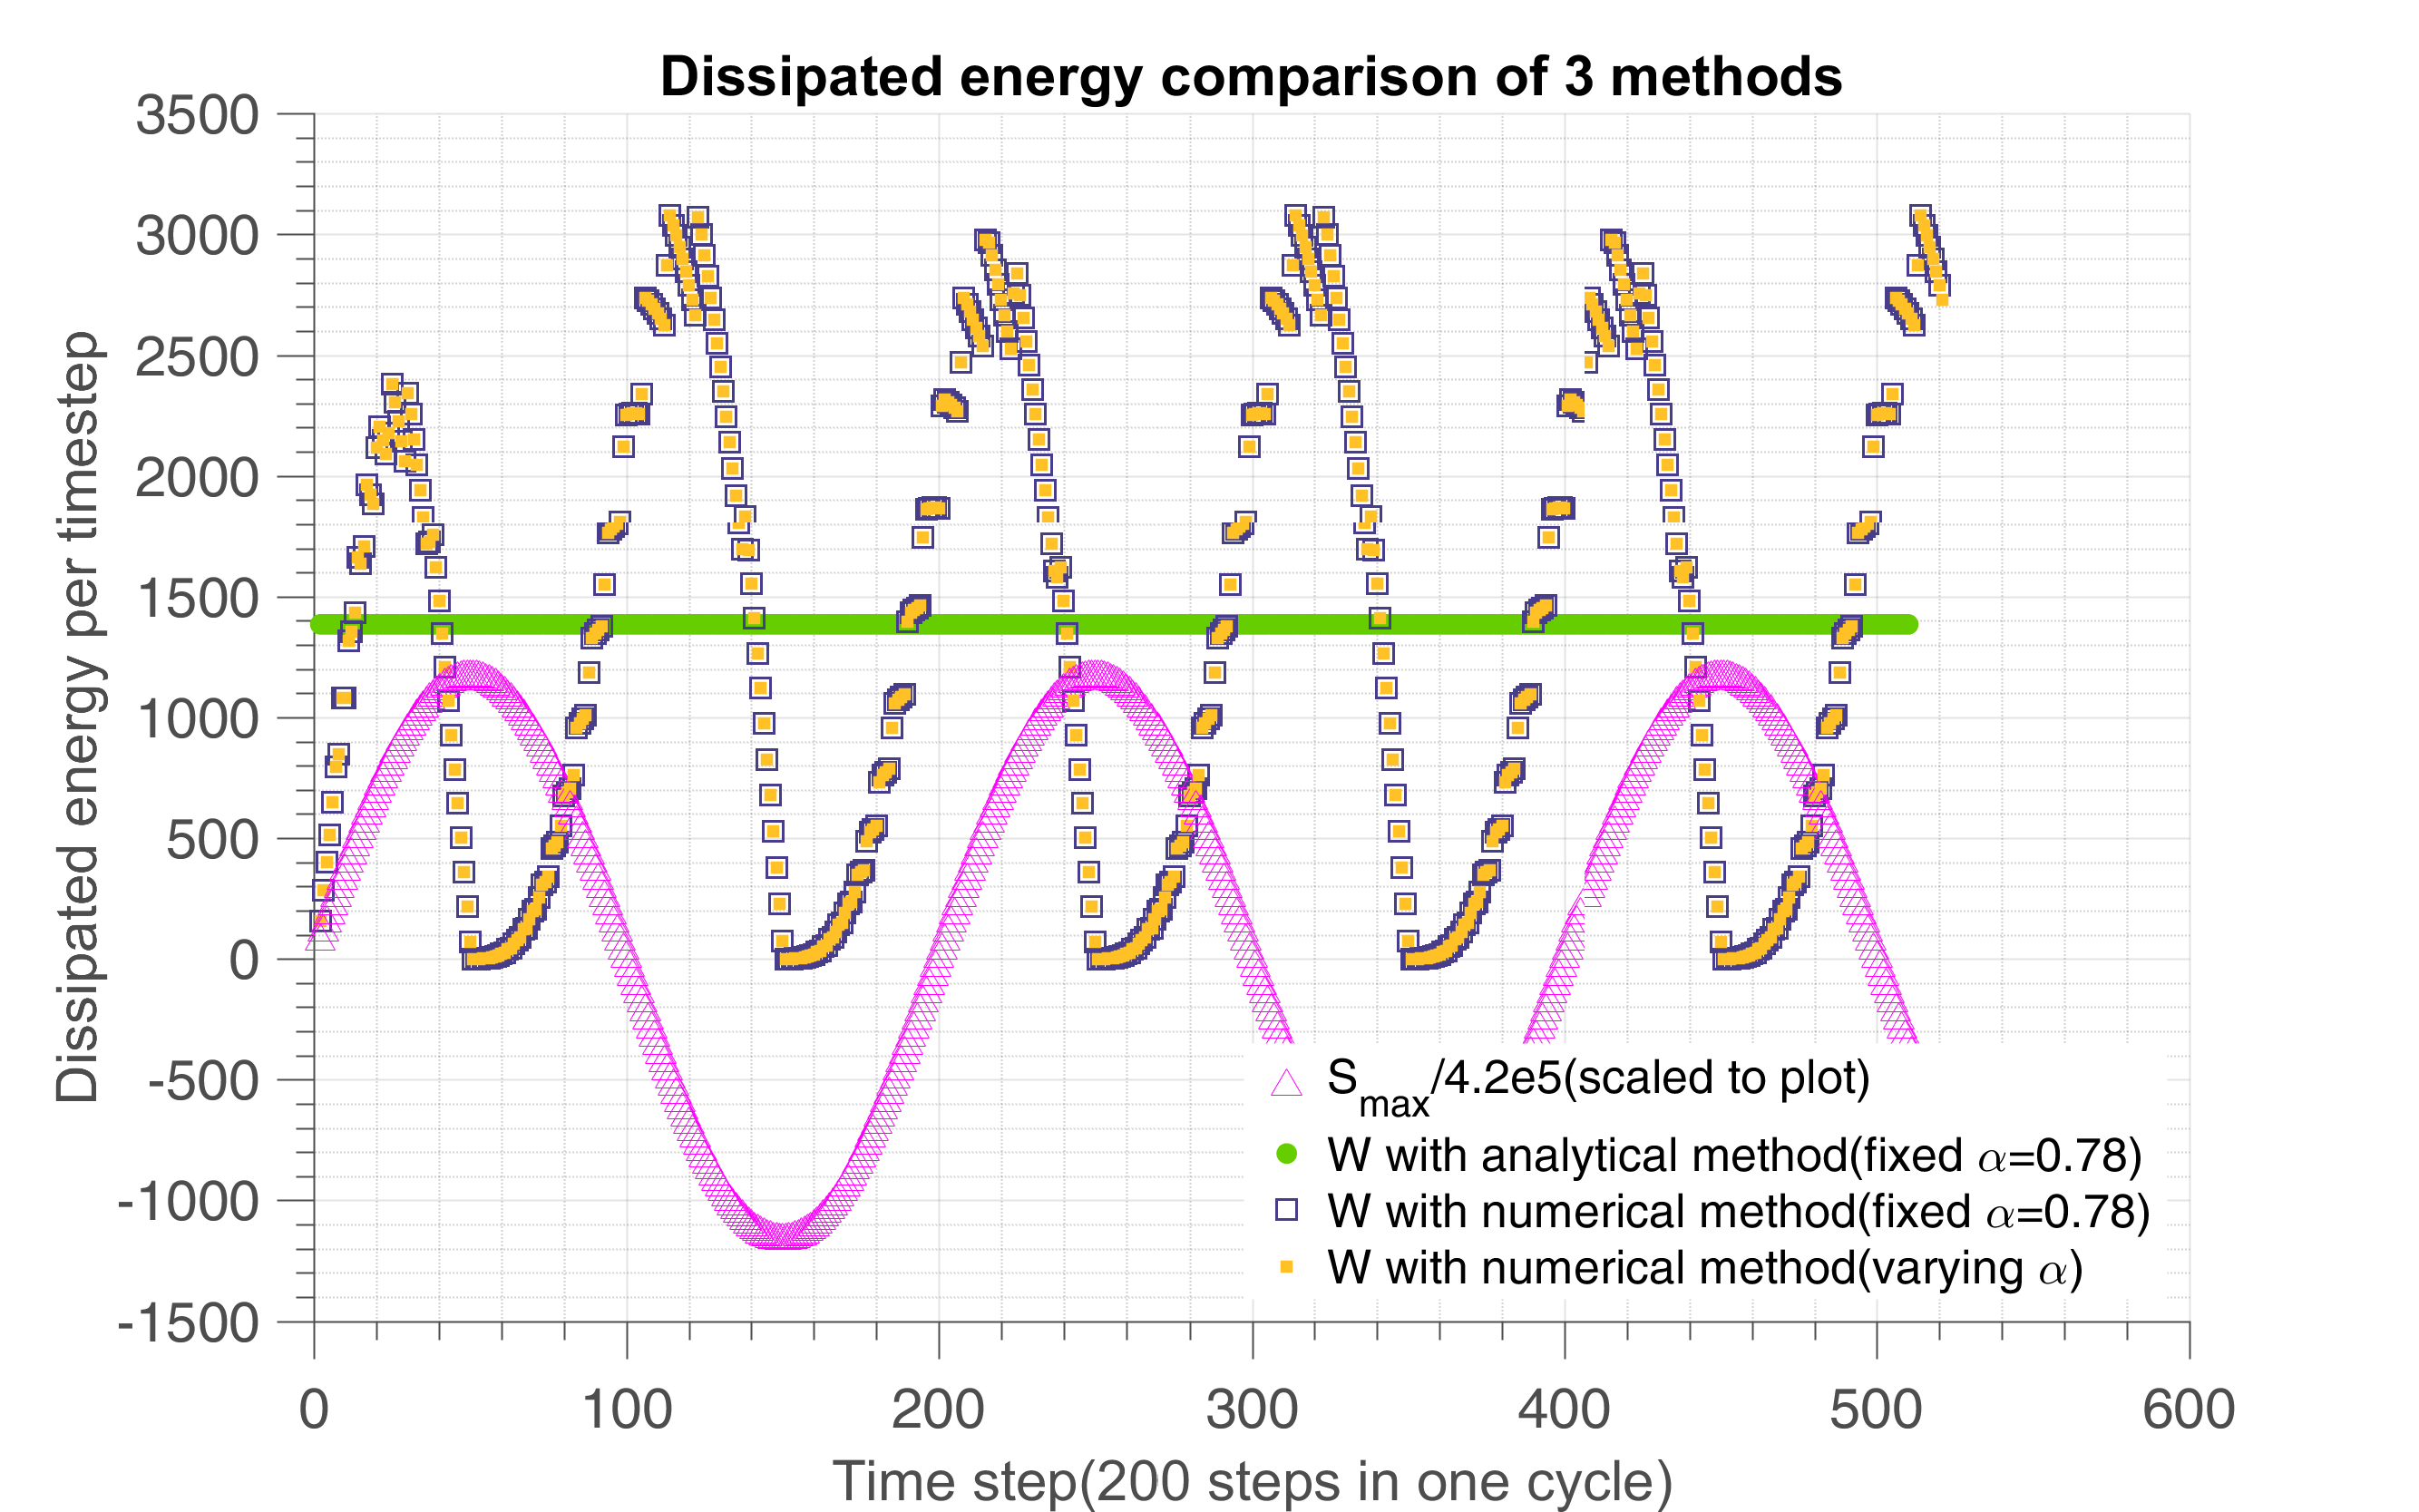
\includegraphics[width=0.95\textwidth]{figures//W_3methods.png} 
\caption{Validation of dissipated energy in all scales with analytical(method 3) and numerical method(method 1) with $\beta=1.1$,$\Sigma=0.85\sigma_y$. The time evolution of $\alpha$ does not play a role in the dissipation calculation which is normal since $\alpha$ does not enter in the dissipation calculation }
\label{fig.W3methods}
\end{figure}
\begin{figure}[!h]
	\centering
	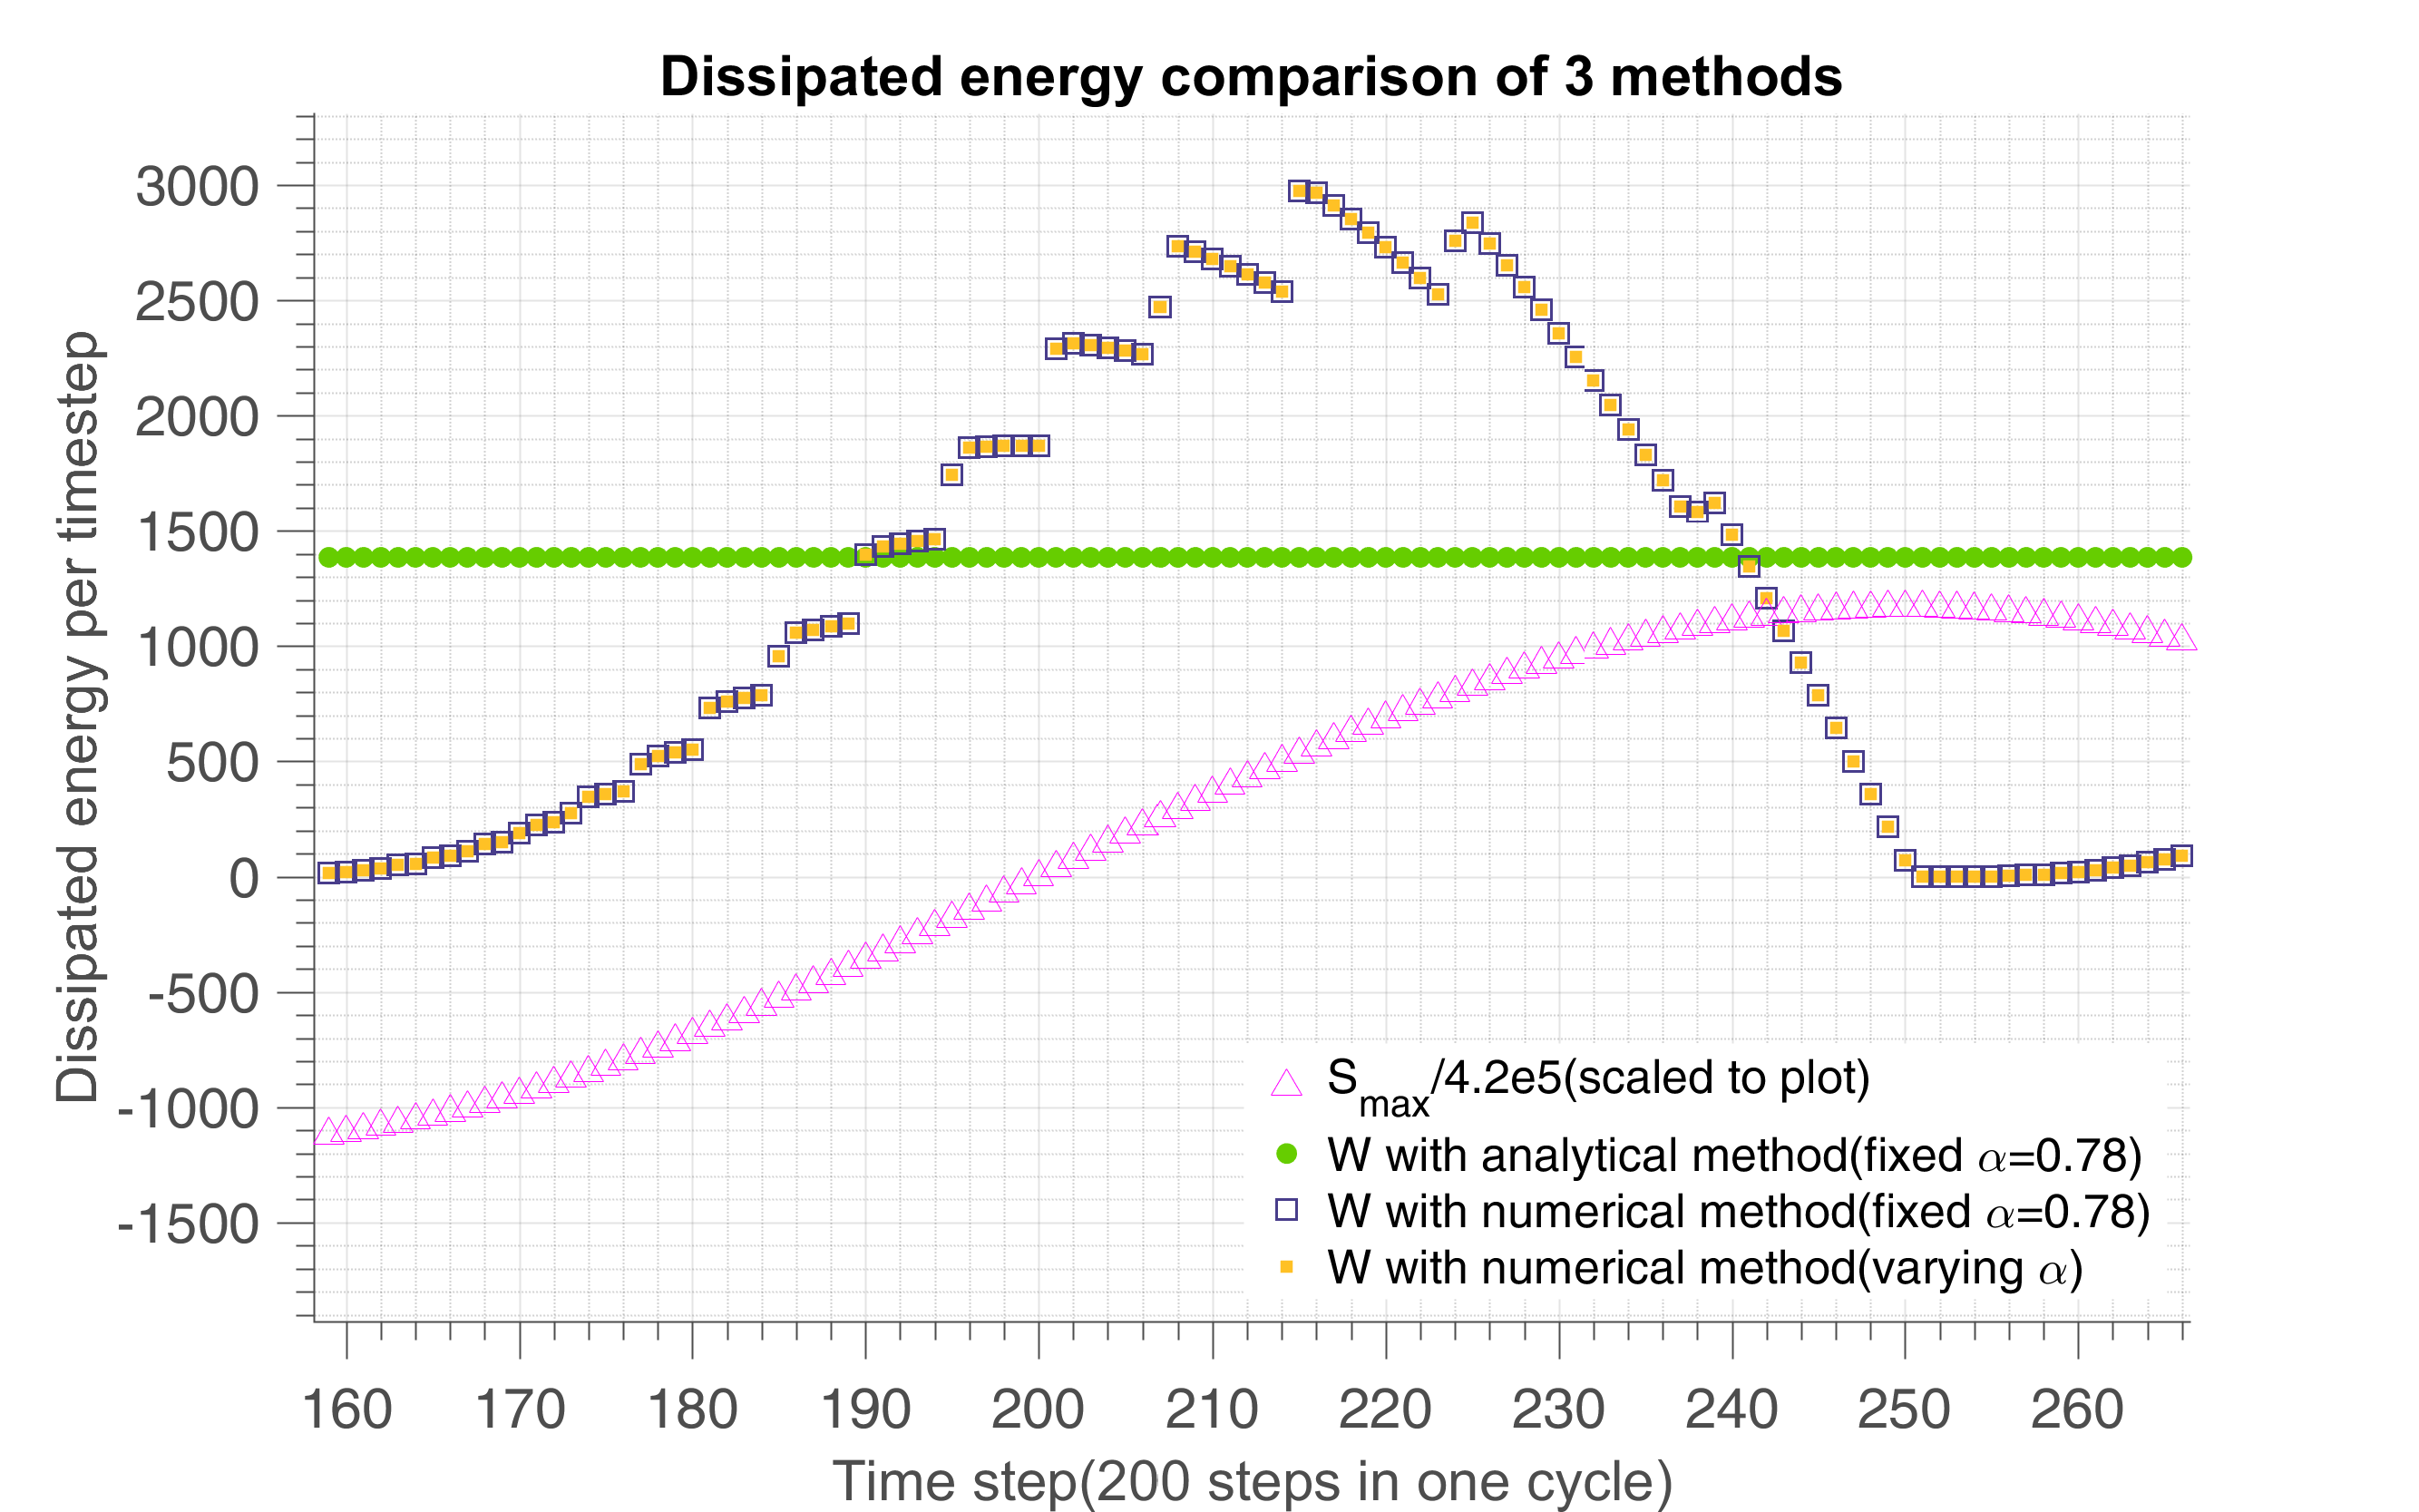
\includegraphics[width=0.95\textwidth]{figures//W_3methods_enlarge.png} 
	\caption{Validation of dissipated energy in all scales with analytical and numerical method(enlargement of \figref{fig.W3methods})}
	\label{fig.W3methodsenlarge}
\end{figure}
\begin{figure}[!h]
\centering
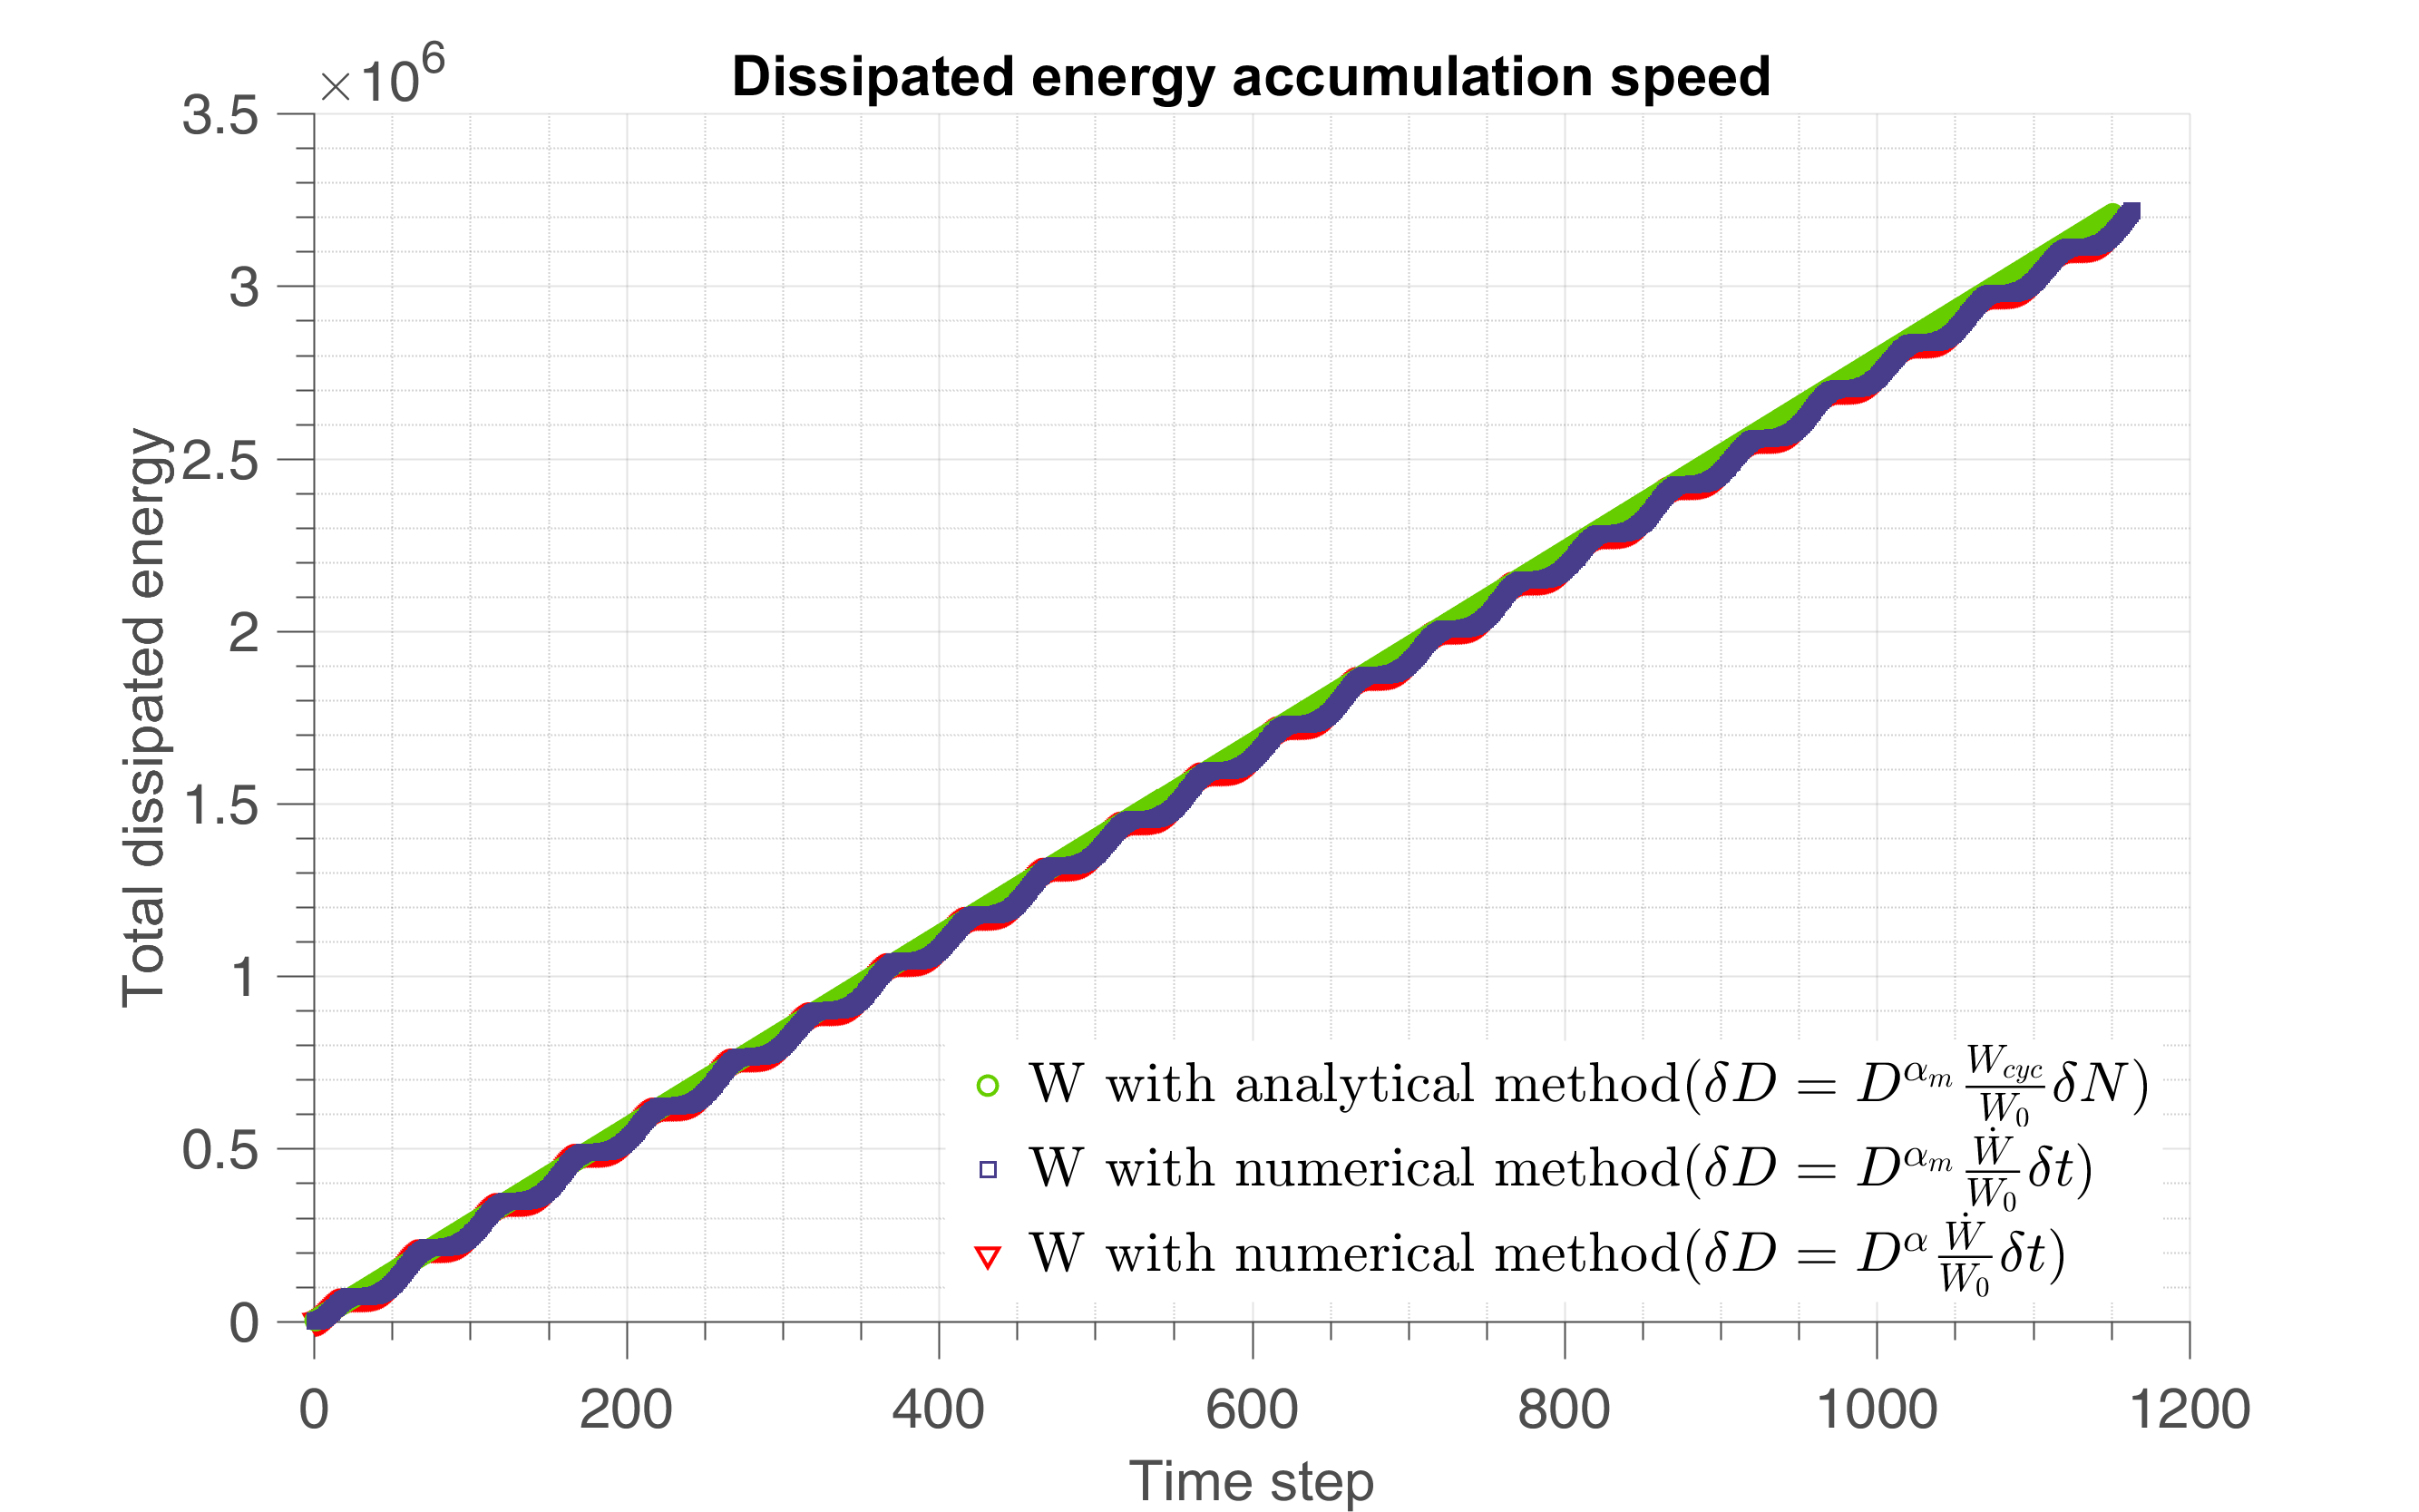
\includegraphics[width=0.95\textwidth]{figures//W_3methods2_100steps.png} 
\caption{Dissipated energy accumulation through time with different methods, there are 100 time steps in unit cycle}
\label{fig.W3methods100}
\end{figure}
\begin{figure}[!h]
\centering
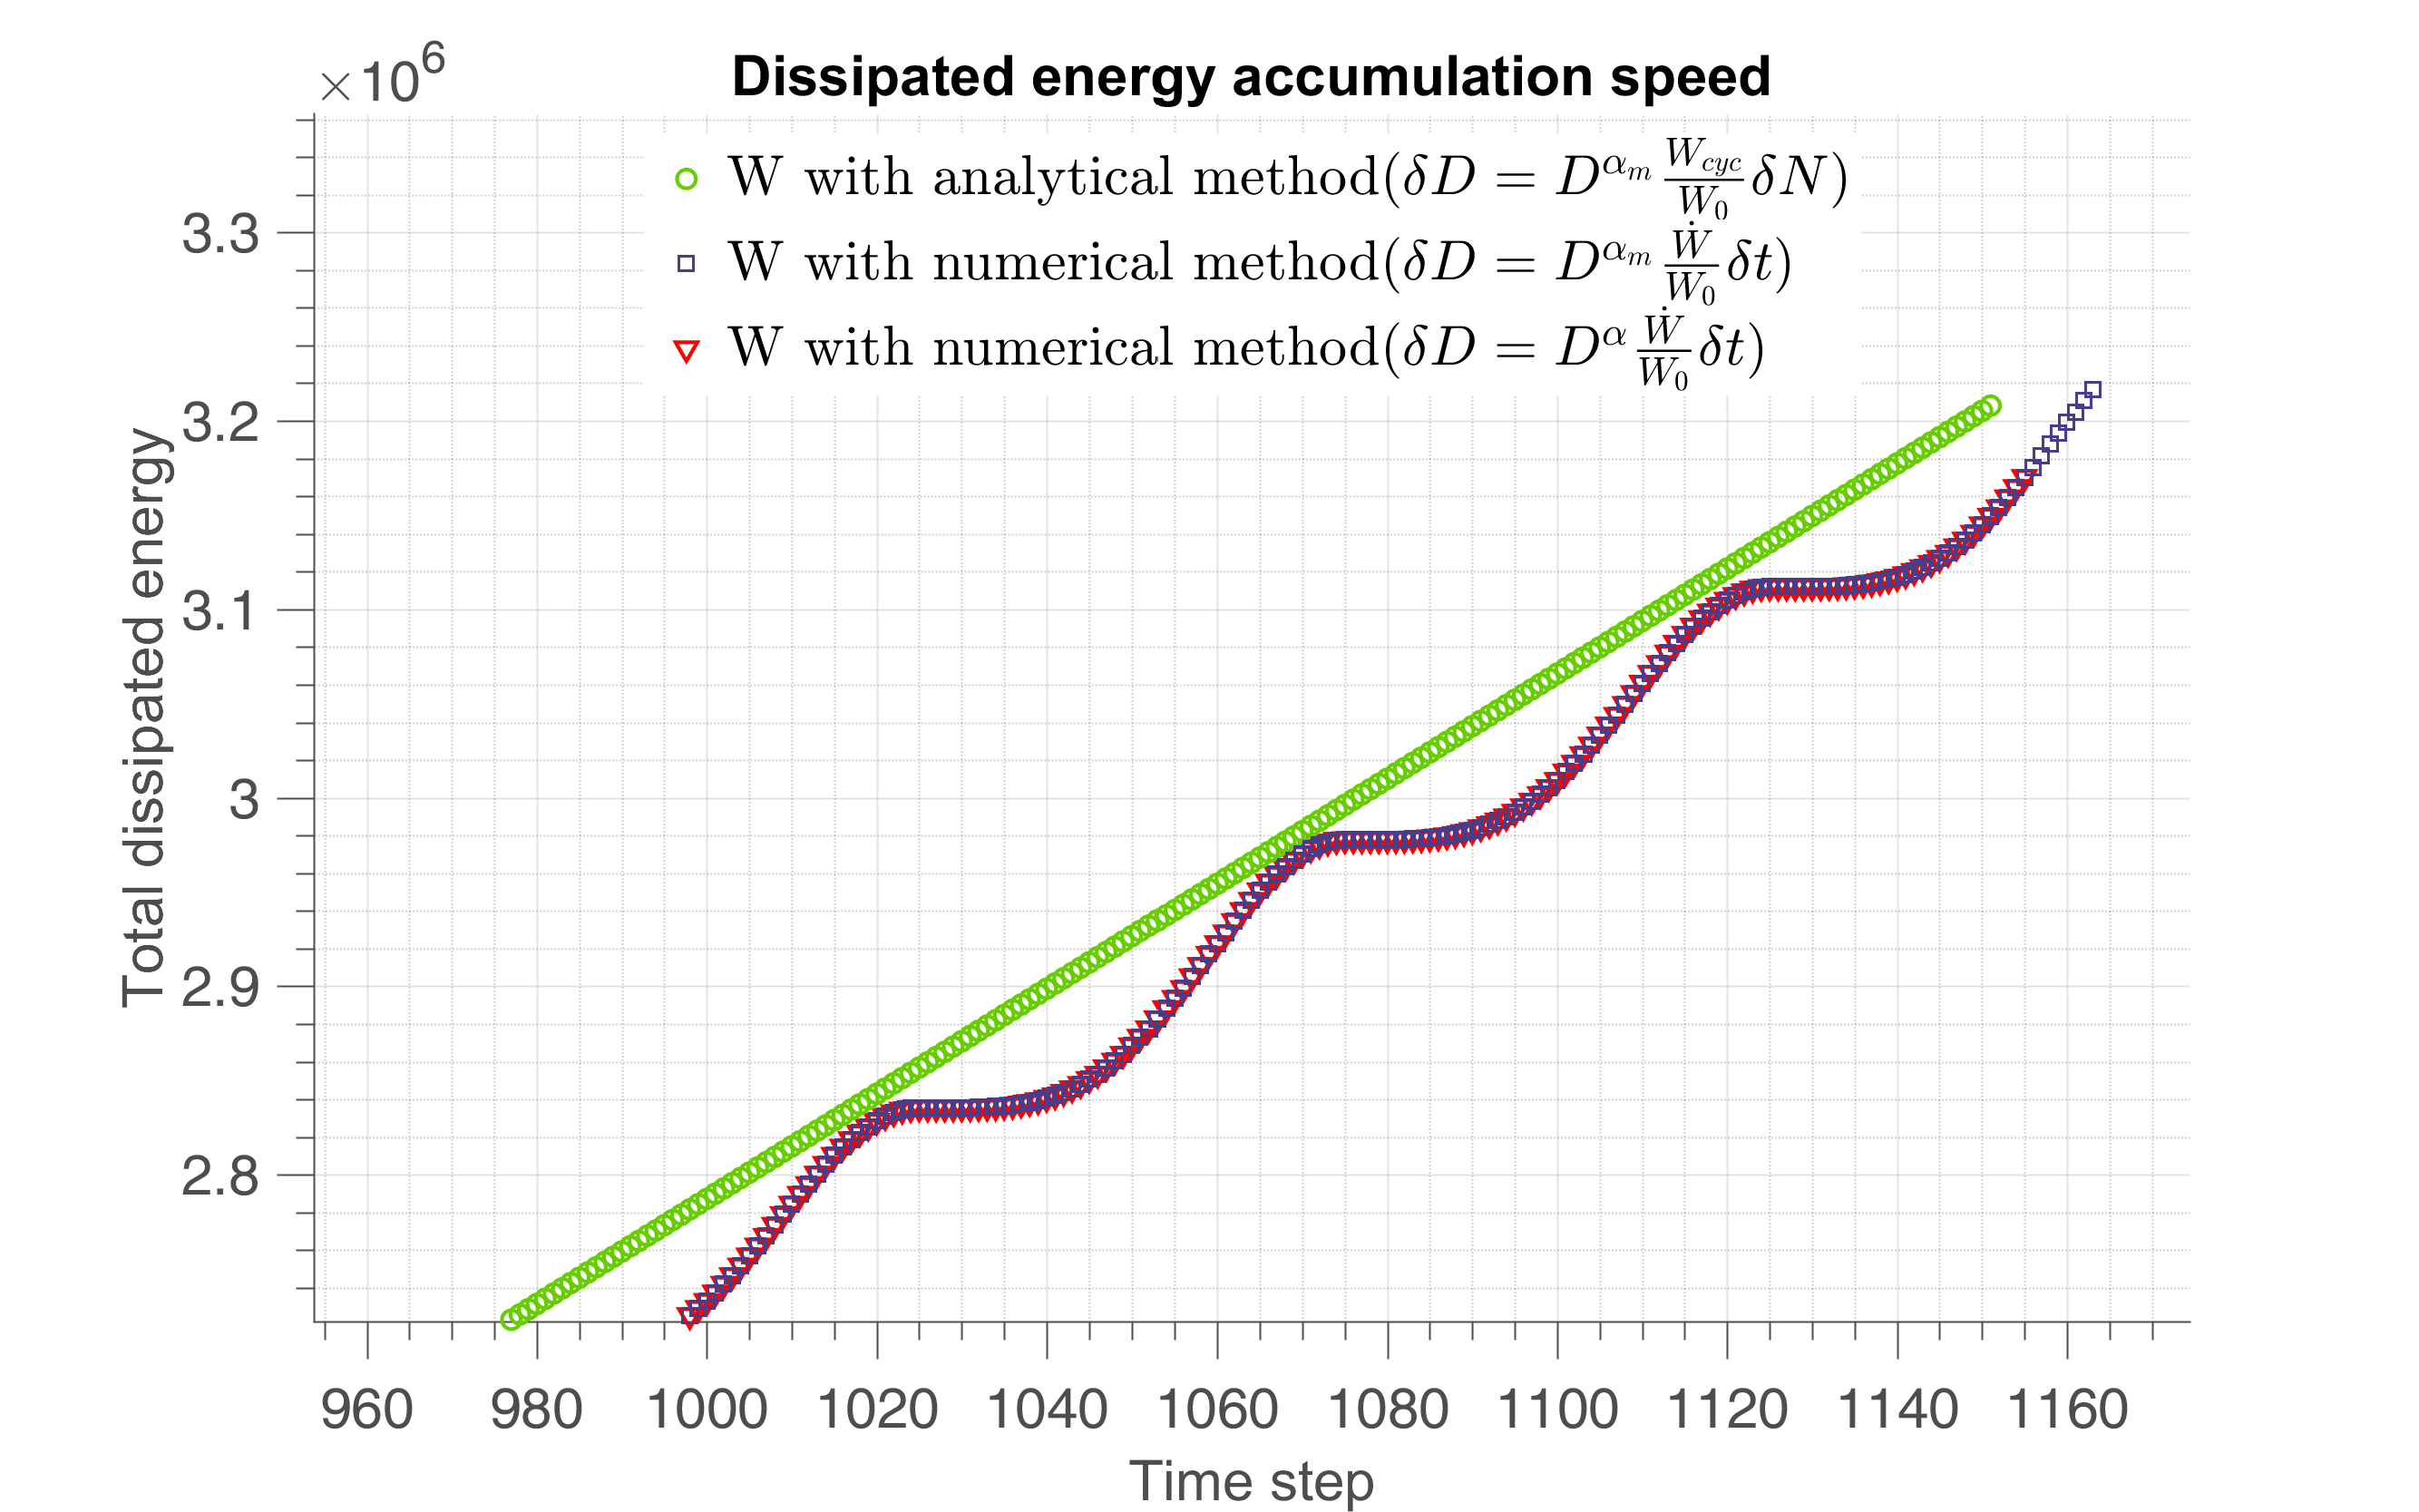
\includegraphics[width=0.95\textwidth]{figures//W_3methods_100steps_enlarge.png} 
\caption{Dissipated energy accumulation through time with of 3 methods(enlargement of \figref{fig.W3methods100})}
\label{fig.W3methods2enlarge}
\end{figure}
\begin{figure}[!h]
\centering
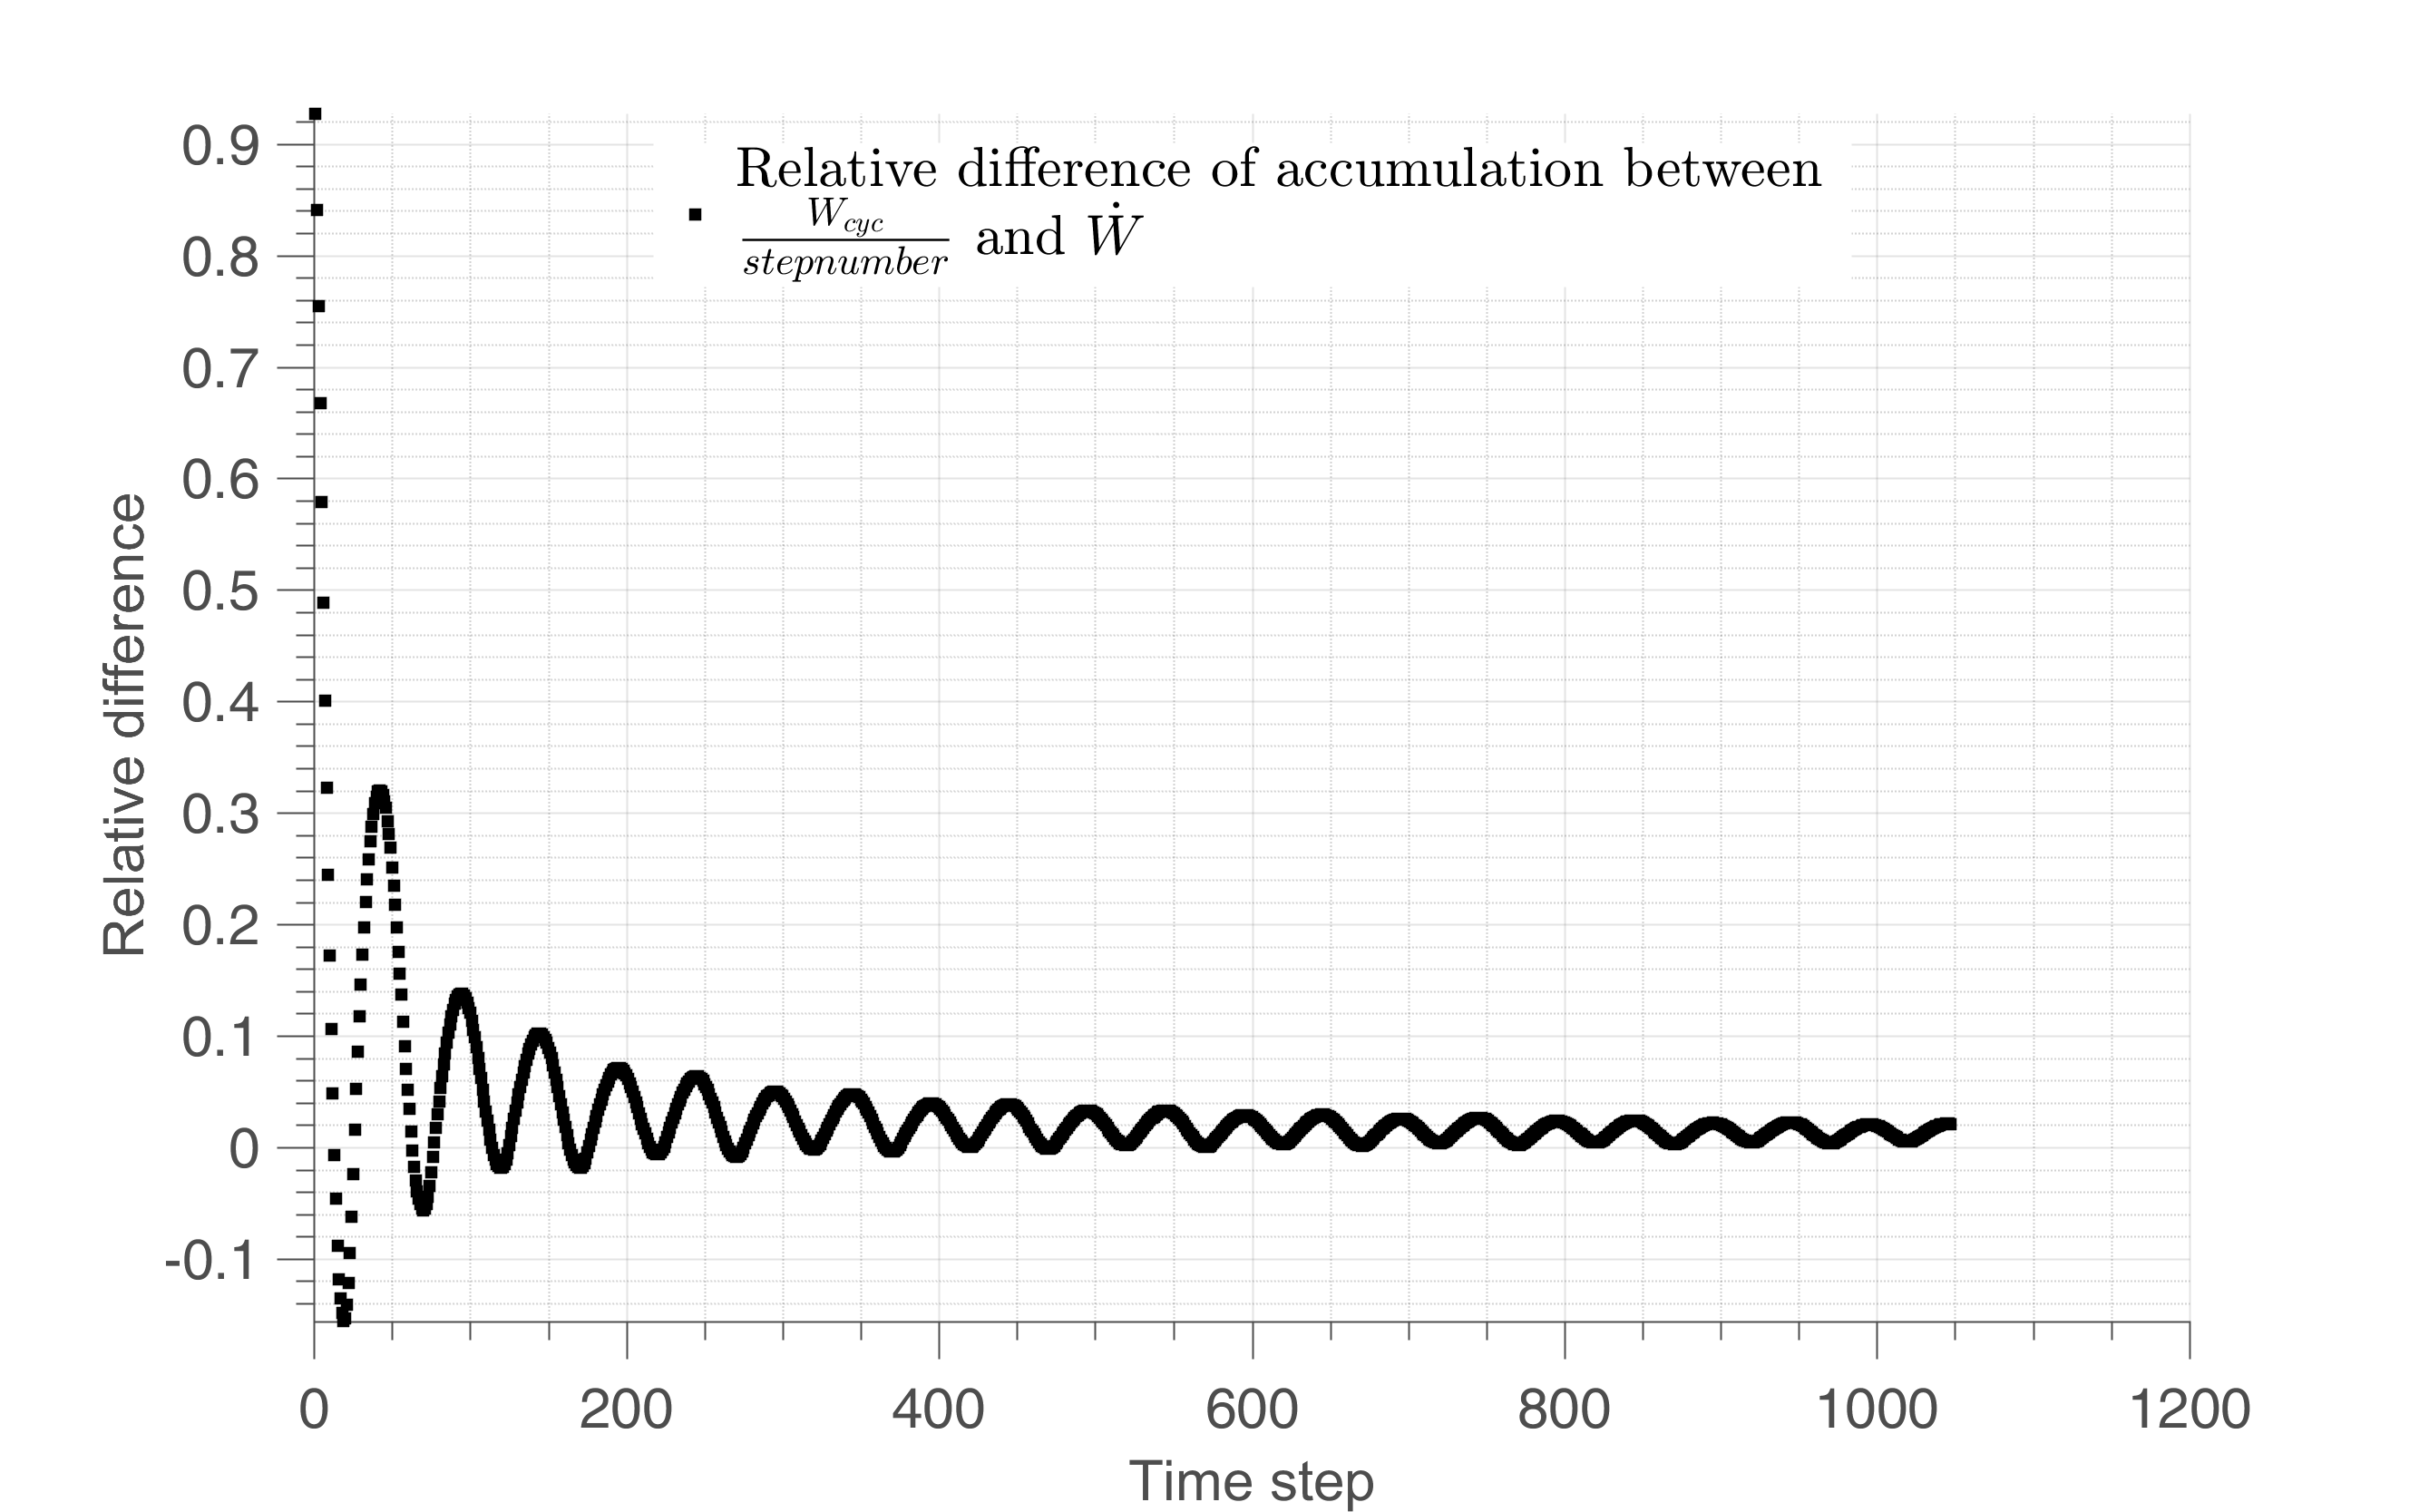
\includegraphics[width=0.95\textwidth]{figures//W_3methods_diff_100steps.png} 
\caption{Relative difference $\dfrac{W_{analytical}-W_{numerical}}{W_{analytical}}$ between analytical energy loss and numerical one with $\alpha$ varying with time of \figref{fig.W3methods100}}
\label{fig.W3methodsdiff}
\end{figure}
\begin{figure}[!h]
\centering
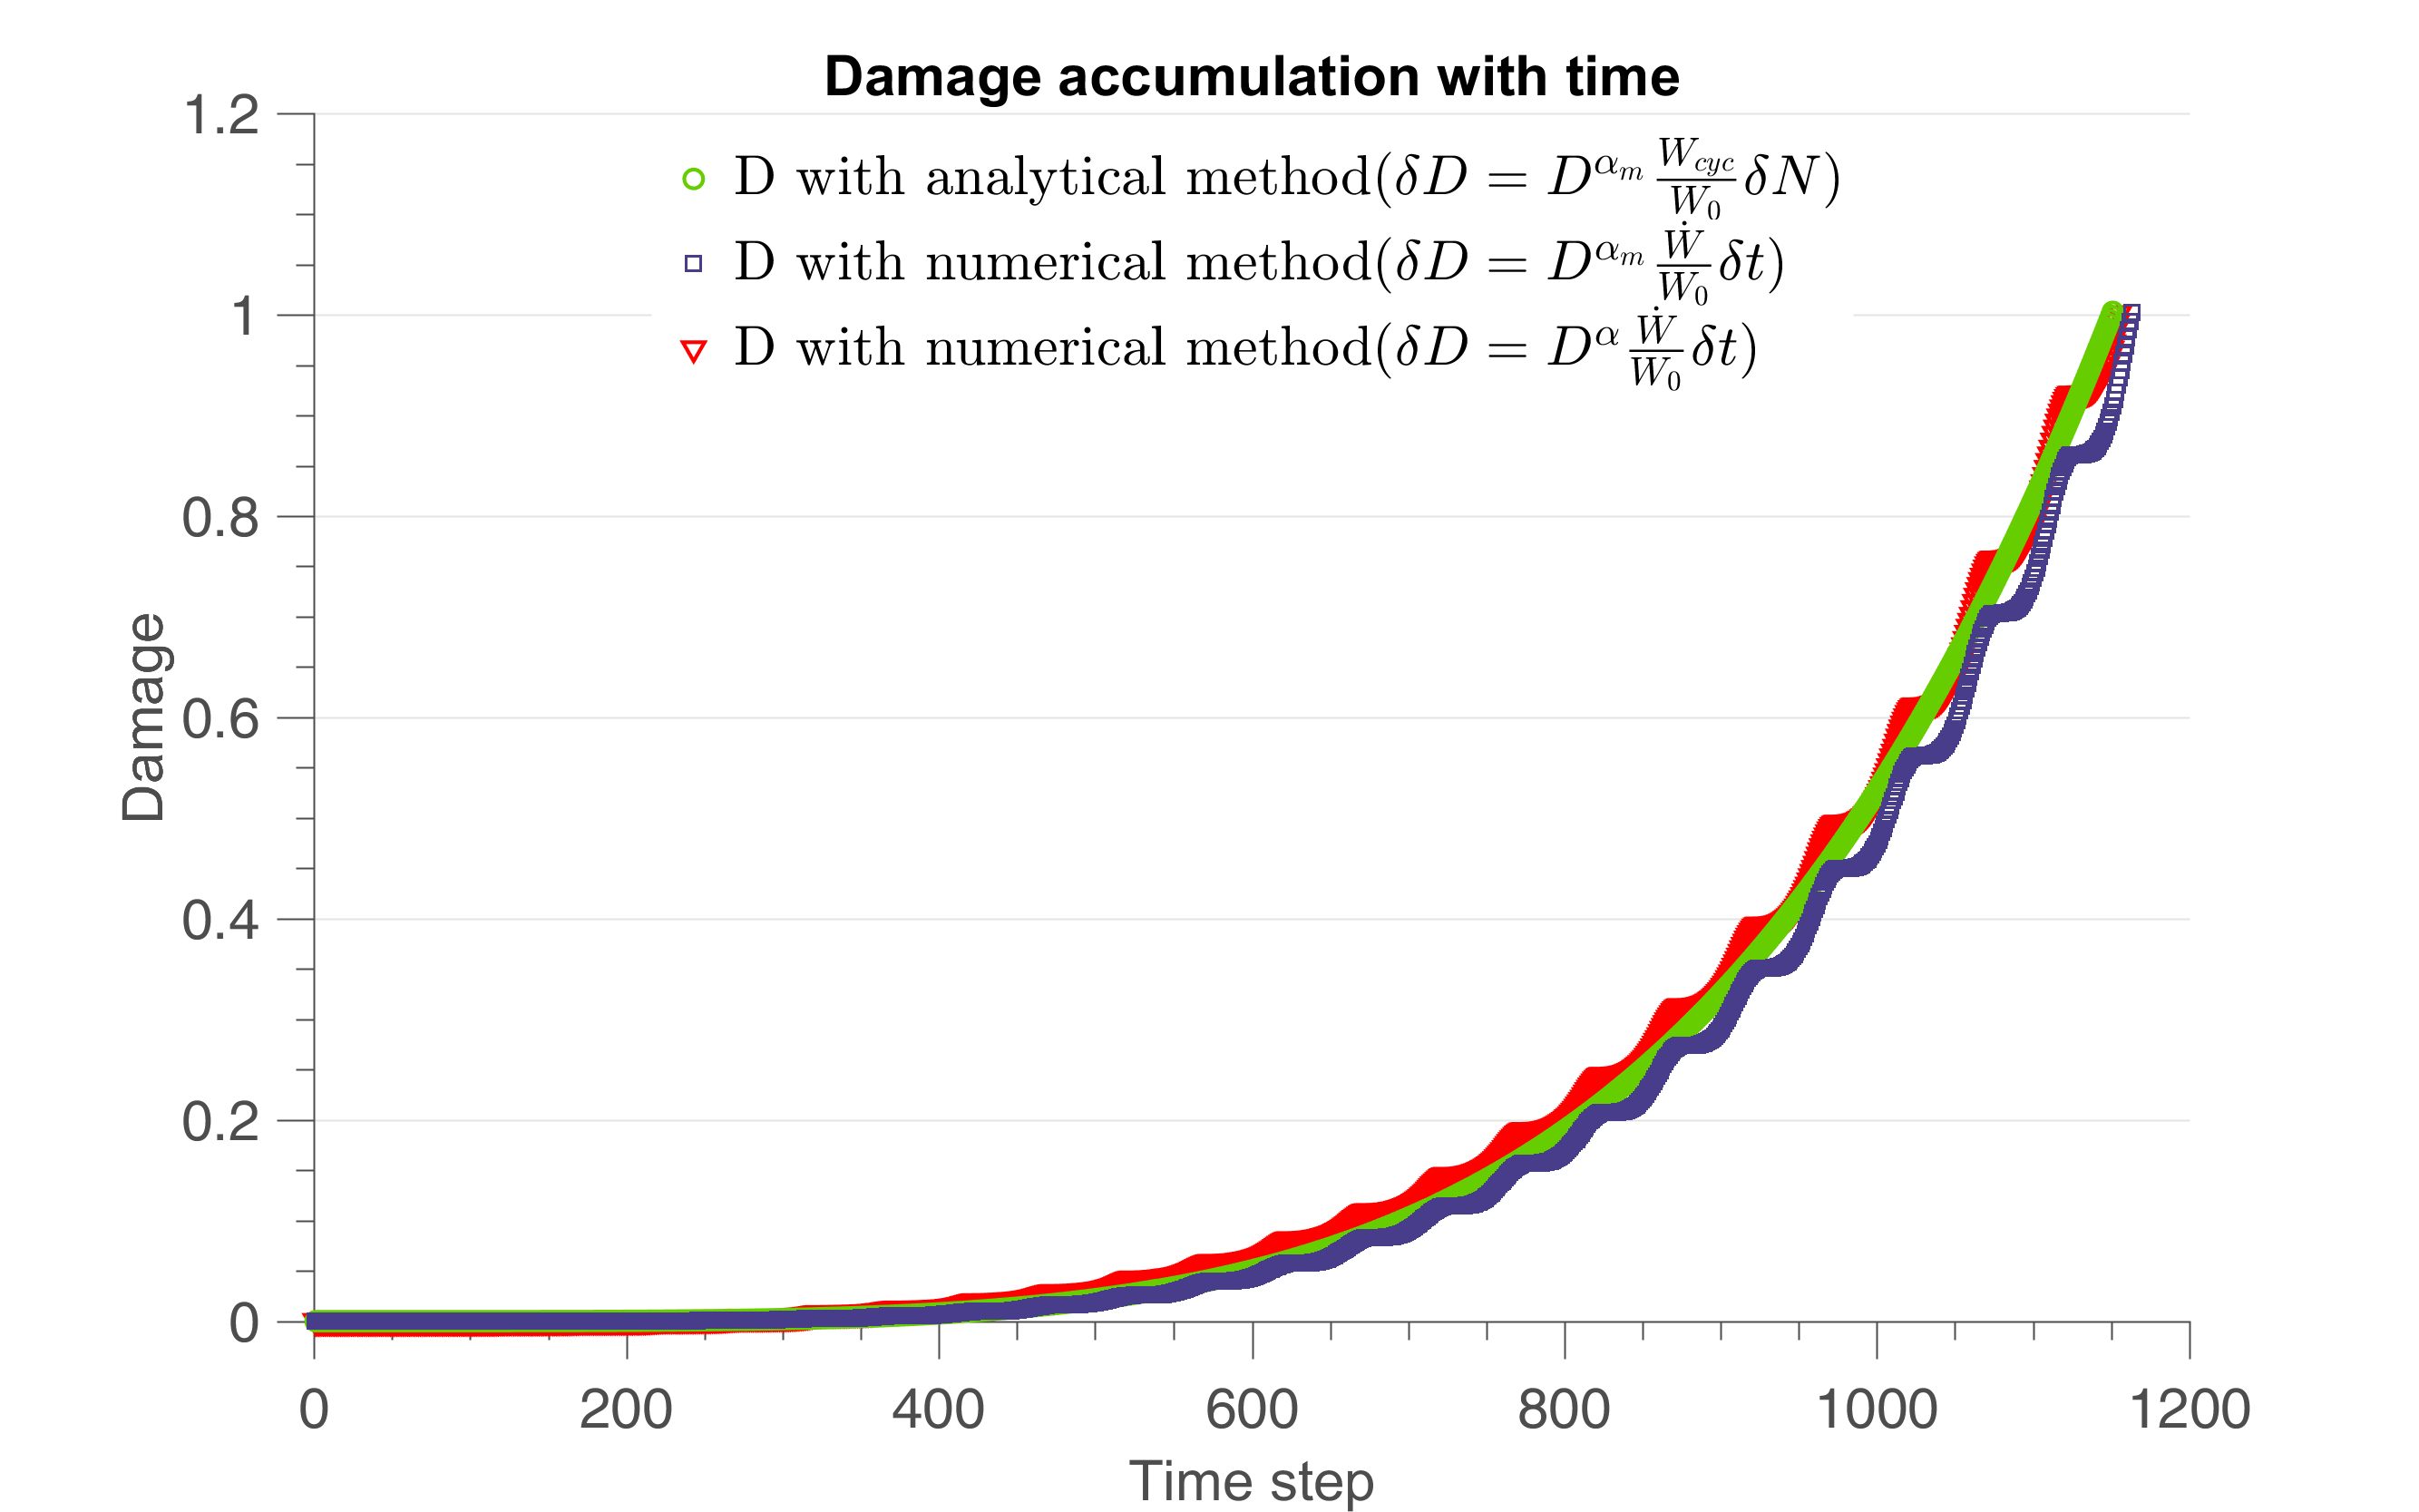
\includegraphics[width=\textwidth]{figures//D_3methods2_100steps.png} 
\caption{Damage evolution with time under sinusoidal load with different methods, there are 100 time steps in unit cycle($\beta=1.1$,$\Sigma=0.85\sigma_y$)}
\label{fig.damsin100}
\end{figure}

\begin{figure}[!h]
\centering
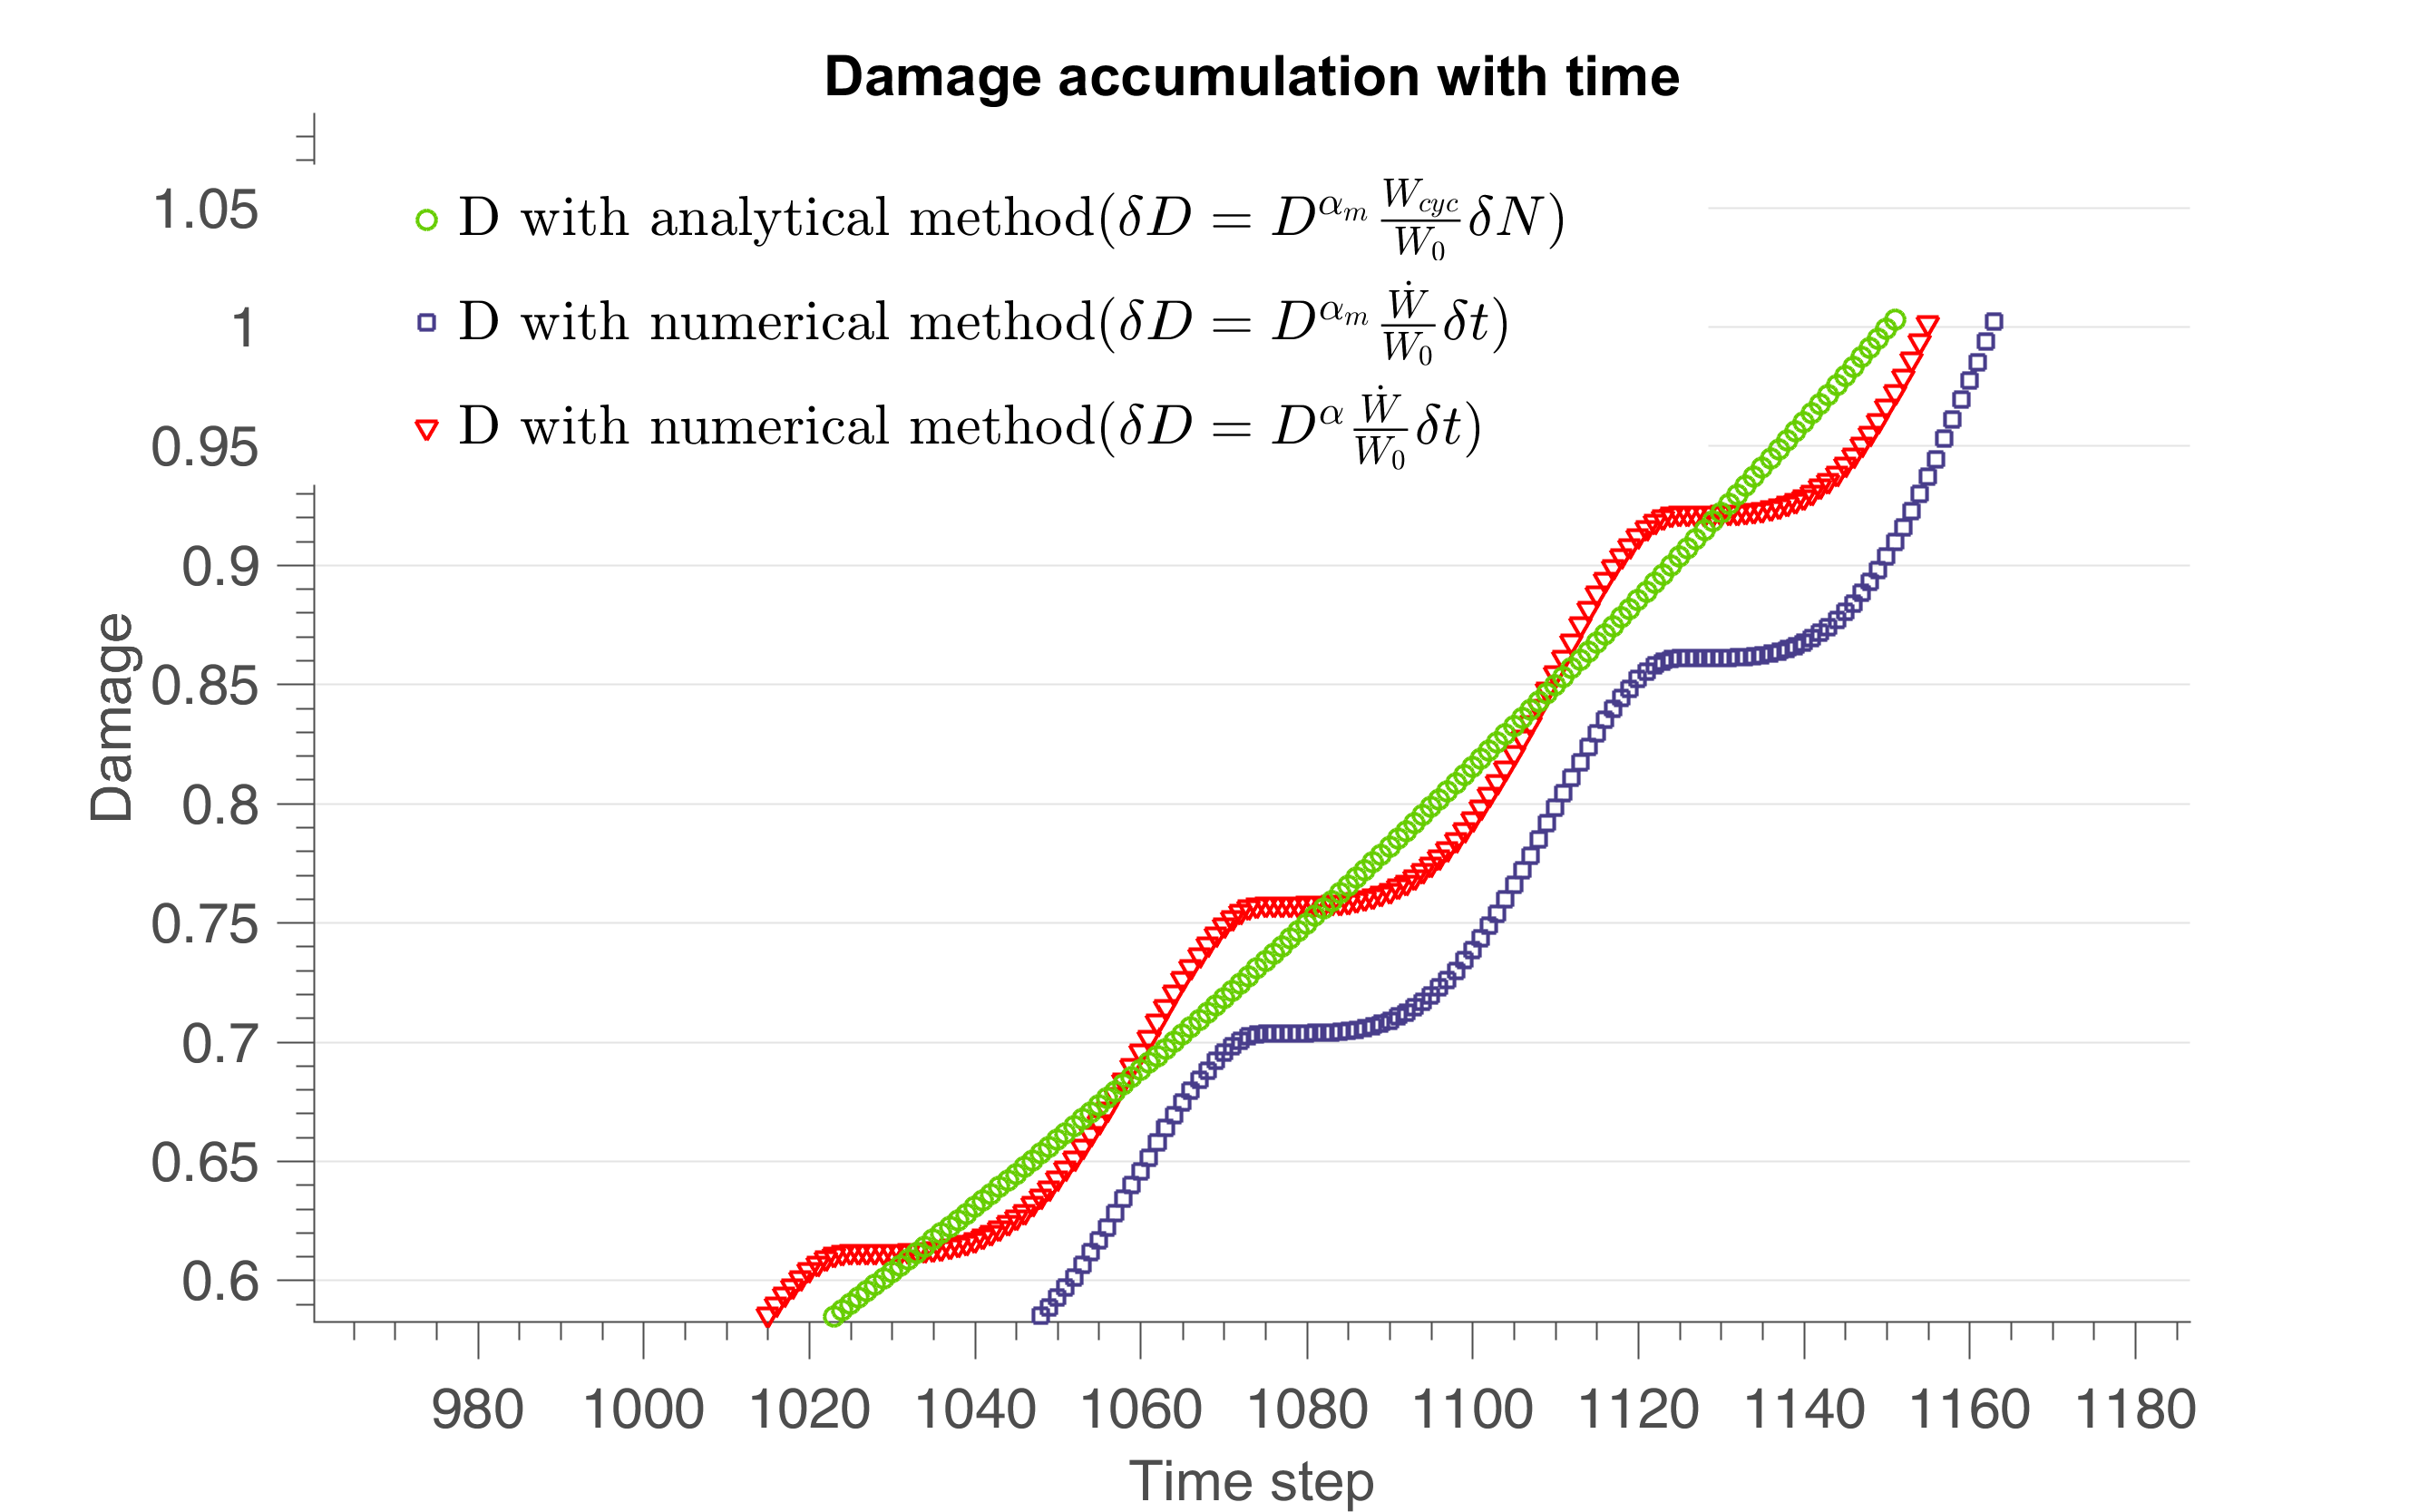
\includegraphics[width=\textwidth]{figures//D_3methods_100steps_enlarge.png} 
\caption{Damage evolution with time under sinusoidal load with two different methods(enlargement of \figref{fig.damsin100})}
\label{damsinenglarge}
\end{figure}

\begin{figure}[!h]
\centering
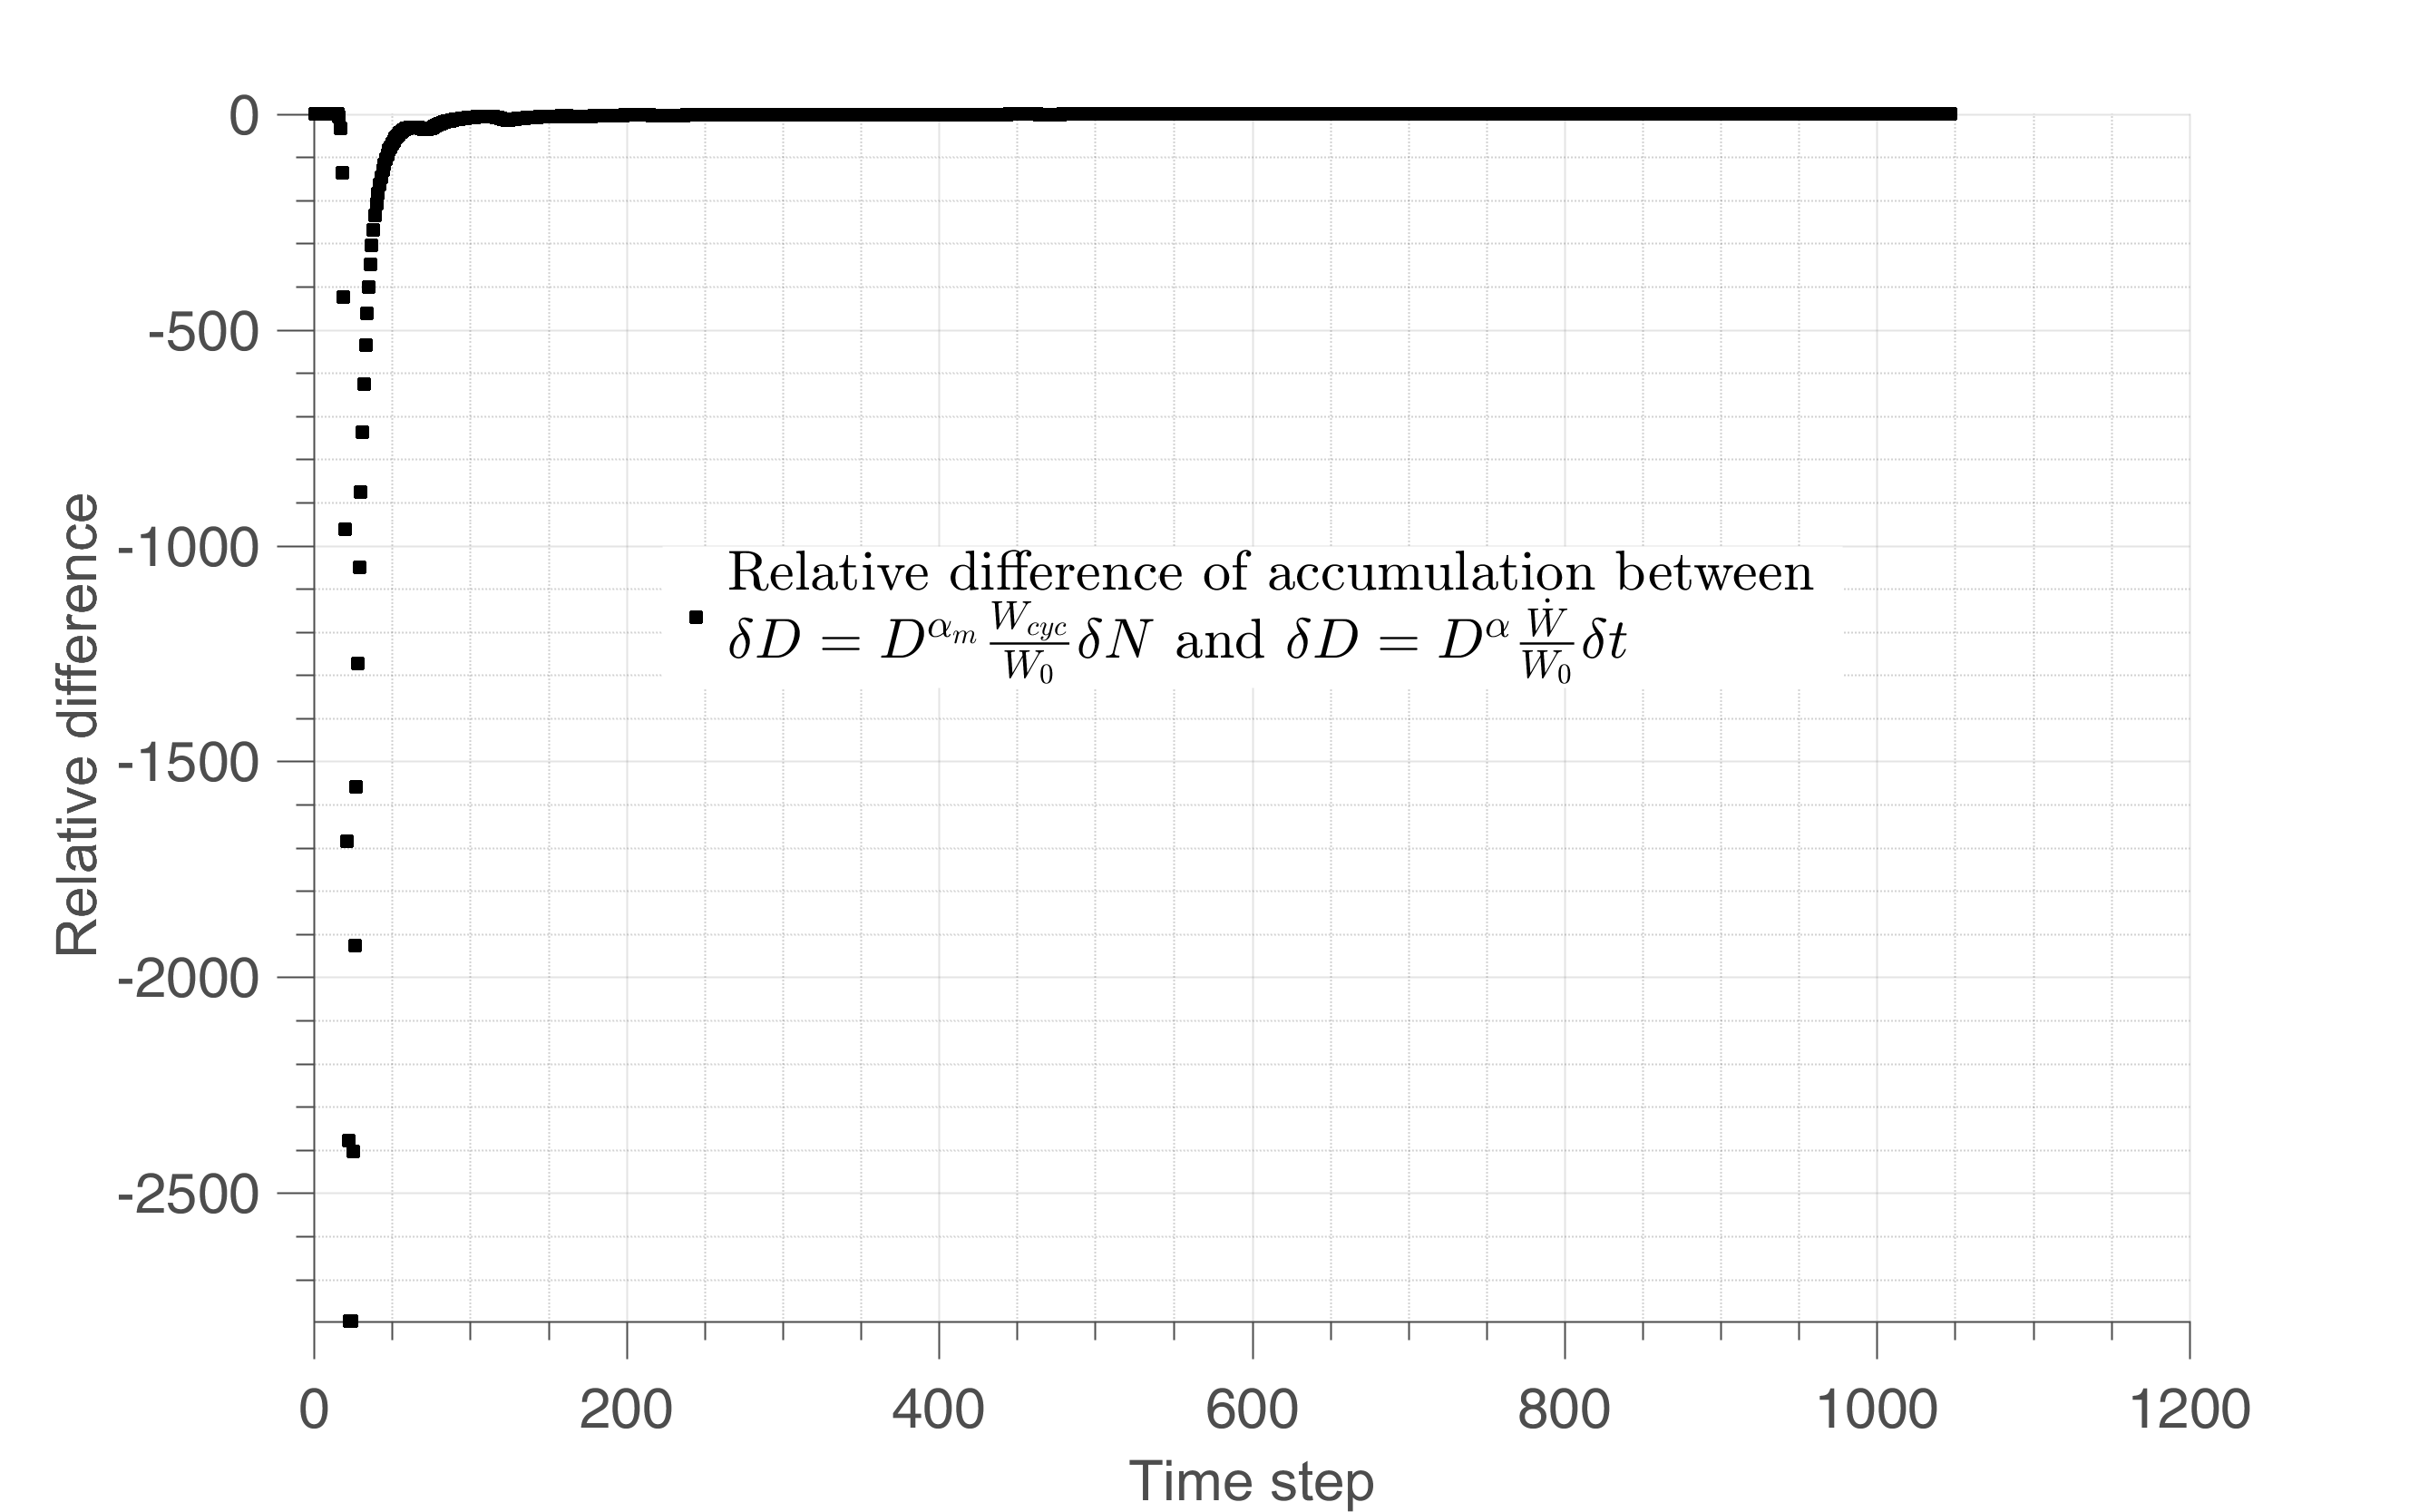
\includegraphics[width=\textwidth]{figures//D_3methods_diff_100steps.png} 
\caption{Relative difference $\dfrac{D_{analytical}-D_{numerical}}{D_{analytical}}$ evolution with time of \figref{fig.damsin100}}
\label{Damagediff}
\end{figure}
We take the mean value of $\alpha$ during all the iteration process of numerical method as $\alpha_{m}$. The energy and damage accumulation is shown in \figref{fig.W3methods100} and \figref{fig.damsin100}. Here we give 100 time steps in one cycle to see the relative difference between changing $\alpha$ and $\alpha_{m}$, also $\dot{W}$ and $W_{cyc}/stepnumber$  method. The more time steps we give, the more precision we get. The relative difference between analytical energy loss and numerical one is shown in \figref{fig.W3methodsdiff} from which we conclude that the three methods converge in terms of elastic energy dissipation, but due to nonlinear effects the damage evolution does not have the same history per cycle. The frozen $\alpha$ delays damage, the varying $\alpha$ increases damage during the phase of strong loading. The difference has a significant impact if damage occurs with very few cycles. It will not when computing on a large number of cycles.

The cyclic load calculation is only valid for very simple such as proportional loading in fatigue. However, the convergence of the two methods is based on the small value of $\beta$(close to 1), in case of large values of $\beta$(typically around 5), the numerical strategy gives shorter life than the analytical one due to extreme non-linearity in the energy dissipation history per cycle. The relative error is around 20\% as shown in \figref{fig.W3methods_bigbeta_04y} and \figref{fig.W3methods_bigbeta_08y}. Nevertheless the analytical formula can still be used as a comparison group to verify the numerical results. And in the identification process we need the analytical form to fit the $S-N$ curve of a certain material. The outcome is satisfactory. Hence, to be more general for any loading history, we adopt the numerical method after identification of $\beta$. 

\begin{figure}[!h]
	\centering
	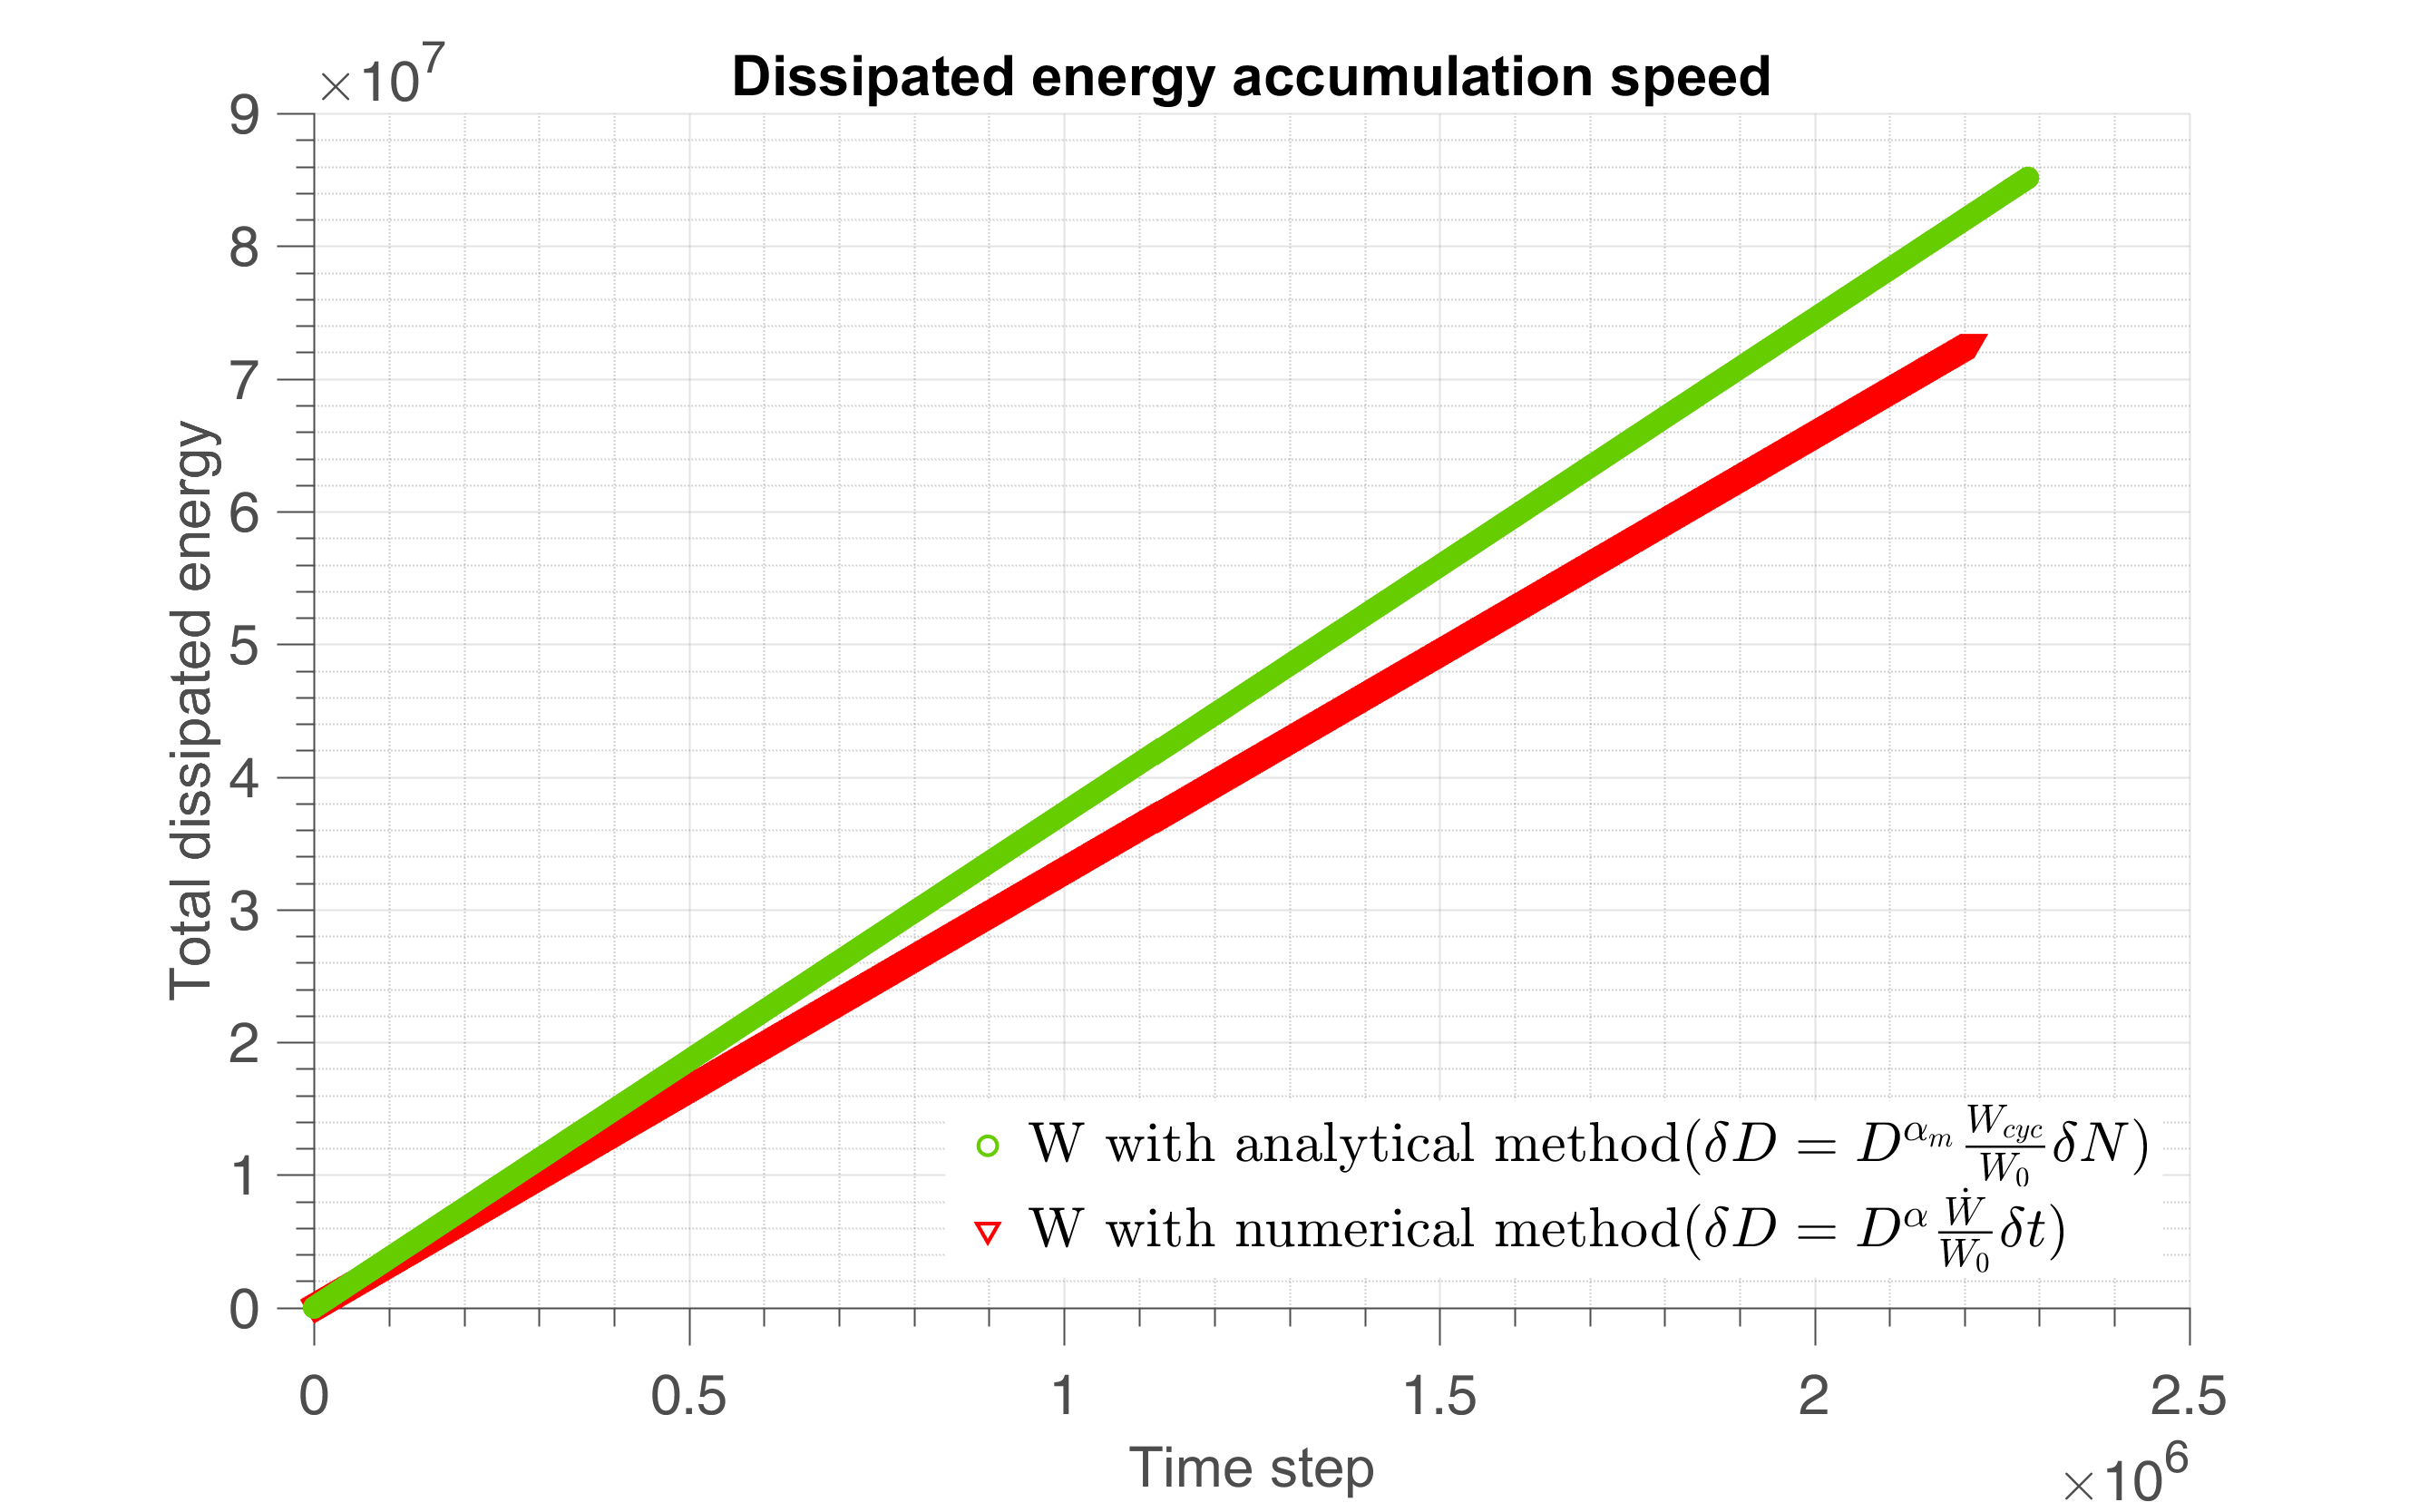
\includegraphics[width=0.95\textwidth]{figures//W3methods_bigbeta_04y.png} 
	\caption{Validation of dissipated energy in all scales with analytical and numerical method with $\beta=5$, $\Sigma=0.4\sigma_y$ }
	\label{fig.W3methods_bigbeta_04y}
\end{figure}
\begin{figure}[!h]
	\centering
	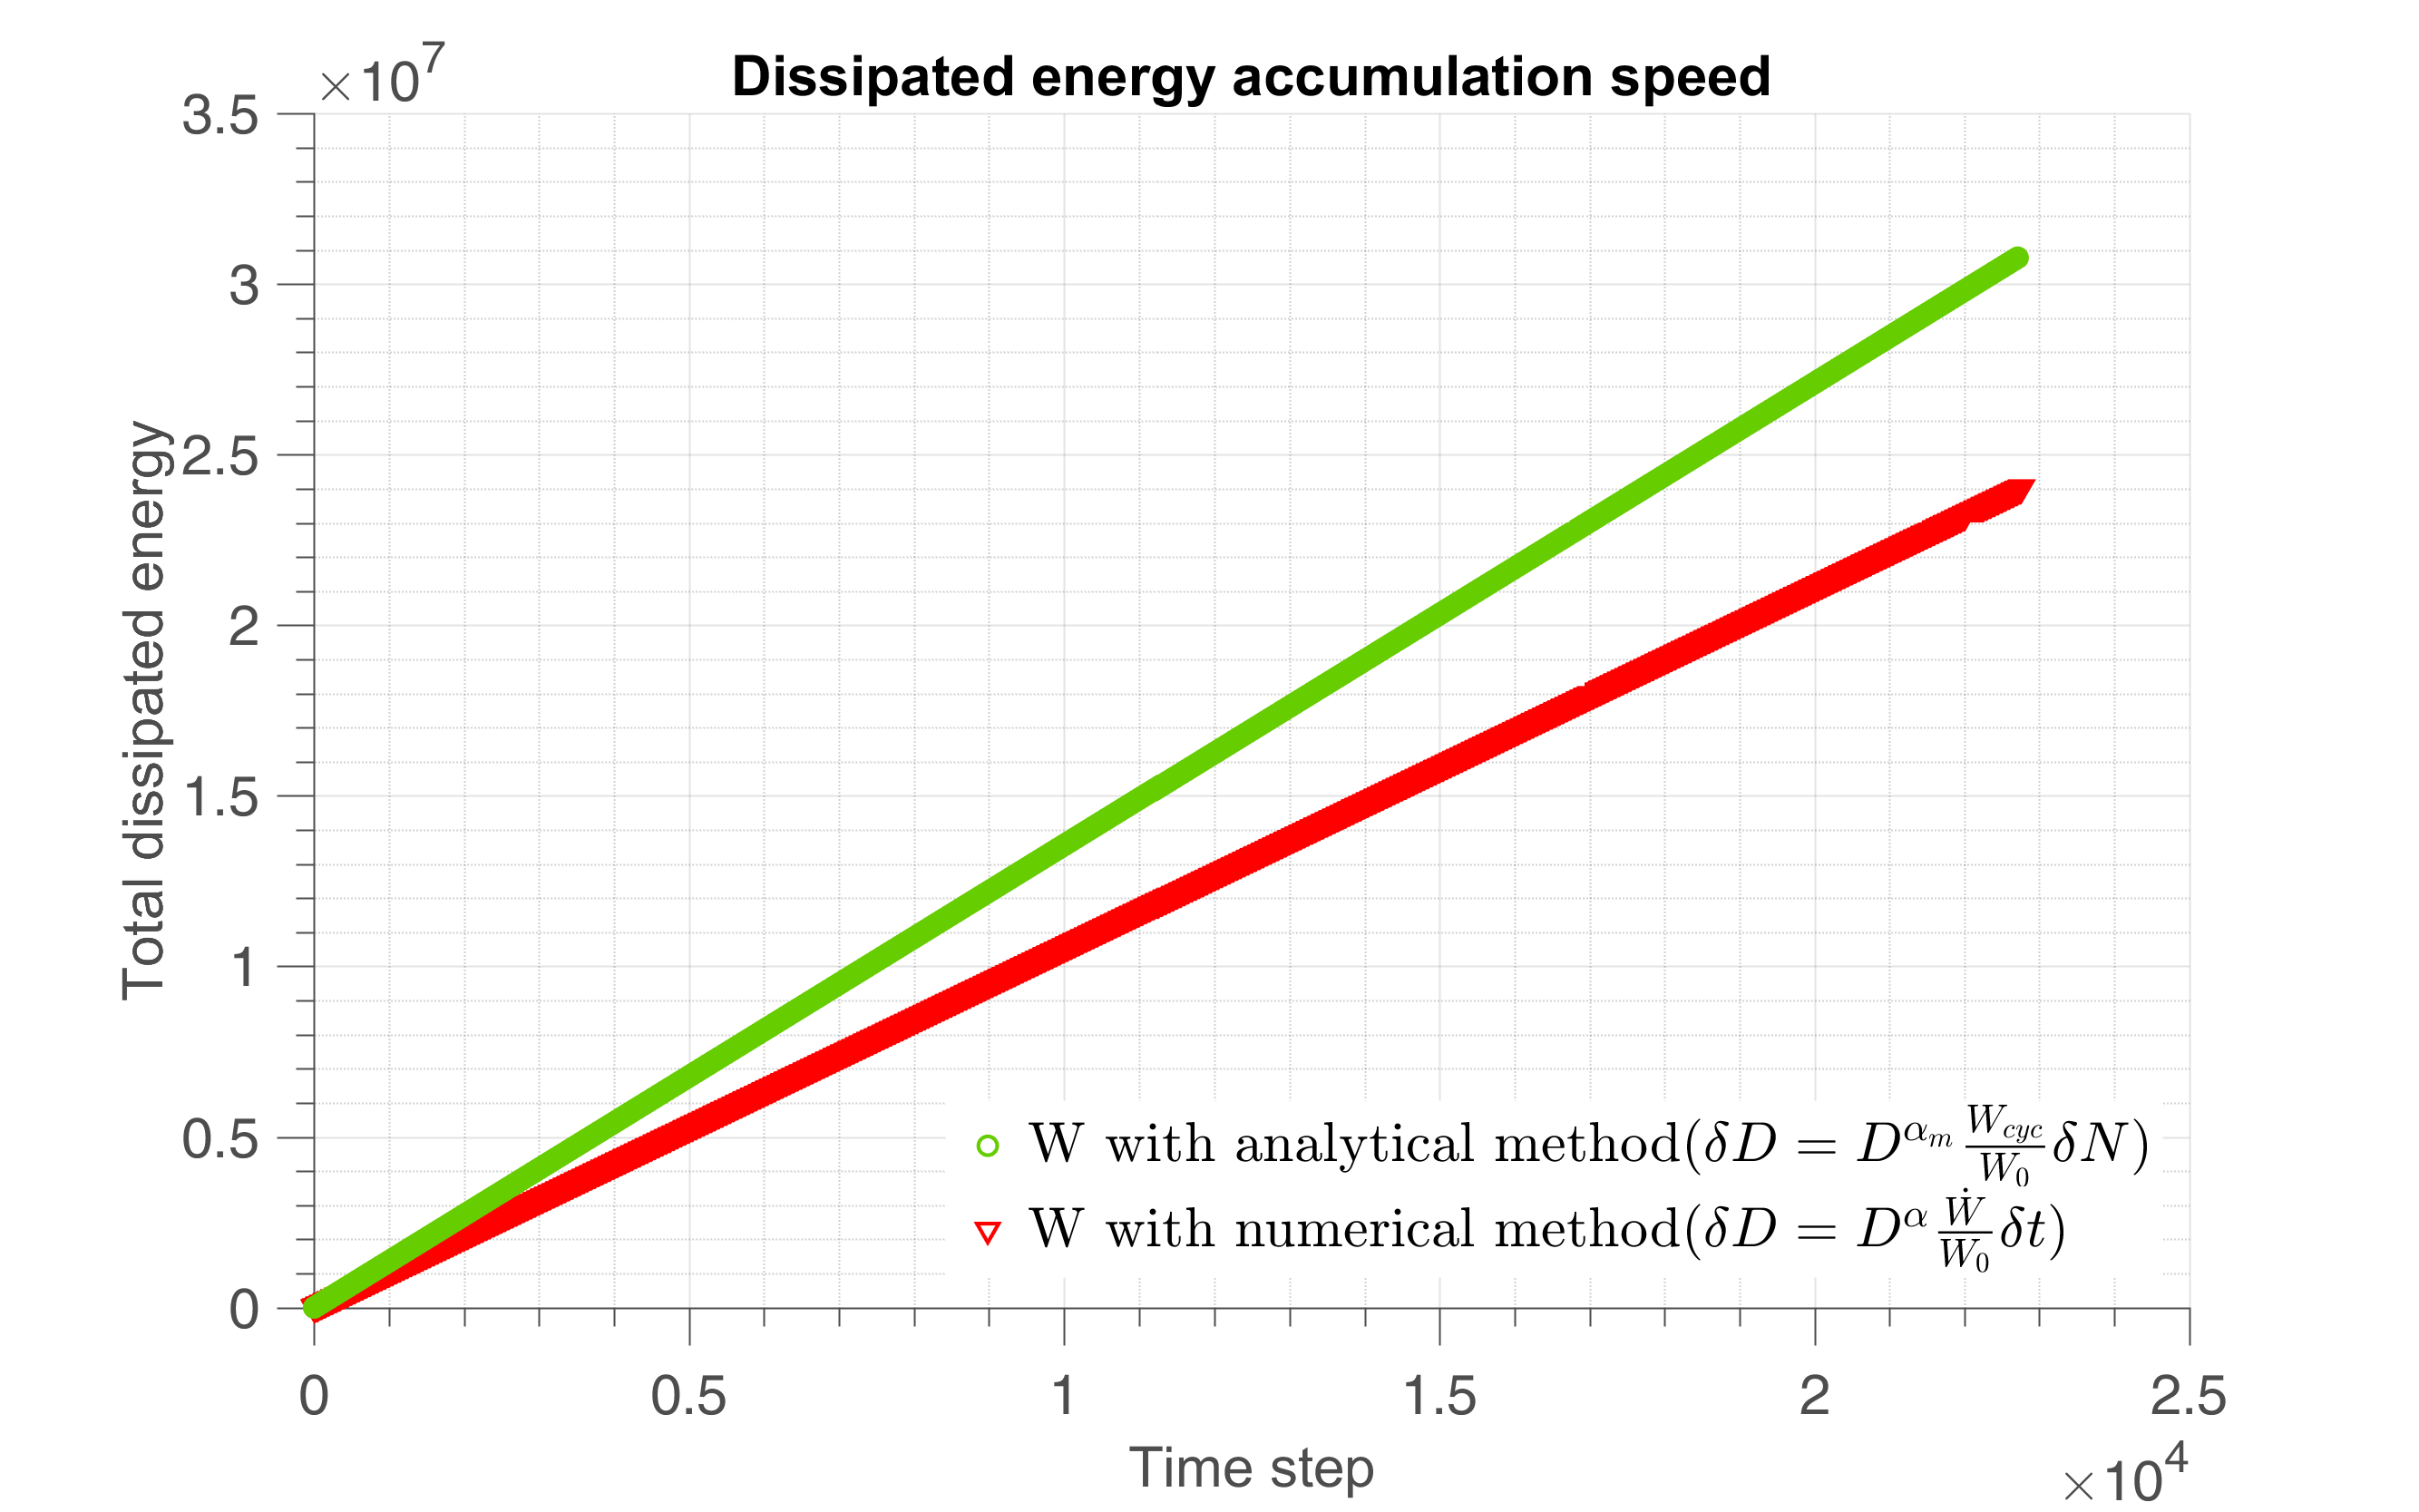
\includegraphics[width=0.95\textwidth]{figures//W3methods_bigbeta_08y.png} 
	\caption{Validation of dissipated energy in all scales with analytical and numerical method with $\beta=5$, $\Sigma=0.8\sigma_y$ }
	\label{fig.W3methods_bigbeta_08y}
\end{figure}
\begin{figure}[!h]
	\centering
	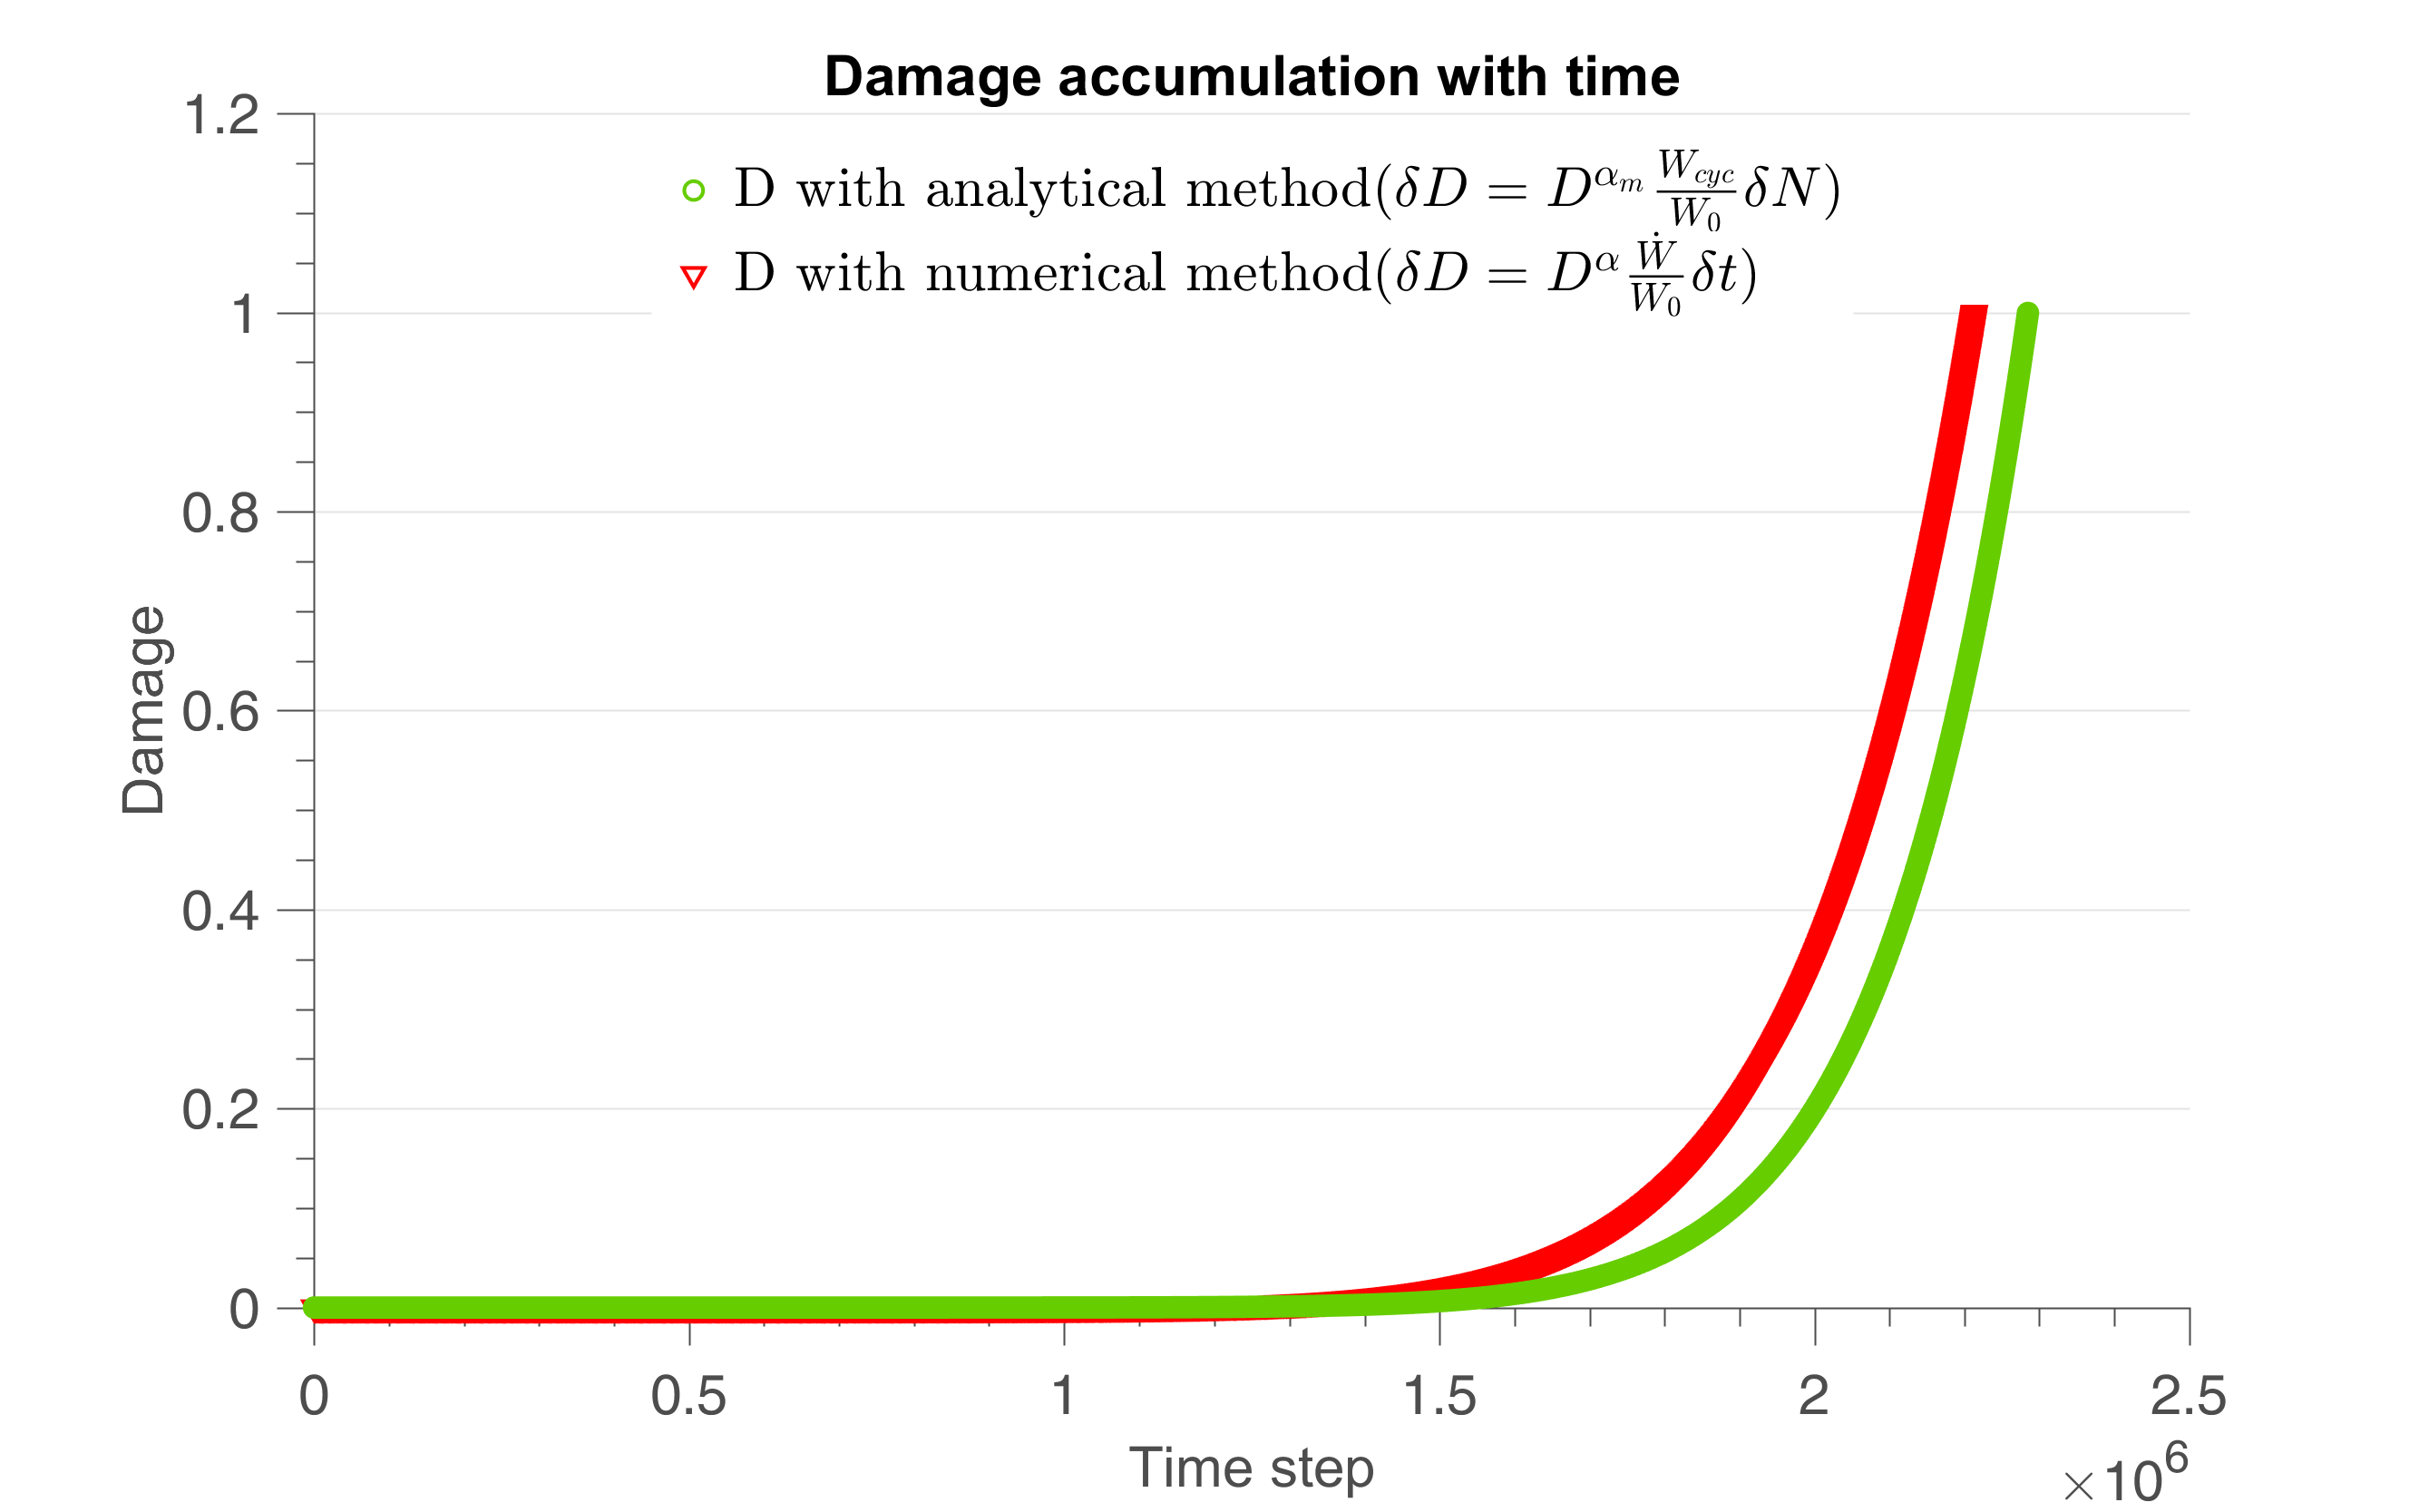
\includegraphics[width=\textwidth]{figures//damsin_bigbeta_04y.png} 
	\caption{Damage evolution with time under sinusoidal load with $\beta=5$, $\Sigma=0.4\sigma_y$. In such a severe loading and with extreme non-linearity, the simple Chaboche like formula with frozen $\alpha$ departs from the outcome of the full numerical model}
	\label{fig.damsin_bigbeta_04y}
\end{figure}
\begin{figure}[!h]
	\centering
	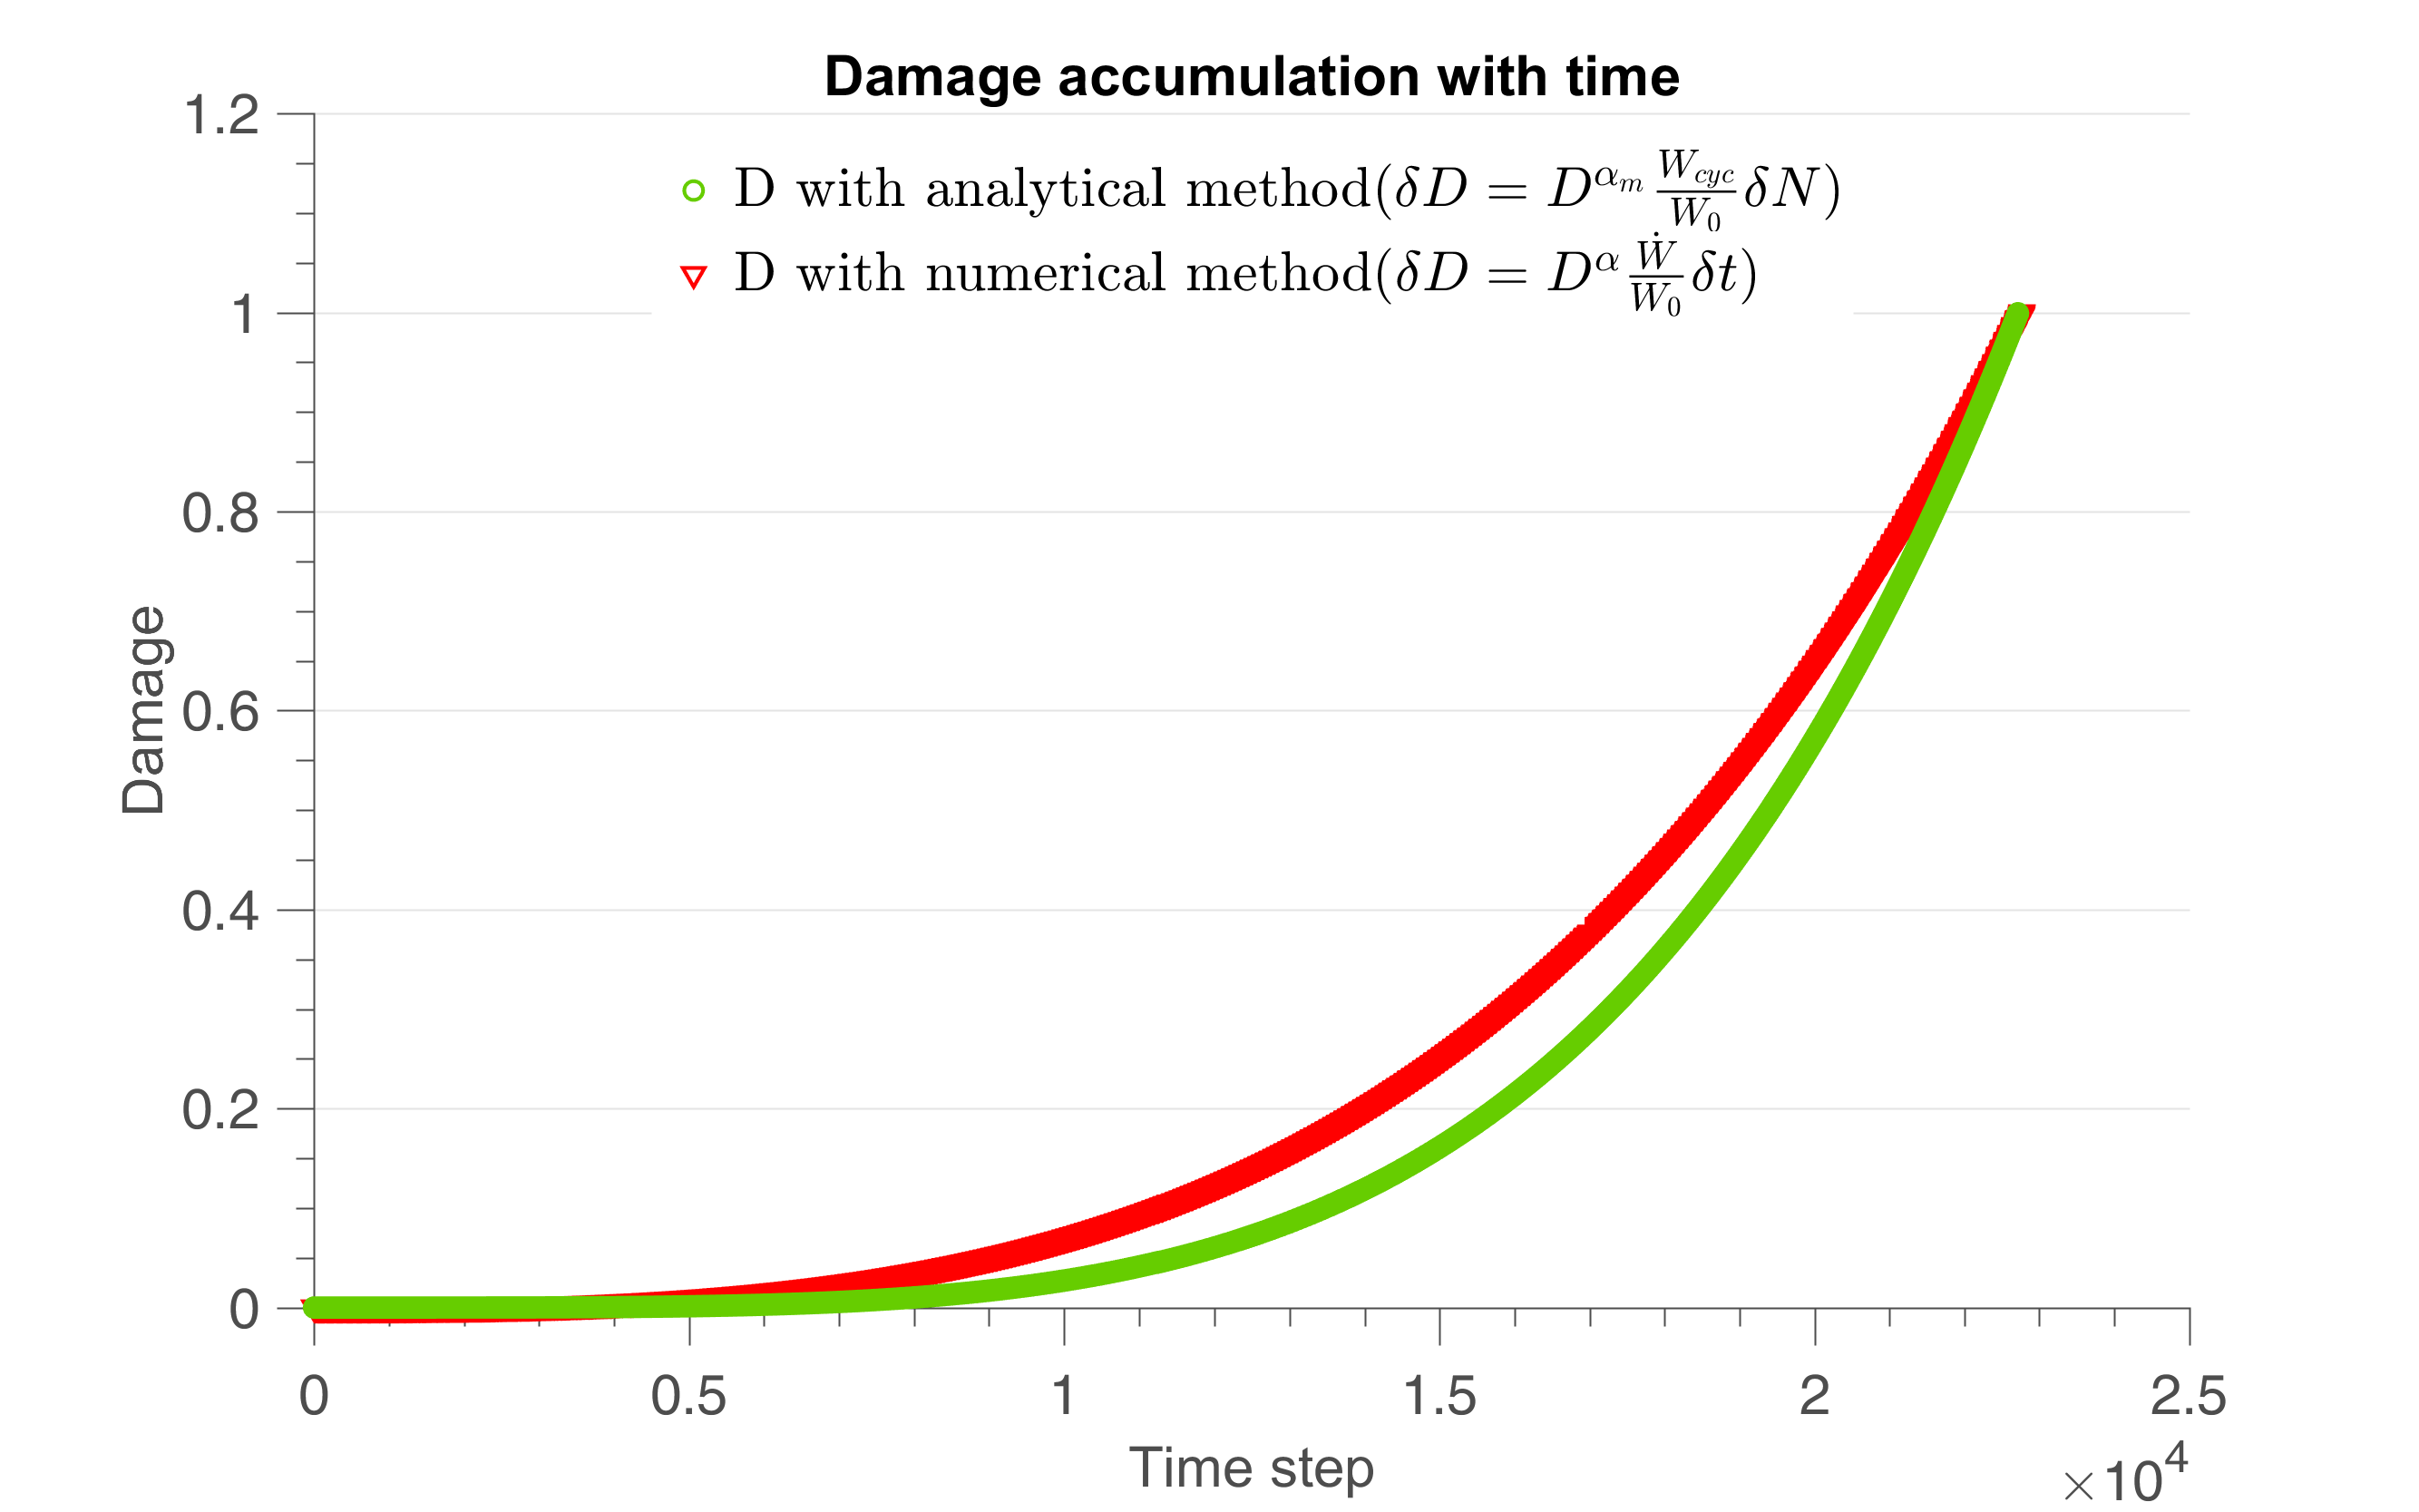
\includegraphics[width=\textwidth]{figures//damsin_bigbeta_08y.png} 
	\caption{Damage evolution with time under sinusoidal load with $\beta=5$, $\Sigma=0.8\sigma_y$}
	\label{fig.damsin_bigbeta_08y}
\end{figure}

\clearpage
\subsection{Numerical recovery of sequence effect}
We adopt the parameter $\alpha$ to take into account the sequence effect. The high-low loading sequence clearly reduces the fatigue life, as depicted in \figref{fig.sequencesigalpd}. In order to cover this phenomenon, we let $\alpha$ change with time($\alpha=1-a\left( s_{min}(t)-1\right)^{-f}$). Here $a$ is the sequence effect sensitivity. According to Eq.\eqref{eq.smin}, we have:
$$
s_{min}(t)=\dfrac{\Sigma_y-\lambda \Sigma_H(t)}{S_{a}(t)},
$$
which is the minimum weakening scale that activates energy loss.  We use a general law for $\alpha$ of the type $\alpha = \alpha (s_{min})$ with the idea that for us $s_{min}$ is a measure of present intensity of macroscopic stress. It is therefore a mechanical based stress norm. The impact of this construction of $\alpha$ can be seen on \figref{fig.randomdispersion}, on a test case specifically built to illustrate such a sequence effect.

\begin{Figure}[]{Two level sequence effect. By comparing the vertical figures we can see high stress gives high $(1-\alpha)$ value which causes fast damage accumulation speed. The evolution of $(1-\alpha)$ is highly nonlinear and follows the value of stress at each time step.}[fig.sequencesigalpd]
\centerline{
\graphfile*[40]{figures//high-low-Smax.png}[]
\graphfile*[40]{figures//low-high-Smax.png}[]}
\\
\centerline{
\graphfile*[40]{figures//high-low-alp.png}[]
\graphfile*[40]{figures//low-high-alp.png}[]}
\\
\centerline{
\graphfile*[40]{figures//high-low-D.png}[]
\graphfile*[40]{figures//low-high-D.png}[]}
\label{fig.sequencesigalpd}
\end{Figure}


\clearpage
\subsubsection{Major damage effect}

To see the influence of sequence effect factor of $\alpha$, we first fix $\alpha$ for all tests to see the results. When $\alpha$ is fixed, it becomes denominator in the final expression of $N_F$ (Eq.\eqref{eq.NFWcyc}) and has the same impact as $W_0$. We find  that the fatigue life of random loading is widely dispersed (\figref{fig.randomdispersion}). In this case we need to use $\alpha=f(s_{min})$ which evolves with time to make large stress intensity bring more damage.

\begin{figure}[!h]
	\centering
	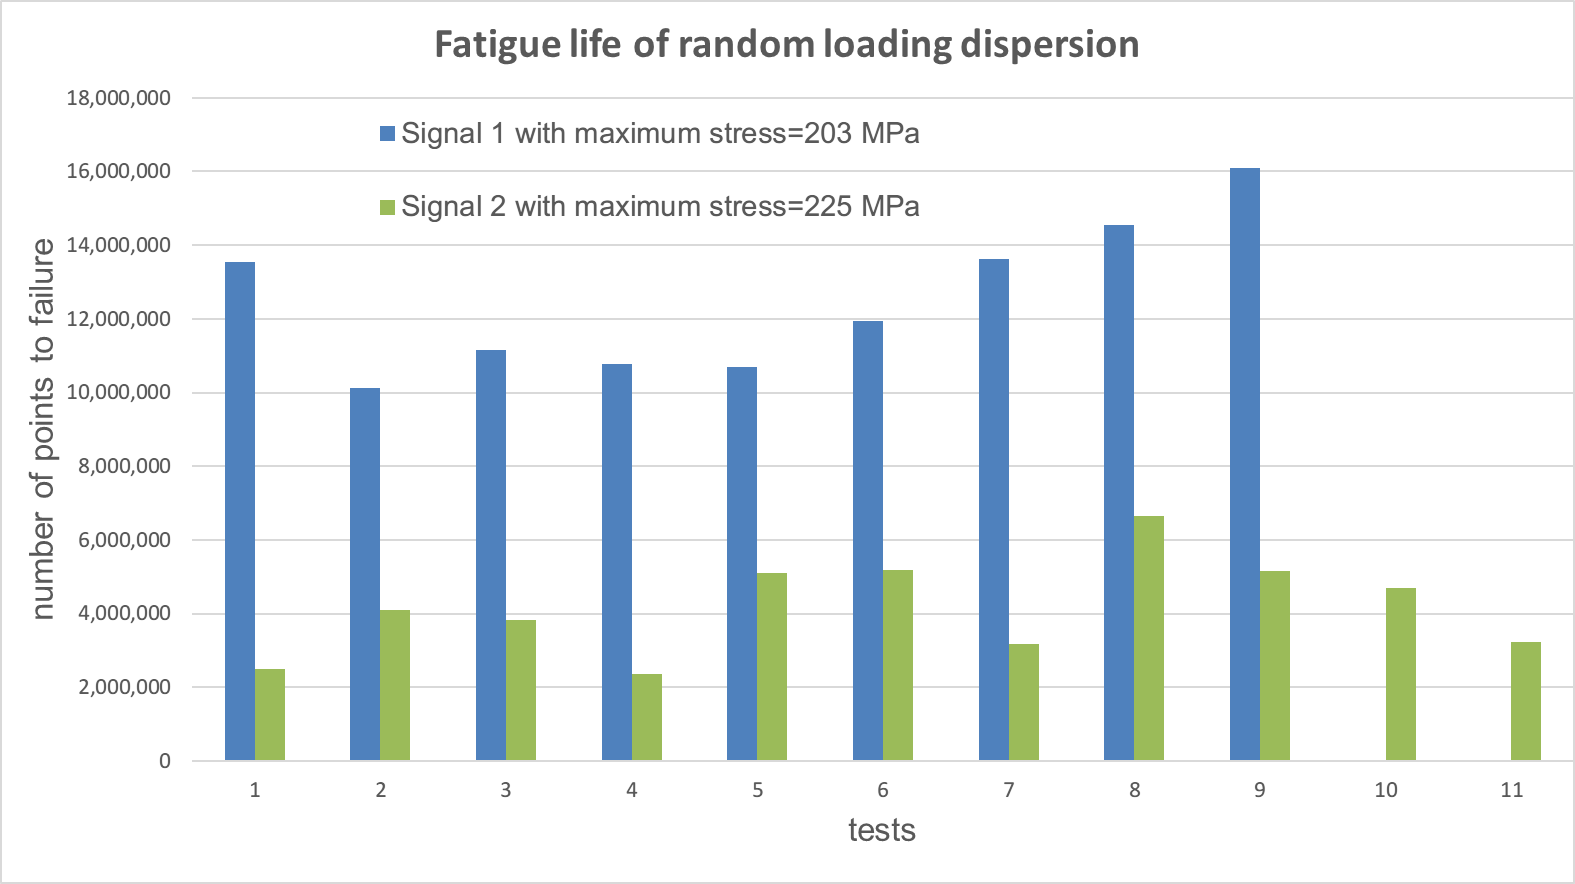
\includegraphics[width=\textwidth]{figures//randomdispersion.png} 
	\caption{Fatigue life of random loading dispersion}
	\label{fig.randomdispersion}
\end{figure}

After comparison with the experimental data we find out that large stresses cause much more damage than the smaller ones. It is necessary to include this major stress induced damage to our stress intensity parameter $\alpha$. With the new $\alpha$ used in Eq.\eqref{eq.final3} compared to Eq.\eqref{eq.alpha} we are able to calibrate our model better with the experimental results by using 
\begin{equation}
\alpha=1-a\left(  \dfrac{\frac{1}{s_{min}}}{1-\frac{1}{s_{min}}} \right) ^{f}.
\label{eq.majoralp}
\end{equation}


With $f=1.1$, we use the power to magnify large stress impact and minify lower stress damage.  The demonstration of major damage effect using magnification power is depicted in \figref{fig.sequenceours}. With larger value of power, the sequence effect is more significant(bigger dispersion between high-low and low-high sequence).

\begin{figure}[!h]
\centering
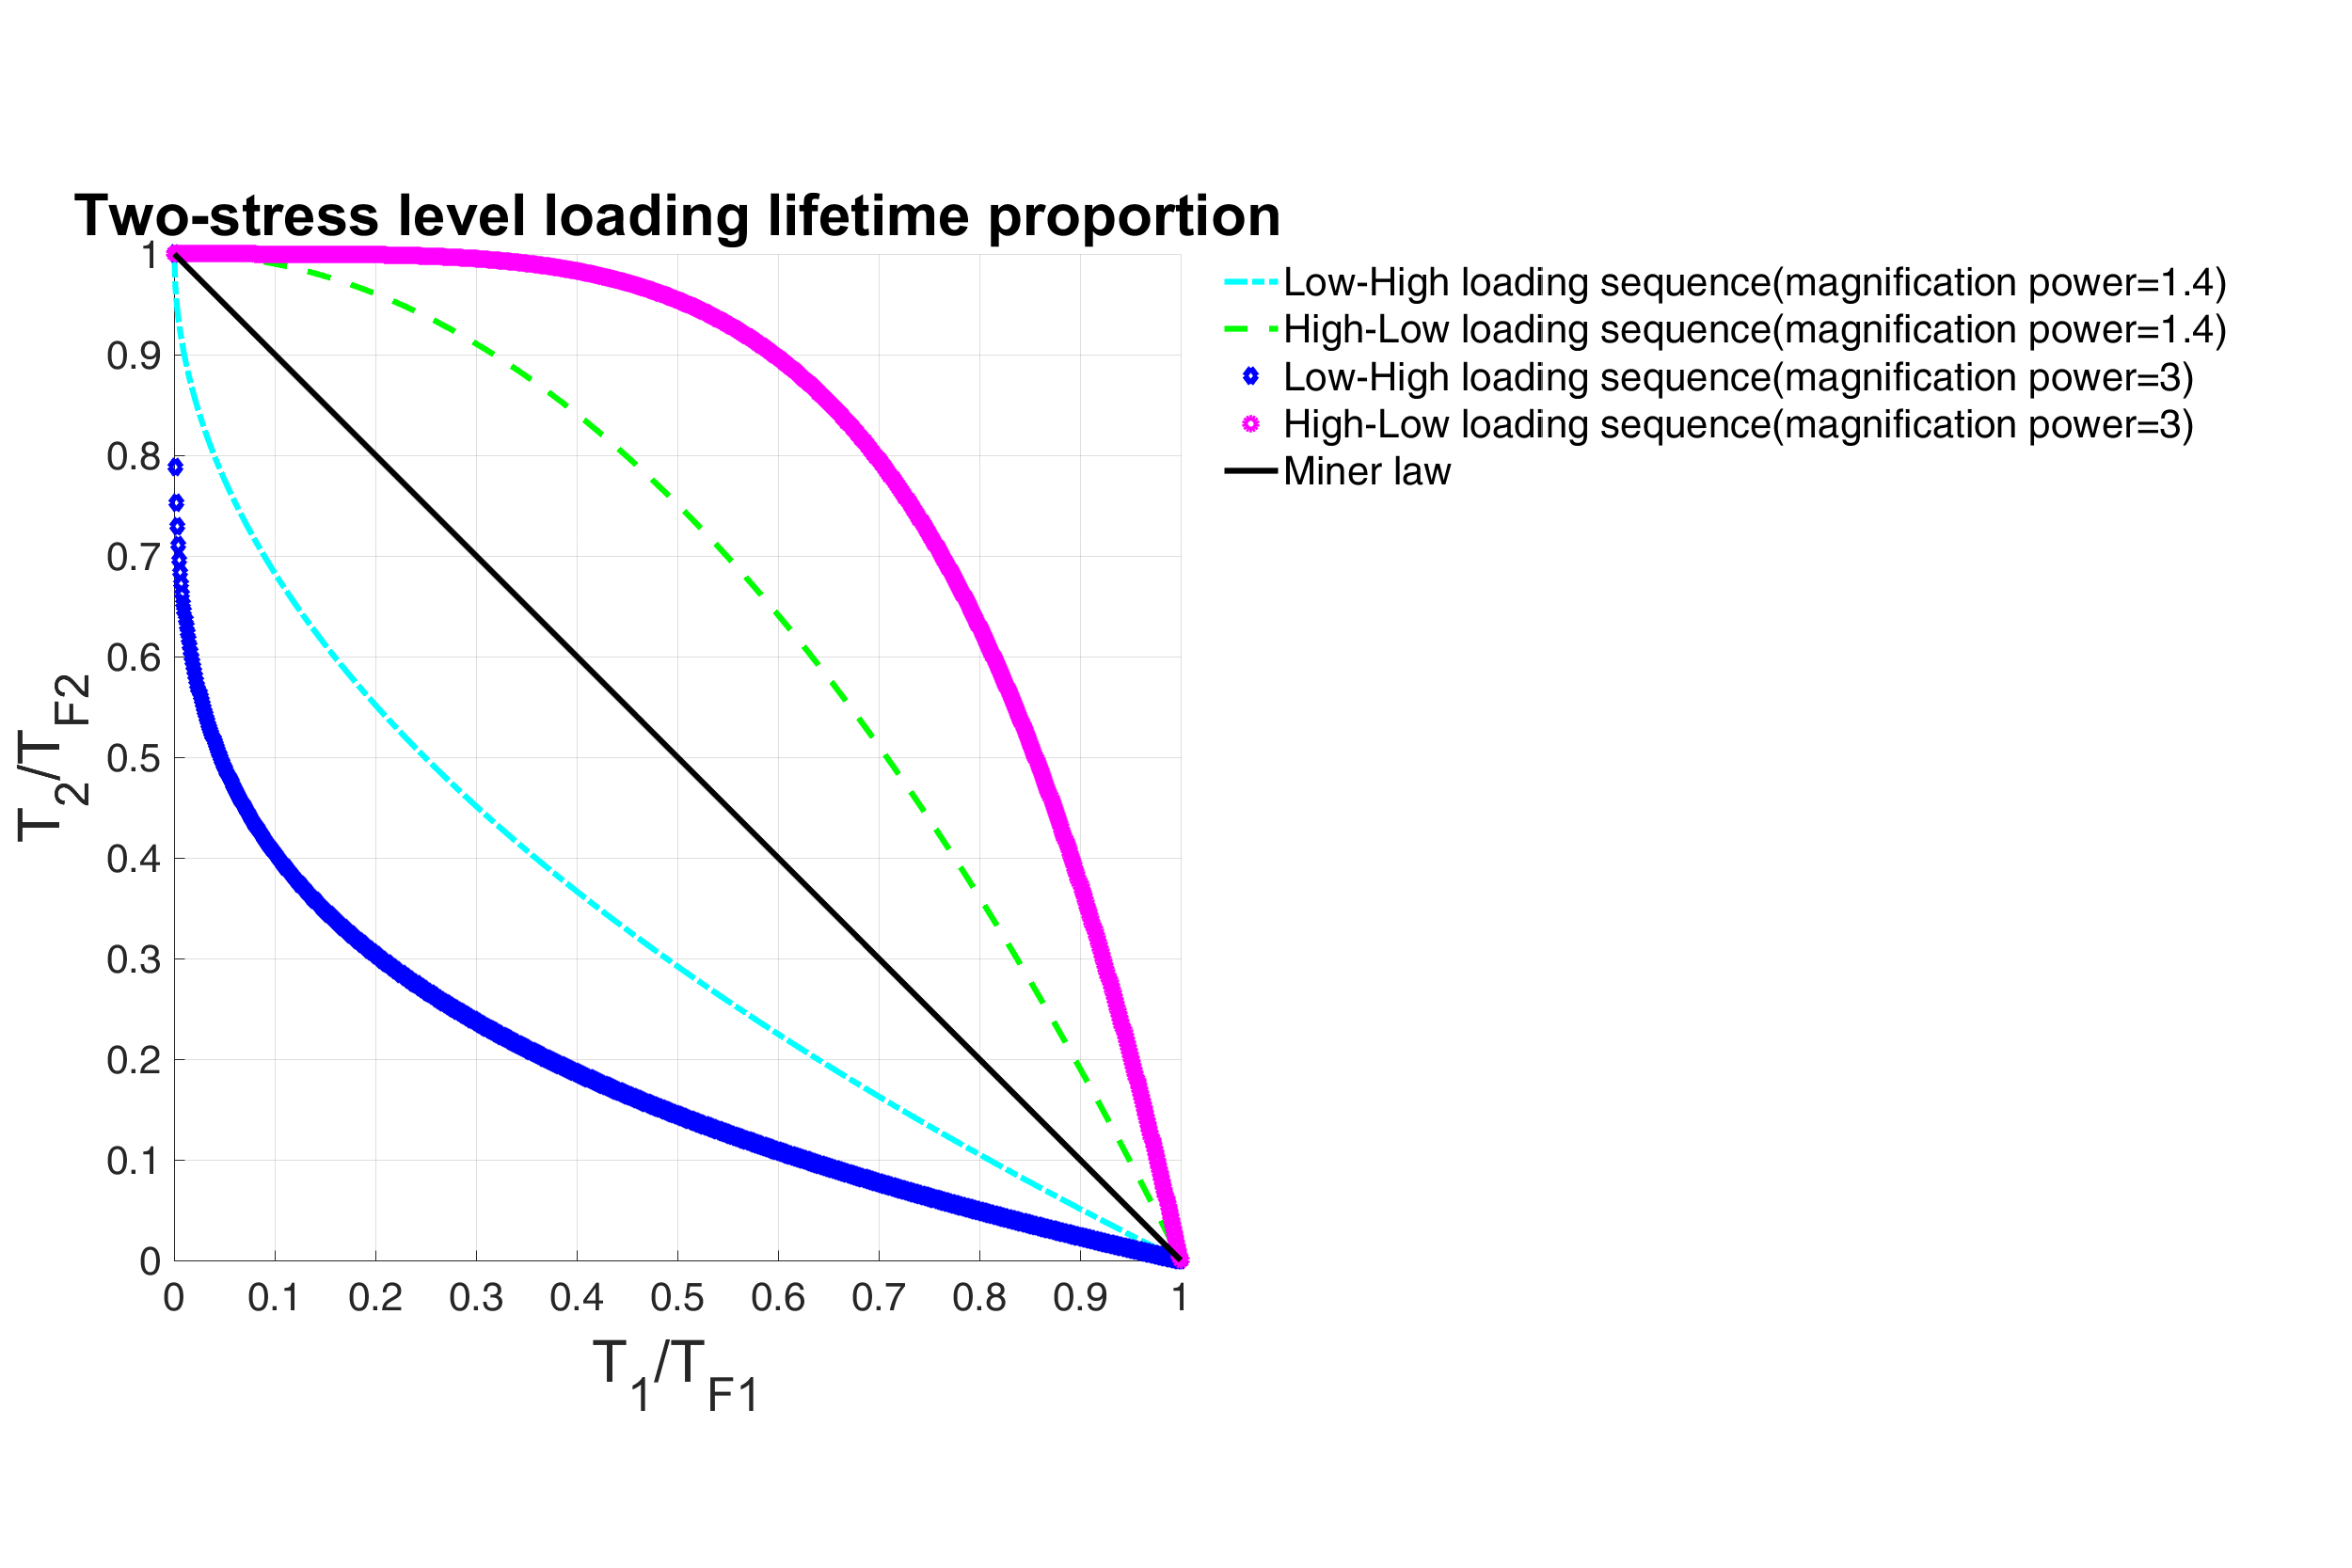
\includegraphics[width=\textwidth]{figures//sequence_ours.png} 
\caption{Major damage effect using different magnification power of Eq.\eqref{eq.majoralp} on sequence effect. Here high stress is 1MPa and low stress is 0.8MPa. We see that using a large power $f$ in Eq.\eqref{eq.majoralp} induces a stronger sequence effect.}
\label{fig.sequenceours}
\end{figure}

The larger value of $S_{a}$ causes more damage in the presence of the power $\beta$, leading to faster increase of 
$$(1-\alpha)=a\left(  \dfrac{\frac{1}{s_{min}}}{1-\frac{1}{s_{min}}} \right) ^{f}=a(s_{min}-1)^{-f}.$$ 
which causes faster damage accumulation. We can also see this effect in \figref{fig.SmaxSequence}. 

To assess large stress correctly we define the larger stress intensity as the value of stress which makes expression in the bracket in the second term of $\alpha$ greater than 1($ \dfrac{1}{ s_{min}(t)-1 }>1$), then we use power $\beta$ to magnify this term. In this way the damage is accelerated for large stresses. The deviatoric stress $S_{a}$, above which the damage is magnified,  is determined from: 
$$\alpha(t)=1-a\left( \dfrac{1}{ s_{min}(t)-1 } \right)^{1.1},$$
$$s_{min}(t)=\dfrac{\Sigma_y-\lambda \Sigma_H(t)}{S_{a}(t)}<2,$$
$$S_{large}(t)>\dfrac{\Sigma_y-\lambda \Sigma_H(t)}{2}.$$ 

The major damage effect can be seen in \figref{fig.SmaxSequence}, which occurs when $S$ is more than half the macroscopic yield stress of the material.

\begin{figure}[!h]
\centering
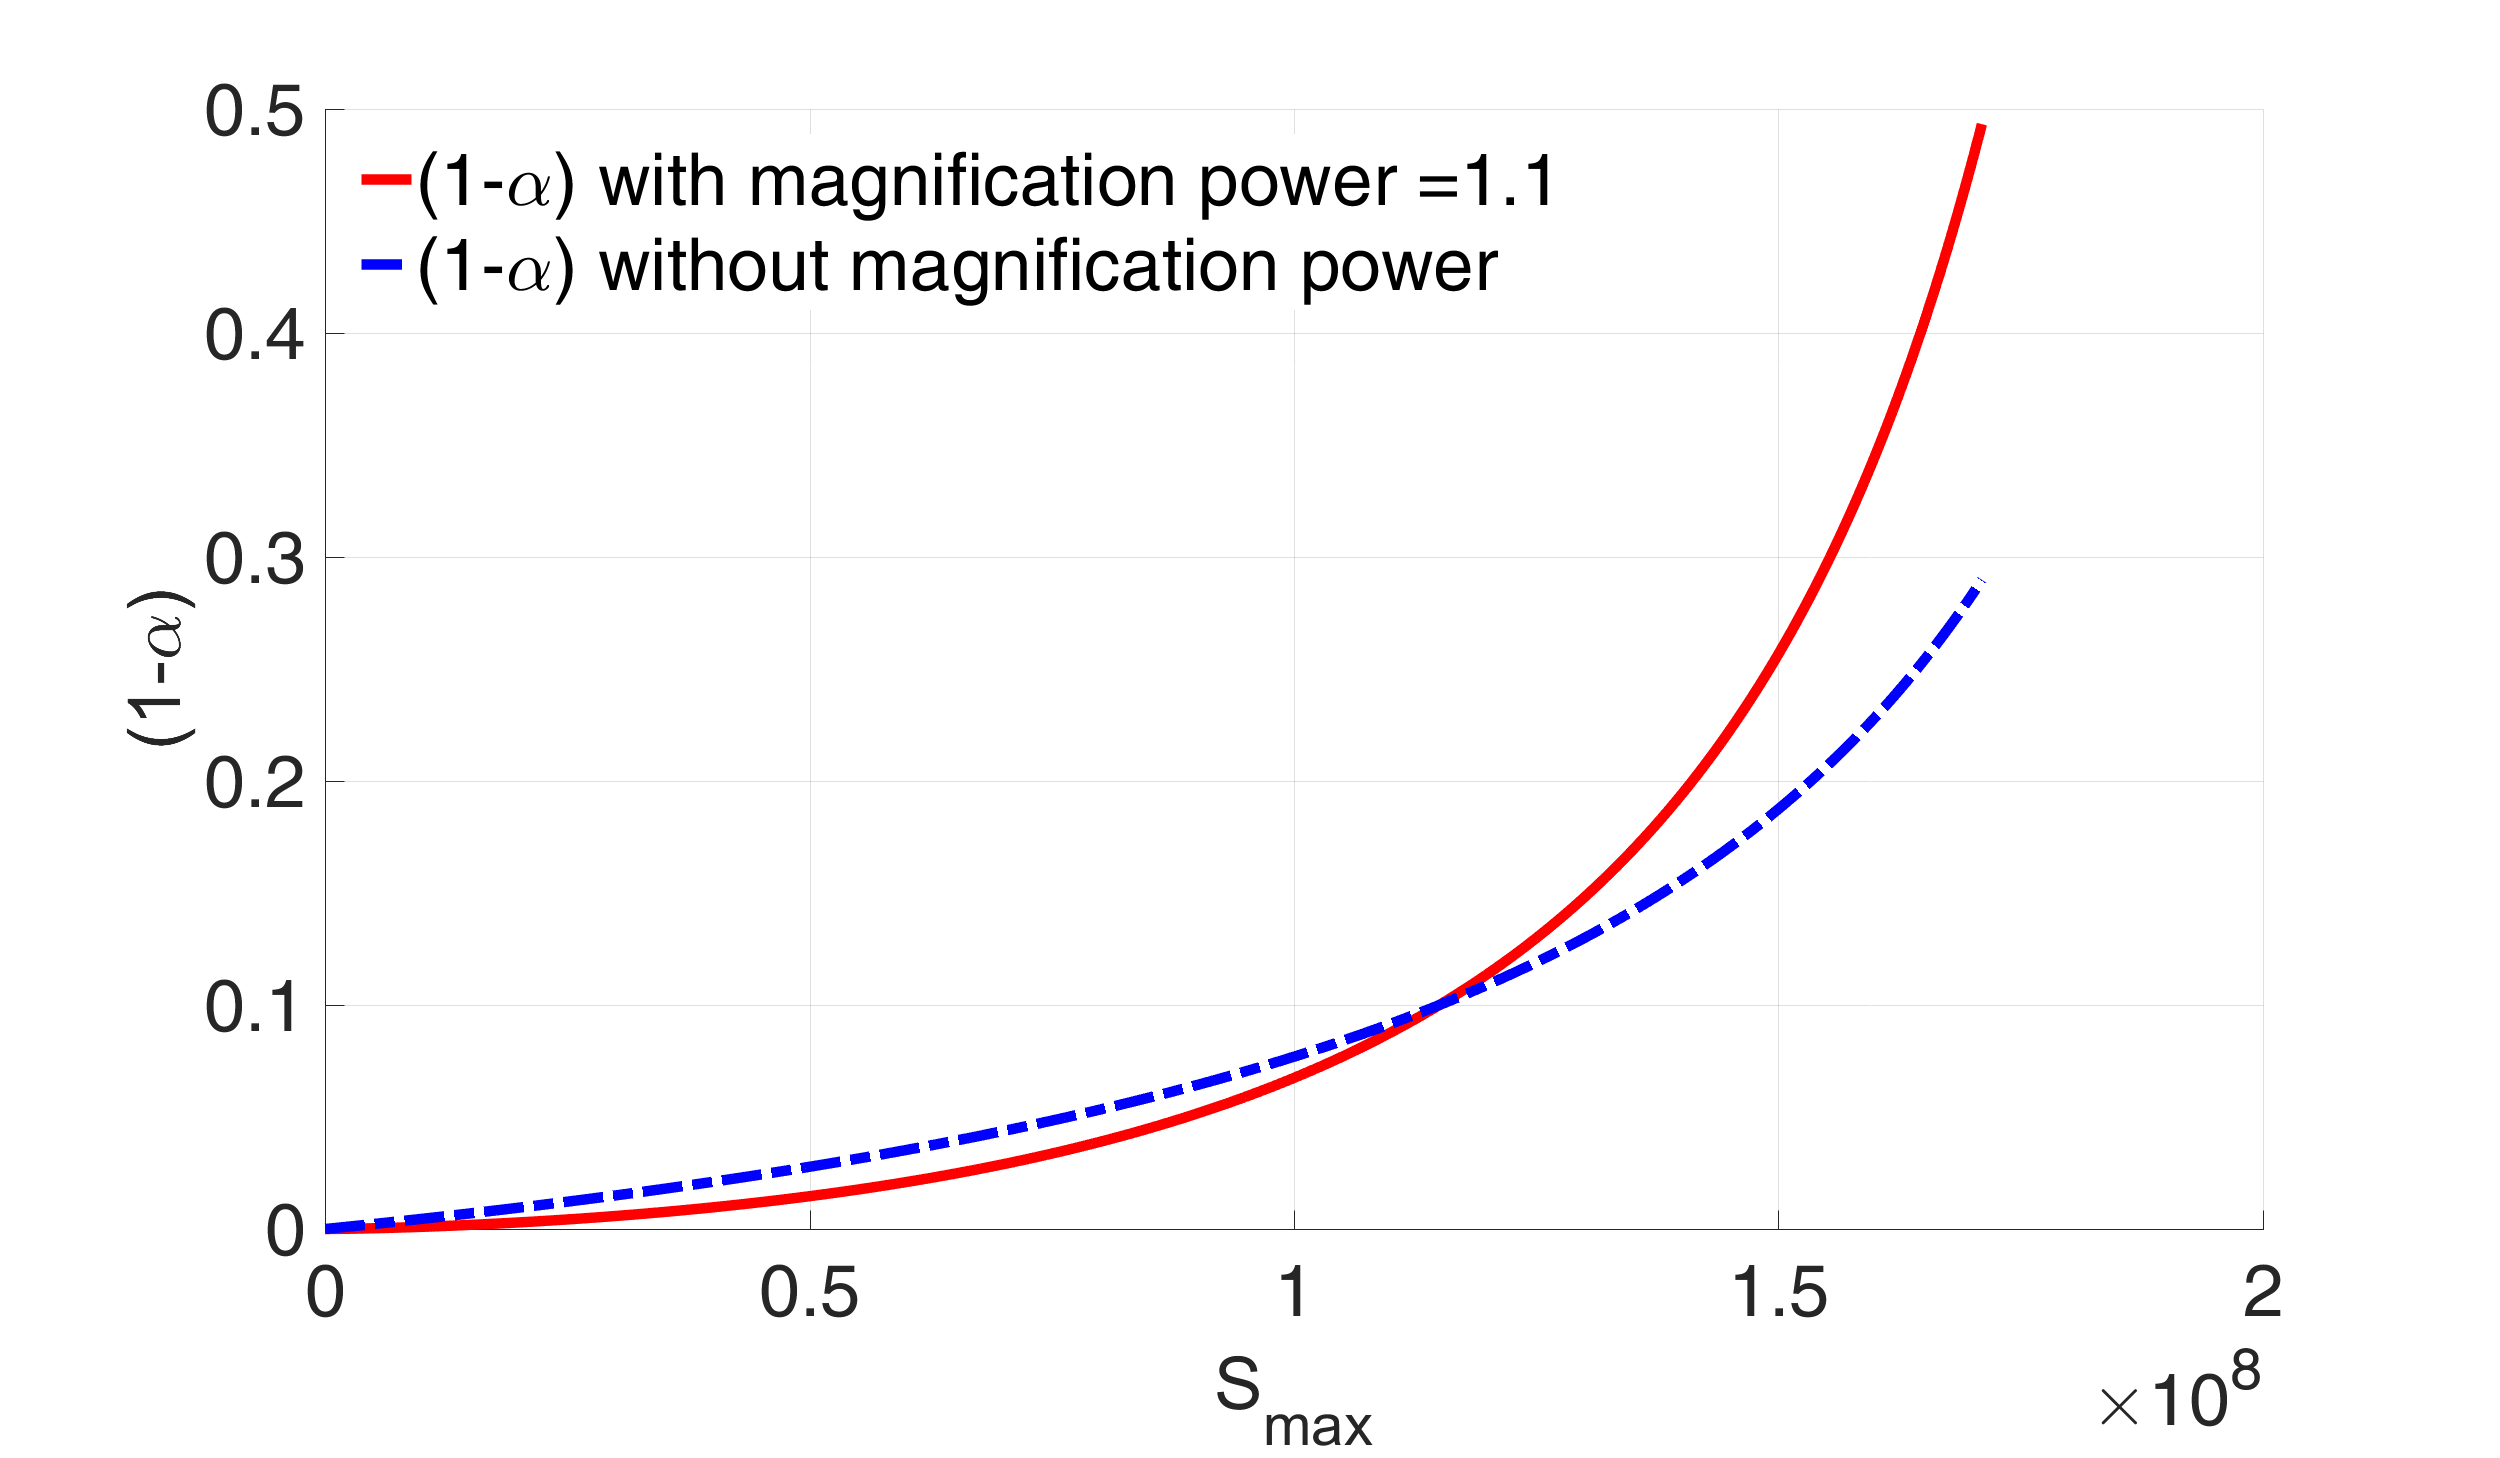
\includegraphics[width=\textwidth]{figures//alp_Smax_fb.png} 
\caption{(1-$\alpha$) term which stands for the load intensity evolution, both with and without the magnification power $f$}
\label{fig.SmaxSequence}
\end{figure}

\clearpage
\section{Identification strategy}
\label{sec:5.9}
In our tests we keep $f=1.1$(justified in Chapter \ref{chp:6} by \figref{fig.Cetimerralpfix} and \figref{fig.Cetimerr}). The positive hydrostatic stress and negative one have different effect on the yield limit. It is necessary to adopt 2 parameters to describe this behavior. So we divide the hydrostatic sensitivity $\lambda$ into 2 parts. $\lambda_+$ and $\lambda_-$. In the analytical formula, the amplitude of the stress intensity is adopted and the average value of tension hydrostatic stress(+) and compressive hydrostatic stress(-) is introduced.

For a good lifetime prediction, it is necessary to first identify the appropriate parameters of the model. For this purpose, we use the analytical formula Eq.\eqref{eq.cycNF} obtained in uniaxial cyclic loading case. With distinction of the hydrostatic stress in the presence of non-zero mean stress and since in fully reversed uniaxial loading we spend an equal time in compression and in traction, Eq.\eqref{eq:w} now writes:

\begin{equation}
W_{cyc}=\dfrac{2(E-k)(1+\nu)\left( \beta-1\right) }{ E(E+k\nu)\beta\left( \beta+1\right) }\left[ \dfrac{S_{a}^{\beta+1}}{ \left(\sigma_y-\lambda_+ \overline{\Sigma}_{H+}(t)\right)^{\beta-1}}+\dfrac{S_{a}^{\beta+1}}{ \left(\sigma_y-\lambda_- \overline{\Sigma}_{H-}(t)\right)^{\beta-1}}\right] .
\label{eq:wcycnew}
\end{equation}

\begin{equation}N_{Fnum}=\dfrac{W_0}{\left( 1-\alpha\right) }\dfrac{E(E+k\nu)\beta\left( \beta+1\right) }{ 2(E-k)(1+\nu)\left( \beta-1\right) }\dfrac{1}{\dfrac{S_{a}^{\beta+1}}{\left(\sigma_y-\lambda_+\overline{\Sigma}_{H+}(t)\right)^{\beta-1}}+\dfrac{S_{a}^{\beta+1}}{\left(\sigma_y-\lambda_-\overline{\Sigma}_{H-}(t)\right)^{\beta-1}}}.\label{eq:NFnew}
\end{equation}


To use our analytical model Eq.\eqref{eq:NFnew} to fit the experiments, we employ matlab Least-Squares (model fitting) algorithm. 

The best fitted parameters in uniaxial cyclic loading case are deduced from the minimization of the sum of square of difference between uniaxial numerical and experimental results:
\begin{equation}
\min_{\beta,\lambda,W_0}\left\lbrace \sum_{i}\left(N_{Fnum}-N_{Fexp} \right)^2\right\rbrace 
\label{eq.leastsquares}
\end{equation}

Assume there are $i$ sets of experimental data. To clarify the identification process, let us separate the parameters into:
\begin{itemize}
	\item Experimental data: $S_{a(i)}$, $\Sigma_{H(i)}$, $N_{Fexp(i)}$, $\sigma_y$, $E$, $k$, $\nu$.
	\item Material constants: $\beta$, $\lambda_{+-}$, $W_0$ (to be fitted)
	\item Input data from experimental data: $S_{max(i)}$, $\Sigma_{H(i)}$
	\item Input data from experimental data and parameter constants: $\alpha_{(i)}$
	\item Output data: $N_{Fnum(i)}$
\end{itemize}

In this process, $\sigma_y$, $E$, $k$ and $\nu$ are given elastoplastic material constants. For each test (i), the load parameters are maximum amplitude $S_{a(i)}$, mean hydrostatic stress $\overline{\Sigma}_{H(i)}$, and the experimental number of cycles to failure is given by $N_{Fexp(i)}$.

The exponent $\alpha_{(i)}$ is cycle average obtained by
\begin{equation}
\alpha_{(i)}=mean\left[1-a\left( \dfrac{1}{\dfrac{\Sigma_y-\lambda_{+-} \Sigma_{H}(t)}{S_{a}(t)}-1 } \right)^{1.1}\right] (i).
\label{eq.meanalp}
\end{equation}

The parameters to be calibrated are $W_0$, $\beta$ and $\lambda$. Since the exponent $\alpha_{(i)}$ depends on $\beta$ and $\lambda$, we proceed iteratively by:

\begin{enumerate}
	\item We first identify the S-N curve slope $\beta$ and the energy scale $W_0$ using the analytical formula with torsion tests because there is no $\lambda_{+-}$ impact in this kind of loading. We start from an initial guess $\beta$ from which we can deduce $\alpha_{(i)}$ by  numerical calculation of Eq.\ref{eq.meanalp} and identify $\beta$ and $W_0$ by least squares. Because our analytical formula is not derivable in all ranges, when the identified value of $\beta$ or $W_0$ get stuck in local minimum value, we regenerate a random $\beta$ or $W_0$ in their range so as to get the global least square value.
	\item Then, the parameter $\lambda_{+}$ are identified from numerical bending tests and we keep $\lambda_-=0$. The final parameters correspond to the $\lambda$ leading to the lowest identification error in $\beta$ and $W_0$. This strategy handles the nonlinearity in $\beta$ and is well adapted to the low sensitivity in $\lambda$.
\end{enumerate}



The analytical formula Eq.\eqref{eq:NFnew} with mean stress effect converges with the numerical method very well in the case of small $\beta$ and $\lambda_{+-}$. 


\textbf{Parameter sensitivity analysis}

The parameters we introduced during the deduction need to be calibrated. The source of the parameter identification are listed in Table.\ref{paras}.
We perform a sensitivity analysis to see the influence of each parameter by comparing the results obtained respectively for the reference value, an upper bound and a lower bound of each parameter.

\begin{table}[!h]
	\centering
	\begin{tabular}{l|c}
		\hline
		\textbf{Parameters}                                  & \multicolumn{1}{c}{\textbf{Strategy}} \\ \hline
		Hydrostatic pressure sensitivity $\lambda_+$           & hydrostatic stress sensitivity (identified)         \\
		Non-linearity of damage accumulation  $a$        & amplification factor of load intensity (guessed)     \\
		Weakening scales distribution exponent  $\beta$      & to be calibrated (identified)                   \\
		Dissipated energy to failure per defect  $W_0$ & energy scaling (identified)              \\ \hline
	\end{tabular}
	\caption{Parameters concerned}
	\label{paras}
\end{table}

We analyze the sensitivity of parameters separately as in Table.\ref{tab.sensitivity_const1}(uniaxial) and Table.\ref{tab.sensitivity_random1}(random loading). The parameter $\beta$ has more influence on the random loading case because it acts not only as the S-N curve slope but also the power magnification factor of large stress intensity. The $\lambda$ has little influence because both tests are conducted on very small or zero mean stress load history.


In Miner's law the parameter $\alpha$ is zero, the maximum value is below 1. For $\alpha=1$ the damage accumulation line becomes flat and there will be unlimited lifetime. To keep $\alpha$ in the range of $[0,1]$ where in random amplitude tests there is $S_{a}=163.3MPa$; we set the sensitivity of load intensity  $a$  to a maximum value of $0.29$ to keep $\alpha$ positive. 

The weakening scale distribution exponent(also the slope of S-N curve of the material) $\beta$ ranges from $1$ to $5$. The hydrostatic pressure sensitivity $\lambda$ is from positive mean stress test, which has the range of $0\sim0.8$. In constant amplitude cyclic loading, the dissipated energy to failure per defect $W_0$(in MPa) is related to fatigue lifetime of the material.

\begin{table}[!h]
	\centering
	\begin{tabular}{lrrrrrrr}
		\hline
		\multicolumn{8}{c}{\textbf{Constant amplitude sensitivity test with $f(\beta)=\beta$}}                                                                                                                                                                                                                                           \\ \hline
		& \multicolumn{1}{r}{\textbf{Ref}} & \multicolumn{1}{r}{\textbf{Min}} & \multicolumn{1}{r}{\textbf{Max}} & \multicolumn{1}{r}{\textbf{Ref\_n}} & \multicolumn{1}{r}{\textbf{Min\_n}} & \multicolumn{1}{r}{\textbf{Max\_n}} & \multicolumn{1}{r}{\textbf{Sensitivity}} \\ \hline
		\textbf{$\beta$}   & 1.1                                          & 1.05                             & 1.50                             & 414233                                     & 
		783723 	                              & 243300 
		&-3.19 
		\\
		\textbf{$\lambda_+$} & 0.1                                          & 0.05                             & 0.50                             & 414233                                    & 449598 
		& 443376 
		& 0.00                                    \\
		\textbf{$W_0$}     & 3.27e8                                     & 1.00e8                         & 5.00e8                         & 414233                                     & 137498 
		& 687209 
		& 1.08                                    \\
		\textbf{$a$}       & 0.1                                          & 0.05                             & 0.15                             & 414233                                  & 672869 
		& 324754 
		& -0.84                                   \\ \hline
	\end{tabular}
	\caption{Example of parameters sensitivity at cyclic loading of BATCH\_A\_02 on AW-6106 T6 aluminum (table.\ref{tab:Cetim})}
	\label{tab.sensitivity_const1}
\end{table}

\clearpage
